\documentclass[twoside]{book}

% Packages required by doxygen
\usepackage{fixltx2e}
\usepackage{calc}
\usepackage{doxygen}
\usepackage[export]{adjustbox} % also loads graphicx
\usepackage{graphicx}
\usepackage[utf8]{inputenc}
\usepackage{makeidx}
\usepackage{multicol}
\usepackage{multirow}
\PassOptionsToPackage{warn}{textcomp}
\usepackage{textcomp}
\usepackage[nointegrals]{wasysym}
\usepackage[table]{xcolor}

% Font selection
\usepackage[T1]{fontenc}
\usepackage[scaled=.90]{helvet}
\usepackage{courier}
\usepackage{amssymb}
\usepackage{sectsty}
\renewcommand{\familydefault}{\sfdefault}
\allsectionsfont{%
  \fontseries{bc}\selectfont%
  \color{darkgray}%
}
\renewcommand{\DoxyLabelFont}{%
  \fontseries{bc}\selectfont%
  \color{darkgray}%
}
\newcommand{\+}{\discretionary{\mbox{\scriptsize$\hookleftarrow$}}{}{}}

% Page & text layout
\usepackage{geometry}
\geometry{%
  a4paper,%
  top=2.5cm,%
  bottom=2.5cm,%
  left=2.5cm,%
  right=2.5cm%
}
\tolerance=750
\hfuzz=15pt
\hbadness=750
\setlength{\emergencystretch}{15pt}
\setlength{\parindent}{0cm}
\setlength{\parskip}{3ex plus 2ex minus 2ex}
\makeatletter
\renewcommand{\paragraph}{%
  \@startsection{paragraph}{4}{0ex}{-1.0ex}{1.0ex}{%
    \normalfont\normalsize\bfseries\SS@parafont%
  }%
}
\renewcommand{\subparagraph}{%
  \@startsection{subparagraph}{5}{0ex}{-1.0ex}{1.0ex}{%
    \normalfont\normalsize\bfseries\SS@subparafont%
  }%
}
\makeatother

% Headers & footers
\usepackage{fancyhdr}
\pagestyle{fancyplain}
\fancyhead[LE]{\fancyplain{}{\bfseries\thepage}}
\fancyhead[CE]{\fancyplain{}{}}
\fancyhead[RE]{\fancyplain{}{\bfseries\leftmark}}
\fancyhead[LO]{\fancyplain{}{\bfseries\rightmark}}
\fancyhead[CO]{\fancyplain{}{}}
\fancyhead[RO]{\fancyplain{}{\bfseries\thepage}}
\fancyfoot[LE]{\fancyplain{}{}}
\fancyfoot[CE]{\fancyplain{}{}}
\fancyfoot[RE]{\fancyplain{}{\bfseries\scriptsize Generated by Doxygen }}
\fancyfoot[LO]{\fancyplain{}{\bfseries\scriptsize Generated by Doxygen }}
\fancyfoot[CO]{\fancyplain{}{}}
\fancyfoot[RO]{\fancyplain{}{}}
\renewcommand{\footrulewidth}{0.4pt}
\renewcommand{\chaptermark}[1]{%
  \markboth{#1}{}%
}
\renewcommand{\sectionmark}[1]{%
  \markright{\thesection\ #1}%
}

% Indices & bibliography
\usepackage{natbib}
\usepackage[titles]{tocloft}
\setcounter{tocdepth}{3}
\setcounter{secnumdepth}{5}
\makeindex

% Hyperlinks (required, but should be loaded last)
\usepackage{ifpdf}
\ifpdf
  \usepackage[pdftex,pagebackref=true]{hyperref}
\else
  \usepackage[ps2pdf,pagebackref=true]{hyperref}
\fi
\hypersetup{%
  colorlinks=true,%
  linkcolor=blue,%
  citecolor=blue,%
  unicode%
}

% Custom commands
\newcommand{\clearemptydoublepage}{%
  \newpage{\pagestyle{empty}\cleardoublepage}%
}

\usepackage{caption}
\captionsetup{labelsep=space,justification=centering,font={bf},singlelinecheck=off,skip=4pt,position=top}

%===== C O N T E N T S =====

\begin{document}

% Titlepage & ToC
\hypersetup{pageanchor=false,
             bookmarksnumbered=true,
             pdfencoding=unicode
            }
\pagenumbering{alph}
\begin{titlepage}
\vspace*{7cm}
\begin{center}%
{\Large Cipher Analyser \\[1ex]\large 0.\+1 }\\
\vspace*{1cm}
{\large Generated by Doxygen 1.8.13}\\
\end{center}
\end{titlepage}
\clearemptydoublepage
\pagenumbering{roman}
\tableofcontents
\clearemptydoublepage
\pagenumbering{arabic}
\hypersetup{pageanchor=true}

%--- Begin generated contents ---
\chapter{Namespace Index}
\section{Namespace List}
Here is a list of all documented namespaces with brief descriptions\+:\begin{DoxyCompactList}
\item\contentsline{section}{\hyperlink{namespaceoption}{option} \\*The namespace of The Lean Mean C++ \hyperlink{classoption_1_1Option}{Option} \hyperlink{classoption_1_1Parser}{Parser} }{\pageref{namespaceoption}}{}
\end{DoxyCompactList}

\chapter{Hierarchical Index}
\section{Class Hierarchy}
This inheritance list is sorted roughly, but not completely, alphabetically\+:\begin{DoxyCompactList}
\item \contentsline{section}{option\+:\+:Parser\+:\+:Action}{\pageref{structoption_1_1Parser_1_1Action}}{}
\begin{DoxyCompactList}
\item \contentsline{section}{option\+:\+:Parser\+:\+:Store\+Option\+Action}{\pageref{classoption_1_1Parser_1_1StoreOptionAction}}{}
\item \contentsline{section}{option\+:\+:Stats\+:\+:Count\+Options\+Action}{\pageref{classoption_1_1Stats_1_1CountOptionsAction}}{}
\end{DoxyCompactList}
\item \contentsline{section}{option\+:\+:Arg}{\pageref{structoption_1_1Arg}}{}
\begin{DoxyCompactList}
\item \contentsline{section}{Arg}{\pageref{structArg}}{}
\end{DoxyCompactList}
\item \contentsline{section}{option\+:\+:Descriptor}{\pageref{structoption_1_1Descriptor}}{}
\item \contentsline{section}{File\+Manager}{\pageref{classFileManager}}{}
\item \contentsline{section}{Frequency}{\pageref{classFrequency}}{}
\item \contentsline{section}{Friedmann}{\pageref{classFriedmann}}{}
\item \contentsline{section}{option\+:\+:Print\+Usage\+Implementation\+:\+:I\+String\+Writer}{\pageref{structoption_1_1PrintUsageImplementation_1_1IStringWriter}}{}
\begin{DoxyCompactList}
\item \contentsline{section}{option\+:\+:Print\+Usage\+Implementation\+:\+:Function\+Writer$<$ Function $>$}{\pageref{structoption_1_1PrintUsageImplementation_1_1FunctionWriter}}{}
\item \contentsline{section}{option\+:\+:Print\+Usage\+Implementation\+:\+:O\+Stream\+Writer$<$ O\+Stream $>$}{\pageref{structoption_1_1PrintUsageImplementation_1_1OStreamWriter}}{}
\item \contentsline{section}{option\+:\+:Print\+Usage\+Implementation\+:\+:Stream\+Writer$<$ Function, Stream $>$}{\pageref{structoption_1_1PrintUsageImplementation_1_1StreamWriter}}{}
\item \contentsline{section}{option\+:\+:Print\+Usage\+Implementation\+:\+:Syscall\+Writer$<$ Syscall $>$}{\pageref{structoption_1_1PrintUsageImplementation_1_1SyscallWriter}}{}
\item \contentsline{section}{option\+:\+:Print\+Usage\+Implementation\+:\+:Temporary\+Writer$<$ Temporary $>$}{\pageref{structoption_1_1PrintUsageImplementation_1_1TemporaryWriter}}{}
\end{DoxyCompactList}
\item \contentsline{section}{Kasiski}{\pageref{classKasiski}}{}
\item \contentsline{section}{Kerckhoff}{\pageref{classKerckhoff}}{}
\item \contentsline{section}{Key\+Brute}{\pageref{classKeyBrute}}{}
\item \contentsline{section}{Key\+Eliminator}{\pageref{classKeyEliminator}}{}
\item \contentsline{section}{Language}{\pageref{classLanguage}}{}
\begin{DoxyCompactList}
\item \contentsline{section}{English}{\pageref{classEnglish}}{}
\end{DoxyCompactList}
\item \contentsline{section}{option\+:\+:Print\+Usage\+Implementation\+:\+:Line\+Part\+Iterator}{\pageref{classoption_1_1PrintUsageImplementation_1_1LinePartIterator}}{}
\item \contentsline{section}{option\+:\+:Print\+Usage\+Implementation\+:\+:Line\+Wrapper}{\pageref{classoption_1_1PrintUsageImplementation_1_1LineWrapper}}{}
\item \contentsline{section}{option\+:\+:Option}{\pageref{classoption_1_1Option}}{}
\item \contentsline{section}{option\+:\+:Parser}{\pageref{classoption_1_1Parser}}{}
\item \contentsline{section}{option\+:\+:Print\+Usage\+Implementation}{\pageref{structoption_1_1PrintUsageImplementation}}{}
\item \contentsline{section}{Rel\+Frequency}{\pageref{classRelFrequency}}{}
\item \contentsline{section}{option\+:\+:Stats}{\pageref{structoption_1_1Stats}}{}
\item \contentsline{section}{Vigenere}{\pageref{classVigenere}}{}
\end{DoxyCompactList}

\chapter{Class Index}
\section{Class List}
Here are the classes, structs, unions and interfaces with brief descriptions\+:\begin{DoxyCompactList}
\item\contentsline{section}{\hyperlink{structoption_1_1Parser_1_1Action}{option\+::\+Parser\+::\+Action} }{\pageref{structoption_1_1Parser_1_1Action}}{}
\item\contentsline{section}{\hyperlink{structArg}{Arg} }{\pageref{structArg}}{}
\item\contentsline{section}{\hyperlink{structoption_1_1Arg}{option\+::\+Arg} \\*Functions for checking the validity of option arguments }{\pageref{structoption_1_1Arg}}{}
\item\contentsline{section}{\hyperlink{classoption_1_1Stats_1_1CountOptionsAction}{option\+::\+Stats\+::\+Count\+Options\+Action} }{\pageref{classoption_1_1Stats_1_1CountOptionsAction}}{}
\item\contentsline{section}{\hyperlink{structoption_1_1Descriptor}{option\+::\+Descriptor} \\*Describes an option, its help text (usage) and how it should be parsed }{\pageref{structoption_1_1Descriptor}}{}
\item\contentsline{section}{\hyperlink{classEnglish}{English} }{\pageref{classEnglish}}{}
\item\contentsline{section}{\hyperlink{classFileManager}{File\+Manager} }{\pageref{classFileManager}}{}
\item\contentsline{section}{\hyperlink{classFrequency}{Frequency} }{\pageref{classFrequency}}{}
\item\contentsline{section}{\hyperlink{classFriedmann}{Friedmann} }{\pageref{classFriedmann}}{}
\item\contentsline{section}{\hyperlink{structoption_1_1PrintUsageImplementation_1_1FunctionWriter}{option\+::\+Print\+Usage\+Implementation\+::\+Function\+Writer$<$ Function $>$} }{\pageref{structoption_1_1PrintUsageImplementation_1_1FunctionWriter}}{}
\item\contentsline{section}{\hyperlink{structoption_1_1PrintUsageImplementation_1_1IStringWriter}{option\+::\+Print\+Usage\+Implementation\+::\+I\+String\+Writer} }{\pageref{structoption_1_1PrintUsageImplementation_1_1IStringWriter}}{}
\item\contentsline{section}{\hyperlink{classKasiski}{Kasiski} }{\pageref{classKasiski}}{}
\item\contentsline{section}{\hyperlink{classKerckhoff}{Kerckhoff} }{\pageref{classKerckhoff}}{}
\item\contentsline{section}{\hyperlink{classKeyBrute}{Key\+Brute} }{\pageref{classKeyBrute}}{}
\item\contentsline{section}{\hyperlink{classKeyEliminator}{Key\+Eliminator} }{\pageref{classKeyEliminator}}{}
\item\contentsline{section}{\hyperlink{classLanguage}{Language} }{\pageref{classLanguage}}{}
\item\contentsline{section}{\hyperlink{classoption_1_1PrintUsageImplementation_1_1LinePartIterator}{option\+::\+Print\+Usage\+Implementation\+::\+Line\+Part\+Iterator} }{\pageref{classoption_1_1PrintUsageImplementation_1_1LinePartIterator}}{}
\item\contentsline{section}{\hyperlink{classoption_1_1PrintUsageImplementation_1_1LineWrapper}{option\+::\+Print\+Usage\+Implementation\+::\+Line\+Wrapper} }{\pageref{classoption_1_1PrintUsageImplementation_1_1LineWrapper}}{}
\item\contentsline{section}{\hyperlink{classoption_1_1Option}{option\+::\+Option} \\*A parsed option from the command line together with its argument if it has one }{\pageref{classoption_1_1Option}}{}
\item\contentsline{section}{\hyperlink{structoption_1_1PrintUsageImplementation_1_1OStreamWriter}{option\+::\+Print\+Usage\+Implementation\+::\+O\+Stream\+Writer$<$ O\+Stream $>$} }{\pageref{structoption_1_1PrintUsageImplementation_1_1OStreamWriter}}{}
\item\contentsline{section}{\hyperlink{classoption_1_1Parser}{option\+::\+Parser} \\*Checks argument vectors for validity and parses them into data structures that are easier to work with }{\pageref{classoption_1_1Parser}}{}
\item\contentsline{section}{\hyperlink{structoption_1_1PrintUsageImplementation}{option\+::\+Print\+Usage\+Implementation} }{\pageref{structoption_1_1PrintUsageImplementation}}{}
\item\contentsline{section}{\hyperlink{classRelFrequency}{Rel\+Frequency} }{\pageref{classRelFrequency}}{}
\item\contentsline{section}{\hyperlink{structoption_1_1Stats}{option\+::\+Stats} \\*Determines the minimum lengths of the buffer and options arrays used for \hyperlink{classoption_1_1Parser}{Parser} }{\pageref{structoption_1_1Stats}}{}
\item\contentsline{section}{\hyperlink{classoption_1_1Parser_1_1StoreOptionAction}{option\+::\+Parser\+::\+Store\+Option\+Action} }{\pageref{classoption_1_1Parser_1_1StoreOptionAction}}{}
\item\contentsline{section}{\hyperlink{structoption_1_1PrintUsageImplementation_1_1StreamWriter}{option\+::\+Print\+Usage\+Implementation\+::\+Stream\+Writer$<$ Function, Stream $>$} }{\pageref{structoption_1_1PrintUsageImplementation_1_1StreamWriter}}{}
\item\contentsline{section}{\hyperlink{structoption_1_1PrintUsageImplementation_1_1SyscallWriter}{option\+::\+Print\+Usage\+Implementation\+::\+Syscall\+Writer$<$ Syscall $>$} }{\pageref{structoption_1_1PrintUsageImplementation_1_1SyscallWriter}}{}
\item\contentsline{section}{\hyperlink{structoption_1_1PrintUsageImplementation_1_1TemporaryWriter}{option\+::\+Print\+Usage\+Implementation\+::\+Temporary\+Writer$<$ Temporary $>$} }{\pageref{structoption_1_1PrintUsageImplementation_1_1TemporaryWriter}}{}
\item\contentsline{section}{\hyperlink{classVigenere}{Vigenere} }{\pageref{classVigenere}}{}
\end{DoxyCompactList}

\chapter{File Index}
\section{File List}
Here is a list of all documented files with brief descriptions\+:\begin{DoxyCompactList}
\item\contentsline{section}{headers/\hyperlink{FileManager_8hpp}{File\+Manager.\+hpp} }{\pageref{FileManager_8hpp}}{}
\item\contentsline{section}{headers/\hyperlink{Frequency_8hpp}{Frequency.\+hpp} }{\pageref{Frequency_8hpp}}{}
\item\contentsline{section}{headers/\hyperlink{KeyAnalyser_8hpp}{Key\+Analyser.\+hpp} }{\pageref{KeyAnalyser_8hpp}}{}
\item\contentsline{section}{headers/{\bfseries Key\+Brute.\+hpp} }{\pageref{KeyBrute_8hpp}}{}
\item\contentsline{section}{headers/\hyperlink{Language_8hpp}{Language.\+hpp} }{\pageref{Language_8hpp}}{}
\item\contentsline{section}{headers/\hyperlink{optionparser_8hpp}{optionparser.\+hpp} \\*This is the only file required to use The Lean Mean C++ Option Parser. Just \#include it and you\textquotesingle{}re set }{\pageref{optionparser_8hpp}}{}
\item\contentsline{section}{headers/\hyperlink{PolyCrack_8hpp}{Poly\+Crack.\+hpp} }{\pageref{PolyCrack_8hpp}}{}
\item\contentsline{section}{headers/\hyperlink{Vigenere_8hpp}{Vigenere.\+hpp} }{\pageref{Vigenere_8hpp}}{}
\item\contentsline{section}{sources/\hyperlink{Frequency_8cpp}{Frequency.\+cpp} }{\pageref{Frequency_8cpp}}{}
\item\contentsline{section}{sources/\hyperlink{KeyAnalyser_8cpp}{Key\+Analyser.\+cpp} }{\pageref{KeyAnalyser_8cpp}}{}
\item\contentsline{section}{sources/\hyperlink{main_8cpp}{main.\+cpp} }{\pageref{main_8cpp}}{}
\item\contentsline{section}{sources/\hyperlink{TextUtils_8cpp}{Text\+Utils.\+cpp} }{\pageref{TextUtils_8cpp}}{}
\item\contentsline{section}{sources/\hyperlink{Vigenere_8cpp}{Vigenere.\+cpp} }{\pageref{Vigenere_8cpp}}{}
\end{DoxyCompactList}

\chapter{Namespace Documentation}
\hypertarget{namespaceoption}{}\section{option Namespace Reference}
\label{namespaceoption}\index{option@{option}}


The namespace of The Lean Mean C++ \hyperlink{classoption_1_1Option}{Option} \hyperlink{classoption_1_1Parser}{Parser}.  


\subsection*{Classes}
\begin{DoxyCompactItemize}
\item 
struct \hyperlink{structoption_1_1Arg}{Arg}
\begin{DoxyCompactList}\small\item\em Functions for checking the validity of option arguments. \end{DoxyCompactList}\item 
struct \hyperlink{structoption_1_1Descriptor}{Descriptor}
\begin{DoxyCompactList}\small\item\em Describes an option, its help text (usage) and how it should be parsed. \end{DoxyCompactList}\item 
class \hyperlink{classoption_1_1Option}{Option}
\begin{DoxyCompactList}\small\item\em A parsed option from the command line together with its argument if it has one. \end{DoxyCompactList}\item 
class \hyperlink{classoption_1_1Parser}{Parser}
\begin{DoxyCompactList}\small\item\em Checks argument vectors for validity and parses them into data structures that are easier to work with. \end{DoxyCompactList}\item 
struct \hyperlink{structoption_1_1PrintUsageImplementation}{Print\+Usage\+Implementation}
\item 
struct \hyperlink{structoption_1_1Stats}{Stats}
\begin{DoxyCompactList}\small\item\em Determines the minimum lengths of the buffer and options arrays used for \hyperlink{classoption_1_1Parser}{Parser}. \end{DoxyCompactList}\end{DoxyCompactItemize}
\subsection*{Typedefs}
\begin{DoxyCompactItemize}
\item 
typedef \hyperlink{namespaceoption_aee8c76a07877335762631491e7a5a1a9}{Arg\+Status}($\ast$ \hyperlink{namespaceoption_a4cdf403efae65e18bf850e2001b12a2a}{Check\+Arg}) (const \hyperlink{classoption_1_1Option}{Option} \&option, bool msg)
\begin{DoxyCompactList}\small\item\em Signature of functions that check if an argument is valid for a certain type of option. \end{DoxyCompactList}\end{DoxyCompactItemize}
\subsection*{Enumerations}
\begin{DoxyCompactItemize}
\item 
enum \hyperlink{namespaceoption_aee8c76a07877335762631491e7a5a1a9}{Arg\+Status} \{ \hyperlink{namespaceoption_aee8c76a07877335762631491e7a5a1a9a353903b042e8eb0aa2f60c0043a58a7e}{A\+R\+G\+\_\+\+N\+O\+NE}, 
\hyperlink{namespaceoption_aee8c76a07877335762631491e7a5a1a9a445e08cb1747e5a22929e7ef2da43b55}{A\+R\+G\+\_\+\+OK}, 
\hyperlink{namespaceoption_aee8c76a07877335762631491e7a5a1a9a83e0837c79c957525918111d33cab3a9}{A\+R\+G\+\_\+\+I\+G\+N\+O\+RE}, 
\hyperlink{namespaceoption_aee8c76a07877335762631491e7a5a1a9a9528e32563b795bd2930b12d0a5e382d}{A\+R\+G\+\_\+\+I\+L\+L\+E\+G\+AL}
 \}\begin{DoxyCompactList}\small\item\em Possible results when checking if an argument is valid for a certain option. \end{DoxyCompactList}
\end{DoxyCompactItemize}
\subsection*{Functions}
\begin{DoxyCompactItemize}
\item 
{\footnotesize template$<$typename O\+Stream $>$ }\\void \hyperlink{namespaceoption_afc8bb7e040a98a0b33ff1ce9da1be0d1}{print\+Usage} (O\+Stream \&prn, const \hyperlink{structoption_1_1Descriptor}{Descriptor} usage\mbox{[}$\,$\mbox{]}, int width=80, int last\+\_\+column\+\_\+min\+\_\+percent=50, int last\+\_\+column\+\_\+own\+\_\+line\+\_\+max\+\_\+percent=75)
\begin{DoxyCompactList}\small\item\em Outputs a nicely formatted usage string with support for multi-\/column formatting and line-\/wrapping. \end{DoxyCompactList}\item 
\mbox{\Hypertarget{namespaceoption_a846de0735717c8402b76d14f0a7a4430}\label{namespaceoption_a846de0735717c8402b76d14f0a7a4430}} 
{\footnotesize template$<$typename Function $>$ }\\void {\bfseries print\+Usage} (Function $\ast$prn, const \hyperlink{structoption_1_1Descriptor}{Descriptor} usage\mbox{[}$\,$\mbox{]}, int width=80, int last\+\_\+column\+\_\+min\+\_\+percent=50, int last\+\_\+column\+\_\+own\+\_\+line\+\_\+max\+\_\+percent=75)
\item 
\mbox{\Hypertarget{namespaceoption_a86e12a019c4da81e5031901af9c800cc}\label{namespaceoption_a86e12a019c4da81e5031901af9c800cc}} 
{\footnotesize template$<$typename Temporary $>$ }\\void {\bfseries print\+Usage} (const Temporary \&prn, const \hyperlink{structoption_1_1Descriptor}{Descriptor} usage\mbox{[}$\,$\mbox{]}, int width=80, int last\+\_\+column\+\_\+min\+\_\+percent=50, int last\+\_\+column\+\_\+own\+\_\+line\+\_\+max\+\_\+percent=75)
\item 
\mbox{\Hypertarget{namespaceoption_a84764f72d05ba8480143043e3d56ad6a}\label{namespaceoption_a84764f72d05ba8480143043e3d56ad6a}} 
{\footnotesize template$<$typename Syscall $>$ }\\void {\bfseries print\+Usage} (Syscall $\ast$prn, int fd, const \hyperlink{structoption_1_1Descriptor}{Descriptor} usage\mbox{[}$\,$\mbox{]}, int width=80, int last\+\_\+column\+\_\+min\+\_\+percent=50, int last\+\_\+column\+\_\+own\+\_\+line\+\_\+max\+\_\+percent=75)
\item 
\mbox{\Hypertarget{namespaceoption_a27bfa29dc37bb1bfc5e0b891509e5881}\label{namespaceoption_a27bfa29dc37bb1bfc5e0b891509e5881}} 
{\footnotesize template$<$typename Function , typename Stream $>$ }\\void {\bfseries print\+Usage} (Function $\ast$prn, Stream $\ast$stream, const \hyperlink{structoption_1_1Descriptor}{Descriptor} usage\mbox{[}$\,$\mbox{]}, int width=80, int last\+\_\+column\+\_\+min\+\_\+percent=50, int last\+\_\+column\+\_\+own\+\_\+line\+\_\+max\+\_\+percent=75)
\end{DoxyCompactItemize}


\subsection{Detailed Description}
The namespace of The Lean Mean C++ \hyperlink{classoption_1_1Option}{Option} \hyperlink{classoption_1_1Parser}{Parser}. 

\subsection{Typedef Documentation}
\mbox{\Hypertarget{namespaceoption_a4cdf403efae65e18bf850e2001b12a2a}\label{namespaceoption_a4cdf403efae65e18bf850e2001b12a2a}} 
\index{option@{option}!Check\+Arg@{Check\+Arg}}
\index{Check\+Arg@{Check\+Arg}!option@{option}}
\subsubsection{\texorpdfstring{Check\+Arg}{CheckArg}}
{\footnotesize\ttfamily typedef \hyperlink{namespaceoption_aee8c76a07877335762631491e7a5a1a9}{Arg\+Status}($\ast$ option\+::\+Check\+Arg) (const \hyperlink{classoption_1_1Option}{Option} \&option, bool msg)}



Signature of functions that check if an argument is valid for a certain type of option. 

Every \hyperlink{classoption_1_1Option}{Option} has such a function assigned in its \hyperlink{structoption_1_1Descriptor}{Descriptor}. 
\begin{DoxyCode}
Descriptor usage[] = \{ \{UNKNOWN, 0, \textcolor{stringliteral}{""}, \textcolor{stringliteral}{""}, \hyperlink{structoption_1_1Arg_a7fc01987899c91c6b6a1be5711a46e22}{Arg::None}, \textcolor{stringliteral}{""}\}, ... \};
\end{DoxyCode}


A Check\+Arg function has the following signature\+: 
\begin{DoxyCode}
\hyperlink{namespaceoption_aee8c76a07877335762631491e7a5a1a9}{ArgStatus} \hyperlink{namespaceoption_a4cdf403efae65e18bf850e2001b12a2a}{CheckArg}(\textcolor{keyword}{const} Option& \hyperlink{namespaceoption}{option}, \textcolor{keywordtype}{bool} msg); 
\end{DoxyCode}


It is used to check if a potential argument would be acceptable for the option. It will even be called if there is no argument. In that case {\ttfamily option.\+arg} will be {\ttfamily N\+U\+LL}.

If {\ttfamily msg} is {\ttfamily true} and the function determines that an argument is not acceptable and that this is a fatal error, it should output a message to the user before returning \hyperlink{namespaceoption_aee8c76a07877335762631491e7a5a1a9a9528e32563b795bd2930b12d0a5e382d}{A\+R\+G\+\_\+\+I\+L\+L\+E\+G\+AL}. If {\ttfamily msg} is {\ttfamily false} the function should remain silent (or you will get duplicate messages).

See \hyperlink{namespaceoption_aee8c76a07877335762631491e7a5a1a9}{Arg\+Status} for the meaning of the return values.

While you can provide your own functions, often the following pre-\/defined checks (which never return \hyperlink{namespaceoption_aee8c76a07877335762631491e7a5a1a9a9528e32563b795bd2930b12d0a5e382d}{A\+R\+G\+\_\+\+I\+L\+L\+E\+G\+AL}) will suffice\+:

\begin{DoxyItemize}
\item {\ttfamily \hyperlink{structoption_1_1Arg_a7fc01987899c91c6b6a1be5711a46e22}{Arg\+::\+None}} For options that don\textquotesingle{}t take an argument\+: Returns A\+R\+G\+\_\+\+N\+O\+NE. \item {\ttfamily \hyperlink{structoption_1_1Arg_aadb5316ecbc9eb0a7f0019d14bf35ad0}{Arg\+::\+Optional}} Returns A\+R\+G\+\_\+\+OK if the argument is attached and A\+R\+G\+\_\+\+I\+G\+N\+O\+RE otherwise. \end{DoxyItemize}


\subsection{Enumeration Type Documentation}
\mbox{\Hypertarget{namespaceoption_aee8c76a07877335762631491e7a5a1a9}\label{namespaceoption_aee8c76a07877335762631491e7a5a1a9}} 
\index{option@{option}!Arg\+Status@{Arg\+Status}}
\index{Arg\+Status@{Arg\+Status}!option@{option}}
\subsubsection{\texorpdfstring{Arg\+Status}{ArgStatus}}
{\footnotesize\ttfamily enum \hyperlink{namespaceoption_aee8c76a07877335762631491e7a5a1a9}{option\+::\+Arg\+Status}}



Possible results when checking if an argument is valid for a certain option. 

In the case that no argument is provided for an option that takes an optional argument, return codes {\ttfamily A\+R\+G\+\_\+\+OK} and {\ttfamily A\+R\+G\+\_\+\+I\+G\+N\+O\+RE} are equivalent. \begin{DoxyEnumFields}{Enumerator}
\raisebox{\heightof{T}}[0pt][0pt]{\index{A\+R\+G\+\_\+\+N\+O\+NE@{A\+R\+G\+\_\+\+N\+O\+NE}!option@{option}}\index{option@{option}!A\+R\+G\+\_\+\+N\+O\+NE@{A\+R\+G\+\_\+\+N\+O\+NE}}}\mbox{\Hypertarget{namespaceoption_aee8c76a07877335762631491e7a5a1a9a353903b042e8eb0aa2f60c0043a58a7e}\label{namespaceoption_aee8c76a07877335762631491e7a5a1a9a353903b042e8eb0aa2f60c0043a58a7e}} 
A\+R\+G\+\_\+\+N\+O\+NE&The option does not take an argument. \\
\hline

\raisebox{\heightof{T}}[0pt][0pt]{\index{A\+R\+G\+\_\+\+OK@{A\+R\+G\+\_\+\+OK}!option@{option}}\index{option@{option}!A\+R\+G\+\_\+\+OK@{A\+R\+G\+\_\+\+OK}}}\mbox{\Hypertarget{namespaceoption_aee8c76a07877335762631491e7a5a1a9a445e08cb1747e5a22929e7ef2da43b55}\label{namespaceoption_aee8c76a07877335762631491e7a5a1a9a445e08cb1747e5a22929e7ef2da43b55}} 
A\+R\+G\+\_\+\+OK&The argument is acceptable for the option. \\
\hline

\raisebox{\heightof{T}}[0pt][0pt]{\index{A\+R\+G\+\_\+\+I\+G\+N\+O\+RE@{A\+R\+G\+\_\+\+I\+G\+N\+O\+RE}!option@{option}}\index{option@{option}!A\+R\+G\+\_\+\+I\+G\+N\+O\+RE@{A\+R\+G\+\_\+\+I\+G\+N\+O\+RE}}}\mbox{\Hypertarget{namespaceoption_aee8c76a07877335762631491e7a5a1a9a83e0837c79c957525918111d33cab3a9}\label{namespaceoption_aee8c76a07877335762631491e7a5a1a9a83e0837c79c957525918111d33cab3a9}} 
A\+R\+G\+\_\+\+I\+G\+N\+O\+RE&The argument is not acceptable but that\textquotesingle{}s non-\/fatal because the option\textquotesingle{}s argument is optional. \\
\hline

\raisebox{\heightof{T}}[0pt][0pt]{\index{A\+R\+G\+\_\+\+I\+L\+L\+E\+G\+AL@{A\+R\+G\+\_\+\+I\+L\+L\+E\+G\+AL}!option@{option}}\index{option@{option}!A\+R\+G\+\_\+\+I\+L\+L\+E\+G\+AL@{A\+R\+G\+\_\+\+I\+L\+L\+E\+G\+AL}}}\mbox{\Hypertarget{namespaceoption_aee8c76a07877335762631491e7a5a1a9a9528e32563b795bd2930b12d0a5e382d}\label{namespaceoption_aee8c76a07877335762631491e7a5a1a9a9528e32563b795bd2930b12d0a5e382d}} 
A\+R\+G\+\_\+\+I\+L\+L\+E\+G\+AL&The argument is not acceptable and that\textquotesingle{}s fatal. \\
\hline

\end{DoxyEnumFields}


\subsection{Function Documentation}
\mbox{\Hypertarget{namespaceoption_afc8bb7e040a98a0b33ff1ce9da1be0d1}\label{namespaceoption_afc8bb7e040a98a0b33ff1ce9da1be0d1}} 
\index{option@{option}!print\+Usage@{print\+Usage}}
\index{print\+Usage@{print\+Usage}!option@{option}}
\subsubsection{\texorpdfstring{print\+Usage()}{printUsage()}}
{\footnotesize\ttfamily template$<$typename O\+Stream $>$ \\
void option\+::print\+Usage (\begin{DoxyParamCaption}\item[{O\+Stream \&}]{prn,  }\item[{const \hyperlink{structoption_1_1Descriptor}{Descriptor}}]{usage\mbox{[}$\,$\mbox{]},  }\item[{int}]{width = {\ttfamily 80},  }\item[{int}]{last\+\_\+column\+\_\+min\+\_\+percent = {\ttfamily 50},  }\item[{int}]{last\+\_\+column\+\_\+own\+\_\+line\+\_\+max\+\_\+percent = {\ttfamily 75} }\end{DoxyParamCaption})}



Outputs a nicely formatted usage string with support for multi-\/column formatting and line-\/wrapping. 

\hyperlink{namespaceoption_afc8bb7e040a98a0b33ff1ce9da1be0d1}{print\+Usage()} takes the {\ttfamily help} texts of a \hyperlink{structoption_1_1Descriptor}{Descriptor}\mbox{[}\mbox{]} array and formats them into a usage message, wrapping lines to achieve the desired output width.

{\bfseries Table formatting\+:}

Aside from plain strings which are simply line-\/wrapped, the usage may contain tables. Tables are used to align elements in the output.


\begin{DoxyCode}
\textcolor{comment}{// Without a table. The explanatory texts are not aligned.}
-c, --create  |Creates something.
-k, --kill  |Destroys something.

\textcolor{comment}{// With table formatting. The explanatory texts are aligned.}
-c, --create  |Creates something.
-k, --kill    |Destroys something.
\end{DoxyCode}


Table formatting removes the need to pad help texts manually with spaces to achieve alignment. To create a table, simply insert \textbackslash{}t (tab) characters to separate the cells within a row.


\begin{DoxyCode}
\textcolor{keyword}{const} \hyperlink{structoption_1_1Descriptor}{option::Descriptor} usage[] = \{
\{..., \textcolor{stringliteral}{"-c, --create  \(\backslash\)tCreates something."} \},
\{..., \textcolor{stringliteral}{"-k, --kill  \(\backslash\)tDestroys something."} \}, ...
\end{DoxyCode}


Note that you must include the minimum amount of space desired between cells yourself. Table formatting will insert further spaces as needed to achieve alignment.

You can insert line breaks within cells by using \textbackslash{}v (vertical tab).


\begin{DoxyCode}
\textcolor{keyword}{const} \hyperlink{structoption_1_1Descriptor}{option::Descriptor} usage[] = \{
\{..., \textcolor{stringliteral}{"-c,\(\backslash\)v--create  \(\backslash\)tCreates\(\backslash\)vsomething."} \},
\{..., \textcolor{stringliteral}{"-k,\(\backslash\)v--kill  \(\backslash\)tDestroys\(\backslash\)vsomething."} \}, ...

\textcolor{comment}{// results in}

-c,       Creates
--create  something.
-k,       Destroys
--kill    something.
\end{DoxyCode}


You can mix lines that do not use \textbackslash{}t or \textbackslash{}v with those that do. The plain lines will not mess up the table layout. Alignment of the table columns will be maintained even across these interjections.


\begin{DoxyCode}
\textcolor{keyword}{const} \hyperlink{structoption_1_1Descriptor}{option::Descriptor} usage[] = \{
\{..., \textcolor{stringliteral}{"-c, --create  \(\backslash\)tCreates something."} \},
\{..., \textcolor{stringliteral}{"----------------------------------"} \},
\{..., \textcolor{stringliteral}{"-k, --kill  \(\backslash\)tDestroys something."} \}, ...

\textcolor{comment}{// results in}

-c, --create  Creates something.
----------------------------------
-k, --kill    Destroys something.
\end{DoxyCode}


You can have multiple tables within the same usage whose columns are aligned independently. Simply insert a dummy \hyperlink{structoption_1_1Descriptor}{Descriptor} with {\ttfamily help==0}.


\begin{DoxyCode}
\textcolor{keyword}{const} \hyperlink{structoption_1_1Descriptor}{option::Descriptor} usage[] = \{
\{..., \textcolor{stringliteral}{"Long options:"} \},
\{..., \textcolor{stringliteral}{"--very-long-option  \(\backslash\)tDoes something long."} \},
\{..., \textcolor{stringliteral}{"--ultra-super-mega-long-option  \(\backslash\)tTakes forever to complete."} \},
\{..., 0 \}, \textcolor{comment}{// ---------- table break -----------}
\{..., \textcolor{stringliteral}{"Short options:"} \},
\{..., \textcolor{stringliteral}{"-s  \(\backslash\)tShort."} \},
\{..., \textcolor{stringliteral}{"-q  \(\backslash\)tQuick."} \}, ...

\textcolor{comment}{// results in}

Long options:
--very-\textcolor{keywordtype}{long}-\hyperlink{namespaceoption}{option}              Does something \textcolor{keywordtype}{long}.
--ultra-super-mega-\textcolor{keywordtype}{long}-\hyperlink{namespaceoption}{option}  Takes forever to complete.
Short options:
-s  Short.
-q  Quick.

\textcolor{comment}{// Without the table break it would be}

Long options:
--very-\textcolor{keywordtype}{long}-\hyperlink{namespaceoption}{option}              Does something \textcolor{keywordtype}{long}.
--ultra-super-mega-\textcolor{keywordtype}{long}-\hyperlink{namespaceoption}{option}  Takes forever to complete.
Short options:
-s                              Short.
-q                              Quick.
\end{DoxyCode}


{\bfseries Output methods\+:}

Because The\+Lean\+Mean\+C++\+Option parser is freestanding, you have to provide the means for output in the first argument(s) to \hyperlink{namespaceoption_afc8bb7e040a98a0b33ff1ce9da1be0d1}{print\+Usage()}. Because \hyperlink{namespaceoption_afc8bb7e040a98a0b33ff1ce9da1be0d1}{print\+Usage()} is implemented as a set of template functions, you have great flexibility in your choice of output method. The following example demonstrates typical uses. Anything that\textquotesingle{}s similar enough will work.


\begin{DoxyCode}
\textcolor{preprocessor}{#include <unistd.h>}  \textcolor{comment}{// write()}
\textcolor{preprocessor}{#include <iostream>}  \textcolor{comment}{// cout}
\textcolor{preprocessor}{#include <sstream>}   \textcolor{comment}{// ostringstream}
\textcolor{preprocessor}{#include <cstdio>}    \textcolor{comment}{// fwrite()}
\textcolor{keyword}{using namespace }\hyperlink{namespacestd}{std};

\textcolor{keywordtype}{void} my\_write(\textcolor{keyword}{const} \textcolor{keywordtype}{char}* str, \textcolor{keywordtype}{int} size) \{
  fwrite(str, size, 1, stdout);
\}

\textcolor{keyword}{struct }MyWriter \{
  \textcolor{keywordtype}{void} write(\textcolor{keyword}{const} \textcolor{keywordtype}{char}* buf, \textcolor{keywordtype}{size\_t} size)\textcolor{keyword}{ const }\{
     fwrite(str, size, 1, stdout);
  \}
\};

\textcolor{keyword}{struct }MyWriteFunctor \{
  \textcolor{keywordtype}{void} operator()(\textcolor{keyword}{const} \textcolor{keywordtype}{char}* buf, \textcolor{keywordtype}{size\_t} size) \{
     fwrite(str, size, 1, stdout);
  \}
\};
...
printUsage(my\_write, usage);    \textcolor{comment}{// custom write function}
\hyperlink{namespaceoption_afc8bb7e040a98a0b33ff1ce9da1be0d1}{printUsage}(MyWriter(), usage);  \textcolor{comment}{// temporary of a custom class}
MyWriter writer;
\hyperlink{namespaceoption_afc8bb7e040a98a0b33ff1ce9da1be0d1}{printUsage}(writer, usage);      \textcolor{comment}{// custom class object}
MyWriteFunctor wfunctor;
\hyperlink{namespaceoption_afc8bb7e040a98a0b33ff1ce9da1be0d1}{printUsage}(&wfunctor, usage);   \textcolor{comment}{// custom functor}
\hyperlink{namespaceoption_afc8bb7e040a98a0b33ff1ce9da1be0d1}{printUsage}(write, 1, usage);    \textcolor{comment}{// write() to file descriptor 1}
\hyperlink{namespaceoption_afc8bb7e040a98a0b33ff1ce9da1be0d1}{printUsage}(cout, usage);        \textcolor{comment}{// an ostream&}
\hyperlink{namespaceoption_afc8bb7e040a98a0b33ff1ce9da1be0d1}{printUsage}(fwrite, stdout, usage);  \textcolor{comment}{// fwrite() to stdout}
ostringstream sstr;
\hyperlink{namespaceoption_afc8bb7e040a98a0b33ff1ce9da1be0d1}{printUsage}(sstr, usage);        \textcolor{comment}{// an ostringstream&}
\end{DoxyCode}


\begin{DoxyParagraph}{Notes\+:}
\begin{DoxyItemize}
\item the {\ttfamily write()} method of a class that is to be passed as a temporary as {\ttfamily My\+Writer()} is in the example, must be a {\ttfamily const} method, because temporary objects are passed as const reference. This only applies to temporary objects that are created and destroyed in the same statement. If you create an object like {\ttfamily writer} in the example, this restriction does not apply. \item a functor like {\ttfamily My\+Write\+Functor} in the example must be passed as a pointer. This differs from the way functors are passed to e.\+g. the S\+TL algorithms. \item All \hyperlink{namespaceoption_afc8bb7e040a98a0b33ff1ce9da1be0d1}{print\+Usage()} templates are tiny wrappers around a shared non-\/template implementation. So there\textquotesingle{}s no penalty for using different versions in the same program. \item \hyperlink{namespaceoption_afc8bb7e040a98a0b33ff1ce9da1be0d1}{print\+Usage()} always interprets \hyperlink{structoption_1_1Descriptor_a9045b19311533e1b8a08645d57149c79}{Descriptor\+::help} as U\+T\+F-\/8 and always produces U\+T\+F-\/8-\/encoded output. If your system uses a different charset, you must do your own conversion. You may also need to change the font of the console to see non-\/\+A\+S\+C\+II characters properly. This is particularly true for Windows. \item {\bfseries Security} {\bfseries warning\+:} Do not insert untrusted strings (such as user-\/supplied arguments) into the usage. \hyperlink{namespaceoption_afc8bb7e040a98a0b33ff1ce9da1be0d1}{print\+Usage()} has no protection against malicious U\+T\+F-\/8 sequences.\end{DoxyItemize}

\end{DoxyParagraph}

\begin{DoxyParams}{Parameters}
{\em prn} & The output method to use. See the examples above. \\
\hline
{\em usage} & the \hyperlink{structoption_1_1Descriptor}{Descriptor}\mbox{[}\mbox{]} array whose {\ttfamily help} texts will be formatted. \\
\hline
{\em width} & the maximum number of characters per output line. Note that this number is in actual characters, not bytes. \hyperlink{namespaceoption_afc8bb7e040a98a0b33ff1ce9da1be0d1}{print\+Usage()} supports U\+T\+F-\/8 in {\ttfamily help} and will count multi-\/byte U\+T\+F-\/8 sequences properly. Asian wide characters are counted as 2 characters. \\
\hline
{\em last\+\_\+column\+\_\+min\+\_\+percent} & (0-\/100) The minimum percentage of {\ttfamily width} that should be available for the last column (which typically contains the textual explanation of an option). If less space is available, the last column will be printed on its own line, indented according to {\ttfamily last\+\_\+column\+\_\+own\+\_\+line\+\_\+max\+\_\+percent}. \\
\hline
{\em last\+\_\+column\+\_\+own\+\_\+line\+\_\+max\+\_\+percent} & (0-\/100) If the last column is printed on its own line due to less than {\ttfamily last\+\_\+column\+\_\+min\+\_\+percent} of the width being available, then only {\ttfamily last\+\_\+column\+\_\+own\+\_\+line\+\_\+max\+\_\+percent} of the extra line(s) will be used for the last column\textquotesingle{}s text. This ensures an indentation. See example below.\\
\hline
\end{DoxyParams}

\begin{DoxyCode}
\textcolor{comment}{// width=20, last\_column\_min\_percent=50 (i.e. last col. min. width=10)}
--3456789 1234567890
          1234567890

\textcolor{comment}{// width=20, last\_column\_min\_percent=75 (i.e. last col. min. width=15)}
\textcolor{comment}{// last\_column\_own\_line\_max\_percent=75}
--3456789
     123456789012345
     67890

\textcolor{comment}{// width=20, last\_column\_min\_percent=75 (i.e. last col. min. width=15)}
\textcolor{comment}{// last\_column\_own\_line\_max\_percent=33 (i.e. max. 5)}
--3456789
               12345
               67890
               12345
               67890
\end{DoxyCode}
 
\chapter{Class Documentation}
\hypertarget{structoption_1_1Parser_1_1Action}{}\section{option\+:\+:Parser\+:\+:Action Struct Reference}
\label{structoption_1_1Parser_1_1Action}\index{option\+::\+Parser\+::\+Action@{option\+::\+Parser\+::\+Action}}
Inheritance diagram for option\+:\+:Parser\+:\+:Action\+:\begin{figure}[H]
\begin{center}
\leavevmode
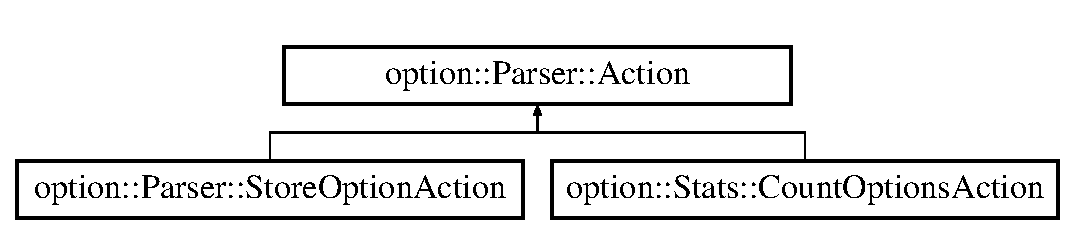
\includegraphics[height=2.000000cm]{structoption_1_1Parser_1_1Action}
\end{center}
\end{figure}
\subsection*{Public Member Functions}
\begin{DoxyCompactItemize}
\item 
virtual bool \hyperlink{structoption_1_1Parser_1_1Action_a176b5f783bb35eb015b6d2c09422457d}{perform} (\hyperlink{classoption_1_1Option}{Option} \&)
\begin{DoxyCompactList}\small\item\em Called by Parser\+::workhorse() for each \hyperlink{classoption_1_1Option}{Option} that has been successfully parsed (including unknown options if they have a \hyperlink{structoption_1_1Descriptor}{Descriptor} whose \hyperlink{structoption_1_1Descriptor_aa5d675dba0214a4abd73007ff163cc67}{Descriptor\+::check\+\_\+arg} does not return \hyperlink{namespaceoption_aee8c76a07877335762631491e7a5a1a9a9528e32563b795bd2930b12d0a5e382d}{A\+R\+G\+\_\+\+I\+L\+L\+E\+G\+AL}. \end{DoxyCompactList}\item 
virtual bool \hyperlink{structoption_1_1Parser_1_1Action_a3ec558b51e34d33d116f14587289e032}{finished} (int numargs, const char $\ast$$\ast$args)
\begin{DoxyCompactList}\small\item\em Called by Parser\+::workhorse() after finishing the parse. \end{DoxyCompactList}\end{DoxyCompactItemize}


\subsection{Member Function Documentation}
\mbox{\Hypertarget{structoption_1_1Parser_1_1Action_a3ec558b51e34d33d116f14587289e032}\label{structoption_1_1Parser_1_1Action_a3ec558b51e34d33d116f14587289e032}} 
\index{option\+::\+Parser\+::\+Action@{option\+::\+Parser\+::\+Action}!finished@{finished}}
\index{finished@{finished}!option\+::\+Parser\+::\+Action@{option\+::\+Parser\+::\+Action}}
\subsubsection{\texorpdfstring{finished()}{finished()}}
{\footnotesize\ttfamily virtual bool option\+::\+Parser\+::\+Action\+::finished (\begin{DoxyParamCaption}\item[{int}]{numargs,  }\item[{const char $\ast$$\ast$}]{args }\end{DoxyParamCaption})\hspace{0.3cm}{\ttfamily [inline]}, {\ttfamily [virtual]}}



Called by Parser\+::workhorse() after finishing the parse. 


\begin{DoxyParams}{Parameters}
{\em numargs} & the number of non-\/option arguments remaining \\
\hline
{\em args} & pointer to the first remaining non-\/option argument (if numargs $>$ 0).\\
\hline
\end{DoxyParams}
\begin{DoxyReturn}{Returns}
{\ttfamily false} iff a fatal error has occurred. 
\end{DoxyReturn}


Reimplemented in \hyperlink{classoption_1_1Parser_1_1StoreOptionAction_a617f675ef50a72ae36ce91f065bc8441}{option\+::\+Parser\+::\+Store\+Option\+Action}.

\mbox{\Hypertarget{structoption_1_1Parser_1_1Action_a176b5f783bb35eb015b6d2c09422457d}\label{structoption_1_1Parser_1_1Action_a176b5f783bb35eb015b6d2c09422457d}} 
\index{option\+::\+Parser\+::\+Action@{option\+::\+Parser\+::\+Action}!perform@{perform}}
\index{perform@{perform}!option\+::\+Parser\+::\+Action@{option\+::\+Parser\+::\+Action}}
\subsubsection{\texorpdfstring{perform()}{perform()}}
{\footnotesize\ttfamily virtual bool option\+::\+Parser\+::\+Action\+::perform (\begin{DoxyParamCaption}\item[{\hyperlink{classoption_1_1Option}{Option} \&}]{ }\end{DoxyParamCaption})\hspace{0.3cm}{\ttfamily [inline]}, {\ttfamily [virtual]}}



Called by Parser\+::workhorse() for each \hyperlink{classoption_1_1Option}{Option} that has been successfully parsed (including unknown options if they have a \hyperlink{structoption_1_1Descriptor}{Descriptor} whose \hyperlink{structoption_1_1Descriptor_aa5d675dba0214a4abd73007ff163cc67}{Descriptor\+::check\+\_\+arg} does not return \hyperlink{namespaceoption_aee8c76a07877335762631491e7a5a1a9a9528e32563b795bd2930b12d0a5e382d}{A\+R\+G\+\_\+\+I\+L\+L\+E\+G\+AL}. 

Returns {\ttfamily false} iff a fatal error has occured and the parse should be aborted. 

Reimplemented in \hyperlink{classoption_1_1Parser_1_1StoreOptionAction_a8931919fba5516377c202920db2b2f84}{option\+::\+Parser\+::\+Store\+Option\+Action}, and \hyperlink{classoption_1_1Stats_1_1CountOptionsAction_a29ab8a68d0a30736b99b4d2e5dece489}{option\+::\+Stats\+::\+Count\+Options\+Action}.



The documentation for this struct was generated from the following file\+:\begin{DoxyCompactItemize}
\item 
headers/\hyperlink{optionparser_8hpp}{optionparser.\+hpp}\end{DoxyCompactItemize}

\hypertarget{structArg}{}\section{Arg Struct Reference}
\label{structArg}\index{Arg@{Arg}}
Inheritance diagram for Arg\+:\begin{figure}[H]
\begin{center}
\leavevmode
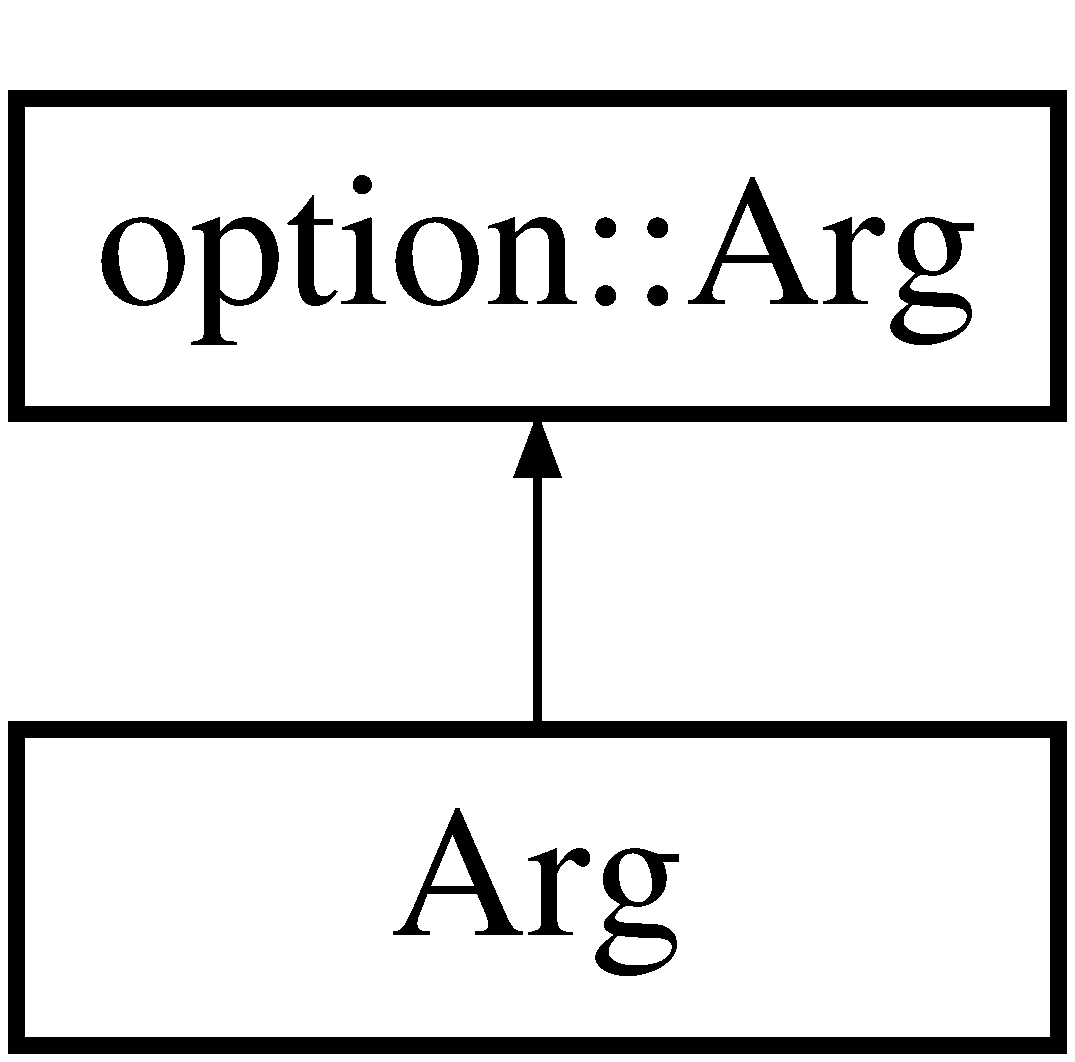
\includegraphics[height=2.000000cm]{structArg}
\end{center}
\end{figure}
\subsection*{Static Public Member Functions}
\begin{DoxyCompactItemize}
\item 
\mbox{\Hypertarget{structArg_ac02bc8cf3aec0a37643d1c4e72e53247}\label{structArg_ac02bc8cf3aec0a37643d1c4e72e53247}} 
static void {\bfseries print\+Error} (const char $\ast$msg1, const \hyperlink{classoption_1_1Option}{option\+::\+Option} \&opt, const char $\ast$msg2)
\item 
\mbox{\Hypertarget{structArg_a27e735e03504971f760309d1045b2602}\label{structArg_a27e735e03504971f760309d1045b2602}} 
static \hyperlink{namespaceoption_aee8c76a07877335762631491e7a5a1a9}{option\+::\+Arg\+Status} {\bfseries Unknown} (const \hyperlink{classoption_1_1Option}{option\+::\+Option} \&option, bool msg)
\item 
\mbox{\Hypertarget{structArg_a38aa6a5804c73eaacf5aa1feed10d495}\label{structArg_a38aa6a5804c73eaacf5aa1feed10d495}} 
static \hyperlink{namespaceoption_aee8c76a07877335762631491e7a5a1a9}{option\+::\+Arg\+Status} {\bfseries Numeric} (const \hyperlink{classoption_1_1Option}{option\+::\+Option} \&option, bool msg)
\item 
\mbox{\Hypertarget{structArg_a44445181427d8c2b953ed1ac8cf653f0}\label{structArg_a44445181427d8c2b953ed1ac8cf653f0}} 
static \hyperlink{namespaceoption_aee8c76a07877335762631491e7a5a1a9}{option\+::\+Arg\+Status} {\bfseries Non\+Empty} (const \hyperlink{classoption_1_1Option}{option\+::\+Option} \&option, bool msg)
\item 
\mbox{\Hypertarget{structArg_a7236f63281660f890f7ea961536f0b5e}\label{structArg_a7236f63281660f890f7ea961536f0b5e}} 
static \hyperlink{namespaceoption_aee8c76a07877335762631491e7a5a1a9}{option\+::\+Arg\+Status} {\bfseries File\+Name} (const \hyperlink{classoption_1_1Option}{option\+::\+Option} \&option, bool msg)
\end{DoxyCompactItemize}


The documentation for this struct was generated from the following file\+:\begin{DoxyCompactItemize}
\item 
sources/\hyperlink{main_8cpp}{main.\+cpp}\end{DoxyCompactItemize}

\hypertarget{structoption_1_1Arg}{}\section{option\+:\+:Arg Struct Reference}
\label{structoption_1_1Arg}\index{option\+::\+Arg@{option\+::\+Arg}}


Functions for checking the validity of option arguments.  




{\ttfamily \#include $<$optionparser.\+hpp$>$}

Inheritance diagram for option\+:\+:Arg\+:\begin{figure}[H]
\begin{center}
\leavevmode
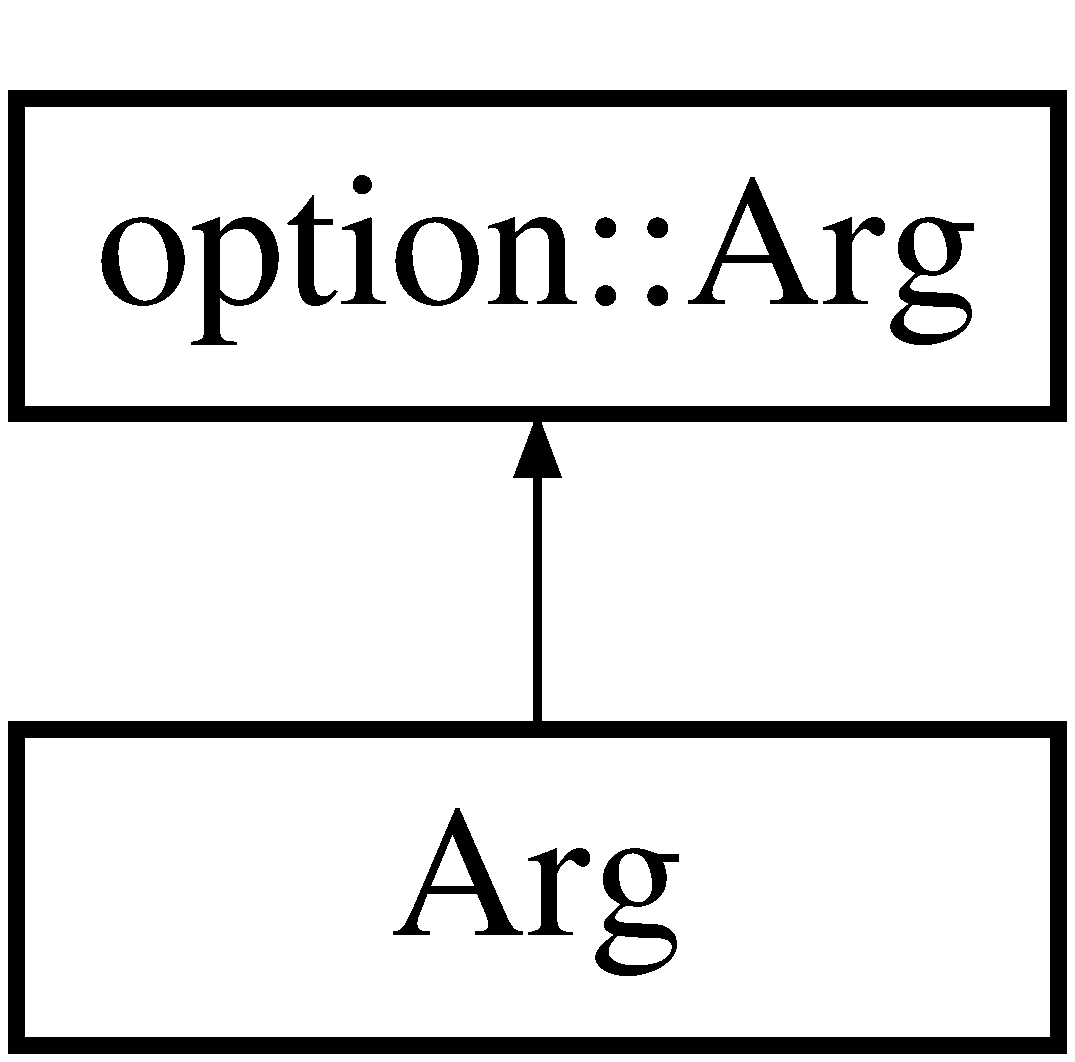
\includegraphics[height=2.000000cm]{structoption_1_1Arg}
\end{center}
\end{figure}
\subsection*{Static Public Member Functions}
\begin{DoxyCompactItemize}
\item 
\mbox{\Hypertarget{structoption_1_1Arg_a7fc01987899c91c6b6a1be5711a46e22}\label{structoption_1_1Arg_a7fc01987899c91c6b6a1be5711a46e22}} 
static \hyperlink{namespaceoption_aee8c76a07877335762631491e7a5a1a9}{Arg\+Status} \hyperlink{structoption_1_1Arg_a7fc01987899c91c6b6a1be5711a46e22}{None} (const \hyperlink{classoption_1_1Option}{Option} \&, bool)
\begin{DoxyCompactList}\small\item\em For options that don\textquotesingle{}t take an argument\+: Returns A\+R\+G\+\_\+\+N\+O\+NE. \end{DoxyCompactList}\item 
\mbox{\Hypertarget{structoption_1_1Arg_aadb5316ecbc9eb0a7f0019d14bf35ad0}\label{structoption_1_1Arg_aadb5316ecbc9eb0a7f0019d14bf35ad0}} 
static \hyperlink{namespaceoption_aee8c76a07877335762631491e7a5a1a9}{Arg\+Status} \hyperlink{structoption_1_1Arg_aadb5316ecbc9eb0a7f0019d14bf35ad0}{Optional} (const \hyperlink{classoption_1_1Option}{Option} \&option, bool)
\begin{DoxyCompactList}\small\item\em Returns A\+R\+G\+\_\+\+OK if the argument is attached and A\+R\+G\+\_\+\+I\+G\+N\+O\+RE otherwise. \end{DoxyCompactList}\end{DoxyCompactItemize}


\subsection{Detailed Description}
Functions for checking the validity of option arguments. 

Every \hyperlink{classoption_1_1Option}{Option} has such a function assigned in its \hyperlink{structoption_1_1Descriptor}{Descriptor}. 
\begin{DoxyCode}
Descriptor usage[] = \{ \{UNKNOWN, 0, \textcolor{stringliteral}{""}, \textcolor{stringliteral}{""}, \hyperlink{structoption_1_1Arg_a7fc01987899c91c6b6a1be5711a46e22}{Arg::None}, \textcolor{stringliteral}{""}\}, ... \};
\end{DoxyCode}


A Check\+Arg function has the following signature\+: 
\begin{DoxyCode}
\hyperlink{namespaceoption_aee8c76a07877335762631491e7a5a1a9}{ArgStatus} \hyperlink{namespaceoption_a4cdf403efae65e18bf850e2001b12a2a}{CheckArg}(\textcolor{keyword}{const} Option& option, \textcolor{keywordtype}{bool} msg); 
\end{DoxyCode}


It is used to check if a potential argument would be acceptable for the option. It will even be called if there is no argument. In that case {\ttfamily option.\+arg} will be {\ttfamily N\+U\+LL}.

If {\ttfamily msg} is {\ttfamily true} and the function determines that an argument is not acceptable and that this is a fatal error, it should output a message to the user before returning \hyperlink{namespaceoption_aee8c76a07877335762631491e7a5a1a9a9528e32563b795bd2930b12d0a5e382d}{A\+R\+G\+\_\+\+I\+L\+L\+E\+G\+AL}. If {\ttfamily msg} is {\ttfamily false} the function should remain silent (or you will get duplicate messages).

See \hyperlink{namespaceoption_aee8c76a07877335762631491e7a5a1a9}{Arg\+Status} for the meaning of the return values.

While you can provide your own functions, often the following pre-\/defined checks (which never return \hyperlink{namespaceoption_aee8c76a07877335762631491e7a5a1a9a9528e32563b795bd2930b12d0a5e382d}{A\+R\+G\+\_\+\+I\+L\+L\+E\+G\+AL}) will suffice\+:

\begin{DoxyItemize}
\item {\ttfamily \hyperlink{structoption_1_1Arg_a7fc01987899c91c6b6a1be5711a46e22}{Arg\+::\+None}} For options that don\textquotesingle{}t take an argument\+: Returns A\+R\+G\+\_\+\+N\+O\+NE. \item {\ttfamily \hyperlink{structoption_1_1Arg_aadb5316ecbc9eb0a7f0019d14bf35ad0}{Arg\+::\+Optional}} Returns A\+R\+G\+\_\+\+OK if the argument is attached and A\+R\+G\+\_\+\+I\+G\+N\+O\+RE otherwise.\end{DoxyItemize}
The following example code can serve as starting place for writing your own more complex Check\+Arg functions\+: 
\begin{DoxyCode}
\textcolor{keyword}{struct }\hyperlink{structArg}{Arg}: \textcolor{keyword}{public} \hyperlink{structoption_1_1Arg}{option::Arg}
\{
  \textcolor{keyword}{static} \textcolor{keywordtype}{void} printError(\textcolor{keyword}{const} \textcolor{keywordtype}{char}* msg1, \textcolor{keyword}{const} \hyperlink{classoption_1_1Option}{option::Option}& opt, \textcolor{keyword}{const} \textcolor{keywordtype}{char}* msg2)
  \{
    fprintf(stderr, \textcolor{stringliteral}{"ERROR: %s"}, msg1);
    fwrite(opt.\hyperlink{classoption_1_1Option_a02a76b4896abd22d0ba8514362261de9}{name}, opt.\hyperlink{classoption_1_1Option_a3aa2957b19ad5815873441b415d56050}{namelen}, 1, stderr);
    fprintf(stderr, \textcolor{stringliteral}{"%s"}, msg2);
  \}

  \textcolor{keyword}{static} \hyperlink{namespaceoption_aee8c76a07877335762631491e7a5a1a9}{option::ArgStatus} Unknown(\textcolor{keyword}{const} \hyperlink{classoption_1_1Option}{option::Option}& option, \textcolor{keywordtype}{bool} msg)
  \{
    \textcolor{keywordflow}{if} (msg) printError(\textcolor{stringliteral}{"Unknown option '"}, option, \textcolor{stringliteral}{"'\(\backslash\)n"});
    \textcolor{keywordflow}{return} \hyperlink{namespaceoption_aee8c76a07877335762631491e7a5a1a9a9528e32563b795bd2930b12d0a5e382d}{option::ARG\_ILLEGAL};
  \}

  \textcolor{keyword}{static} \hyperlink{namespaceoption_aee8c76a07877335762631491e7a5a1a9}{option::ArgStatus} Required(\textcolor{keyword}{const} \hyperlink{classoption_1_1Option}{option::Option}& option, \textcolor{keywordtype}{bool} msg)
  \{
    \textcolor{keywordflow}{if} (option.\hyperlink{classoption_1_1Option_a402be734987458364b0f473acae36238}{arg} != 0)
      \textcolor{keywordflow}{return} \hyperlink{namespaceoption_aee8c76a07877335762631491e7a5a1a9a445e08cb1747e5a22929e7ef2da43b55}{option::ARG\_OK};

    \textcolor{keywordflow}{if} (msg) printError(\textcolor{stringliteral}{"Option '"}, option, \textcolor{stringliteral}{"' requires an argument\(\backslash\)n"});
    \textcolor{keywordflow}{return} \hyperlink{namespaceoption_aee8c76a07877335762631491e7a5a1a9a9528e32563b795bd2930b12d0a5e382d}{option::ARG\_ILLEGAL};
  \}

  \textcolor{keyword}{static} \hyperlink{namespaceoption_aee8c76a07877335762631491e7a5a1a9}{option::ArgStatus} NonEmpty(\textcolor{keyword}{const} \hyperlink{classoption_1_1Option}{option::Option}& option, \textcolor{keywordtype}{bool} msg)
  \{
    \textcolor{keywordflow}{if} (option.\hyperlink{classoption_1_1Option_a402be734987458364b0f473acae36238}{arg} != 0 && option.\hyperlink{classoption_1_1Option_a402be734987458364b0f473acae36238}{arg}[0] != 0)
      \textcolor{keywordflow}{return} \hyperlink{namespaceoption_aee8c76a07877335762631491e7a5a1a9a445e08cb1747e5a22929e7ef2da43b55}{option::ARG\_OK};

    \textcolor{keywordflow}{if} (msg) printError(\textcolor{stringliteral}{"Option '"}, option, \textcolor{stringliteral}{"' requires a non-empty argument\(\backslash\)n"});
    \textcolor{keywordflow}{return} \hyperlink{namespaceoption_aee8c76a07877335762631491e7a5a1a9a9528e32563b795bd2930b12d0a5e382d}{option::ARG\_ILLEGAL};
  \}

  \textcolor{keyword}{static} \hyperlink{namespaceoption_aee8c76a07877335762631491e7a5a1a9}{option::ArgStatus} Numeric(\textcolor{keyword}{const} \hyperlink{classoption_1_1Option}{option::Option}& option, \textcolor{keywordtype}{bool} msg)
  \{
    \textcolor{keywordtype}{char}* endptr = 0;
    \textcolor{keywordflow}{if} (option.\hyperlink{classoption_1_1Option_a402be734987458364b0f473acae36238}{arg} != 0 && strtol(option.\hyperlink{classoption_1_1Option_a402be734987458364b0f473acae36238}{arg}, &endptr, 10))\{\};
    \textcolor{keywordflow}{if} (endptr != option.\hyperlink{classoption_1_1Option_a402be734987458364b0f473acae36238}{arg} && *endptr == 0)
      \textcolor{keywordflow}{return} \hyperlink{namespaceoption_aee8c76a07877335762631491e7a5a1a9a445e08cb1747e5a22929e7ef2da43b55}{option::ARG\_OK};

    \textcolor{keywordflow}{if} (msg) printError(\textcolor{stringliteral}{"Option '"}, option, \textcolor{stringliteral}{"' requires a numeric argument\(\backslash\)n"});
    \textcolor{keywordflow}{return} \hyperlink{namespaceoption_aee8c76a07877335762631491e7a5a1a9a9528e32563b795bd2930b12d0a5e382d}{option::ARG\_ILLEGAL};
  \}
\};
\end{DoxyCode}
 

The documentation for this struct was generated from the following file\+:\begin{DoxyCompactItemize}
\item 
headers/\hyperlink{optionparser_8hpp}{optionparser.\+hpp}\end{DoxyCompactItemize}

\hypertarget{classoption_1_1Stats_1_1CountOptionsAction}{}\section{option\+:\+:Stats\+:\+:Count\+Options\+Action Class Reference}
\label{classoption_1_1Stats_1_1CountOptionsAction}\index{option\+::\+Stats\+::\+Count\+Options\+Action@{option\+::\+Stats\+::\+Count\+Options\+Action}}
Inheritance diagram for option\+:\+:Stats\+:\+:Count\+Options\+Action\+:\begin{figure}[H]
\begin{center}
\leavevmode
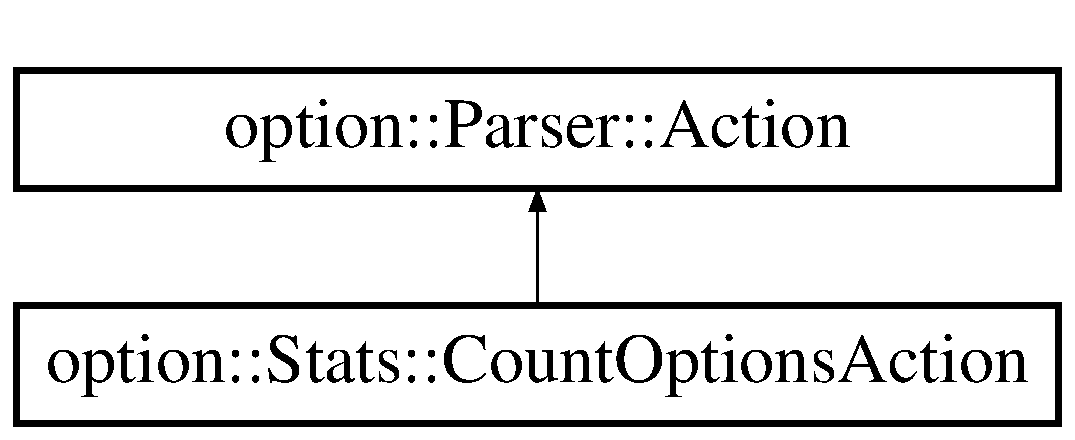
\includegraphics[height=2.000000cm]{classoption_1_1Stats_1_1CountOptionsAction}
\end{center}
\end{figure}
\subsection*{Public Member Functions}
\begin{DoxyCompactItemize}
\item 
\hyperlink{classoption_1_1Stats_1_1CountOptionsAction_a24a38b87ad129b0e12660bd2019ba284}{Count\+Options\+Action} (unsigned $\ast$buffer\+\_\+max\+\_\+)
\item 
bool \hyperlink{classoption_1_1Stats_1_1CountOptionsAction_a29ab8a68d0a30736b99b4d2e5dece489}{perform} (\hyperlink{classoption_1_1Option}{Option} \&)
\begin{DoxyCompactList}\small\item\em Called by Parser\+::workhorse() for each \hyperlink{classoption_1_1Option}{Option} that has been successfully parsed (including unknown options if they have a \hyperlink{structoption_1_1Descriptor}{Descriptor} whose \hyperlink{structoption_1_1Descriptor_aa5d675dba0214a4abd73007ff163cc67}{Descriptor\+::check\+\_\+arg} does not return \hyperlink{namespaceoption_aee8c76a07877335762631491e7a5a1a9a9528e32563b795bd2930b12d0a5e382d}{A\+R\+G\+\_\+\+I\+L\+L\+E\+G\+AL}. \end{DoxyCompactList}\end{DoxyCompactItemize}


\subsection{Constructor \& Destructor Documentation}
\mbox{\Hypertarget{classoption_1_1Stats_1_1CountOptionsAction_a24a38b87ad129b0e12660bd2019ba284}\label{classoption_1_1Stats_1_1CountOptionsAction_a24a38b87ad129b0e12660bd2019ba284}} 
\index{option\+::\+Stats\+::\+Count\+Options\+Action@{option\+::\+Stats\+::\+Count\+Options\+Action}!Count\+Options\+Action@{Count\+Options\+Action}}
\index{Count\+Options\+Action@{Count\+Options\+Action}!option\+::\+Stats\+::\+Count\+Options\+Action@{option\+::\+Stats\+::\+Count\+Options\+Action}}
\subsubsection{\texorpdfstring{Count\+Options\+Action()}{CountOptionsAction()}}
{\footnotesize\ttfamily option\+::\+Stats\+::\+Count\+Options\+Action\+::\+Count\+Options\+Action (\begin{DoxyParamCaption}\item[{unsigned $\ast$}]{buffer\+\_\+max\+\_\+ }\end{DoxyParamCaption})\hspace{0.3cm}{\ttfamily [inline]}}

Creates a new \hyperlink{classoption_1_1Stats_1_1CountOptionsAction}{Count\+Options\+Action} that will increase {\ttfamily $\ast$buffer\+\_\+max\+\_\+} for each parsed \hyperlink{classoption_1_1Option}{Option}. 

\subsection{Member Function Documentation}
\mbox{\Hypertarget{classoption_1_1Stats_1_1CountOptionsAction_a29ab8a68d0a30736b99b4d2e5dece489}\label{classoption_1_1Stats_1_1CountOptionsAction_a29ab8a68d0a30736b99b4d2e5dece489}} 
\index{option\+::\+Stats\+::\+Count\+Options\+Action@{option\+::\+Stats\+::\+Count\+Options\+Action}!perform@{perform}}
\index{perform@{perform}!option\+::\+Stats\+::\+Count\+Options\+Action@{option\+::\+Stats\+::\+Count\+Options\+Action}}
\subsubsection{\texorpdfstring{perform()}{perform()}}
{\footnotesize\ttfamily bool option\+::\+Stats\+::\+Count\+Options\+Action\+::perform (\begin{DoxyParamCaption}\item[{\hyperlink{classoption_1_1Option}{Option} \&}]{ }\end{DoxyParamCaption})\hspace{0.3cm}{\ttfamily [inline]}, {\ttfamily [virtual]}}



Called by Parser\+::workhorse() for each \hyperlink{classoption_1_1Option}{Option} that has been successfully parsed (including unknown options if they have a \hyperlink{structoption_1_1Descriptor}{Descriptor} whose \hyperlink{structoption_1_1Descriptor_aa5d675dba0214a4abd73007ff163cc67}{Descriptor\+::check\+\_\+arg} does not return \hyperlink{namespaceoption_aee8c76a07877335762631491e7a5a1a9a9528e32563b795bd2930b12d0a5e382d}{A\+R\+G\+\_\+\+I\+L\+L\+E\+G\+AL}. 

Returns {\ttfamily false} iff a fatal error has occured and the parse should be aborted. 

Reimplemented from \hyperlink{structoption_1_1Parser_1_1Action_a176b5f783bb35eb015b6d2c09422457d}{option\+::\+Parser\+::\+Action}.



The documentation for this class was generated from the following file\+:\begin{DoxyCompactItemize}
\item 
headers/\hyperlink{optionparser_8hpp}{optionparser.\+hpp}\end{DoxyCompactItemize}

\hypertarget{structoption_1_1Descriptor}{}\section{option\+:\+:Descriptor Struct Reference}
\label{structoption_1_1Descriptor}\index{option\+::\+Descriptor@{option\+::\+Descriptor}}


Describes an option, its help text (usage) and how it should be parsed.  




{\ttfamily \#include $<$optionparser.\+hpp$>$}

\subsection*{Public Attributes}
\begin{DoxyCompactItemize}
\item 
const unsigned \hyperlink{structoption_1_1Descriptor_a1fee8ac44f529c99ac2b1149b4c391b1}{index}
\begin{DoxyCompactList}\small\item\em Index of this option\textquotesingle{}s linked list in the array filled in by the parser. \end{DoxyCompactList}\item 
const int \hyperlink{structoption_1_1Descriptor_a1b220dabd8aad075fa441a80f9b9343c}{type}
\begin{DoxyCompactList}\small\item\em Used to distinguish between options with the same \hyperlink{structoption_1_1Descriptor_a1fee8ac44f529c99ac2b1149b4c391b1}{index}. See \hyperlink{structoption_1_1Descriptor_a1fee8ac44f529c99ac2b1149b4c391b1}{index} for details. \end{DoxyCompactList}\item 
const char $\ast$const \hyperlink{structoption_1_1Descriptor_a0dba4ccca59c19d6ed4081391fca5adb}{shortopt}
\begin{DoxyCompactList}\small\item\em Each char in this string will be accepted as a short option character. \end{DoxyCompactList}\item 
const char $\ast$const \hyperlink{structoption_1_1Descriptor_a470c449dfa894c9bfda2dae026142b4b}{longopt}
\begin{DoxyCompactList}\small\item\em The long option name (without the leading {\ttfamily --} ). \end{DoxyCompactList}\item 
const \hyperlink{namespaceoption_a4cdf403efae65e18bf850e2001b12a2a}{Check\+Arg} \hyperlink{structoption_1_1Descriptor_aa5d675dba0214a4abd73007ff163cc67}{check\+\_\+arg}
\begin{DoxyCompactList}\small\item\em For each option that matches \hyperlink{structoption_1_1Descriptor_a0dba4ccca59c19d6ed4081391fca5adb}{shortopt} or \hyperlink{structoption_1_1Descriptor_a470c449dfa894c9bfda2dae026142b4b}{longopt} this function will be called to check a potential argument to the option. \end{DoxyCompactList}\item 
const char $\ast$ \hyperlink{structoption_1_1Descriptor_a9045b19311533e1b8a08645d57149c79}{help}
\begin{DoxyCompactList}\small\item\em The usage text associated with the options in this \hyperlink{structoption_1_1Descriptor}{Descriptor}. \end{DoxyCompactList}\end{DoxyCompactItemize}


\subsection{Detailed Description}
Describes an option, its help text (usage) and how it should be parsed. 

The main input when constructing an \hyperlink{classoption_1_1Parser}{option\+::\+Parser} is an array of Descriptors.

\begin{DoxyParagraph}{Example\+:}

\begin{DoxyCode}
\textcolor{keyword}{enum} OptionIndex \{CREATE, ...\};
\textcolor{keyword}{enum} OptionType \{DISABLE, ENABLE, OTHER\};

\textcolor{keyword}{const} \hyperlink{structoption_1_1Descriptor}{option::Descriptor} usage[] = \{
  \{ CREATE,                                            \textcolor{comment}{// index}
    OTHER,                                             \textcolor{comment}{// type}
    \textcolor{stringliteral}{"c"},                                               \textcolor{comment}{// shortopt}
    \textcolor{stringliteral}{"create"},                                          \textcolor{comment}{// longopt}
    \hyperlink{structoption_1_1Arg_a7fc01987899c91c6b6a1be5711a46e22}{Arg::None},                                         \textcolor{comment}{// check\_arg}
    \textcolor{stringliteral}{"--create  Tells the program to create something."} \textcolor{comment}{// help}
  \}
  , ...
\};
\end{DoxyCode}
 
\end{DoxyParagraph}


\subsection{Member Data Documentation}
\mbox{\Hypertarget{structoption_1_1Descriptor_aa5d675dba0214a4abd73007ff163cc67}\label{structoption_1_1Descriptor_aa5d675dba0214a4abd73007ff163cc67}} 
\index{option\+::\+Descriptor@{option\+::\+Descriptor}!check\+\_\+arg@{check\+\_\+arg}}
\index{check\+\_\+arg@{check\+\_\+arg}!option\+::\+Descriptor@{option\+::\+Descriptor}}
\subsubsection{\texorpdfstring{check\+\_\+arg}{check\_arg}}
{\footnotesize\ttfamily const \hyperlink{namespaceoption_a4cdf403efae65e18bf850e2001b12a2a}{Check\+Arg} option\+::\+Descriptor\+::check\+\_\+arg}



For each option that matches \hyperlink{structoption_1_1Descriptor_a0dba4ccca59c19d6ed4081391fca5adb}{shortopt} or \hyperlink{structoption_1_1Descriptor_a470c449dfa894c9bfda2dae026142b4b}{longopt} this function will be called to check a potential argument to the option. 

This function will be called even if there is no potential argument. In that case it will be passed {\ttfamily N\+U\+LL} as {\ttfamily arg} parameter. Do not confuse this with the empty string.

See \hyperlink{namespaceoption_a4cdf403efae65e18bf850e2001b12a2a}{Check\+Arg} for more information. \mbox{\Hypertarget{structoption_1_1Descriptor_a9045b19311533e1b8a08645d57149c79}\label{structoption_1_1Descriptor_a9045b19311533e1b8a08645d57149c79}} 
\index{option\+::\+Descriptor@{option\+::\+Descriptor}!help@{help}}
\index{help@{help}!option\+::\+Descriptor@{option\+::\+Descriptor}}
\subsubsection{\texorpdfstring{help}{help}}
{\footnotesize\ttfamily const char$\ast$ option\+::\+Descriptor\+::help}



The usage text associated with the options in this \hyperlink{structoption_1_1Descriptor}{Descriptor}. 

You can use \hyperlink{namespaceoption_afc8bb7e040a98a0b33ff1ce9da1be0d1}{option\+::print\+Usage()} to format your usage message based on the {\ttfamily help} texts. You can use dummy Descriptors where \hyperlink{structoption_1_1Descriptor_a0dba4ccca59c19d6ed4081391fca5adb}{shortopt} and \hyperlink{structoption_1_1Descriptor_a470c449dfa894c9bfda2dae026142b4b}{longopt} are both the empty string to add text to the usage that is not related to a specific option.

See \hyperlink{namespaceoption_afc8bb7e040a98a0b33ff1ce9da1be0d1}{option\+::print\+Usage()} for special formatting characters you can use in {\ttfamily help} to get a column layout.

\begin{DoxyAttention}{Attention}
Must be U\+T\+F-\/8-\/encoded. If your compiler supports C++11 you can use the \char`\"{}u8\char`\"{} prefix to make sure string literals are properly encoded. 
\end{DoxyAttention}
\mbox{\Hypertarget{structoption_1_1Descriptor_a1fee8ac44f529c99ac2b1149b4c391b1}\label{structoption_1_1Descriptor_a1fee8ac44f529c99ac2b1149b4c391b1}} 
\index{option\+::\+Descriptor@{option\+::\+Descriptor}!index@{index}}
\index{index@{index}!option\+::\+Descriptor@{option\+::\+Descriptor}}
\subsubsection{\texorpdfstring{index}{index}}
{\footnotesize\ttfamily const unsigned option\+::\+Descriptor\+::index}



Index of this option\textquotesingle{}s linked list in the array filled in by the parser. 

Command line options whose Descriptors have the same index will end up in the same linked list in the order in which they appear on the command line. If you have multiple long option aliases that refer to the same option, give their descriptors the same {\ttfamily index}.

If you have options that mean exactly opposite things (e.\+g. {\ttfamily --enable-\/foo} and {\ttfamily --disable-\/foo} ), you should also give them the same {\ttfamily index}, but distinguish them through different values for \hyperlink{structoption_1_1Descriptor_a1b220dabd8aad075fa441a80f9b9343c}{type}. That way they end up in the same list and you can just take the last element of the list and use its type. This way you get the usual behaviour where switches later on the command line override earlier ones without having to code it manually.

\begin{DoxyParagraph}{Tip\+:}
Use an enum rather than plain ints for better readability, as shown in the example at \hyperlink{structoption_1_1Descriptor}{Descriptor}. 
\end{DoxyParagraph}
\mbox{\Hypertarget{structoption_1_1Descriptor_a470c449dfa894c9bfda2dae026142b4b}\label{structoption_1_1Descriptor_a470c449dfa894c9bfda2dae026142b4b}} 
\index{option\+::\+Descriptor@{option\+::\+Descriptor}!longopt@{longopt}}
\index{longopt@{longopt}!option\+::\+Descriptor@{option\+::\+Descriptor}}
\subsubsection{\texorpdfstring{longopt}{longopt}}
{\footnotesize\ttfamily const char$\ast$ const option\+::\+Descriptor\+::longopt}



The long option name (without the leading {\ttfamily --} ). 

If this \hyperlink{structoption_1_1Descriptor}{Descriptor} should not have a long option name, use the empty string \char`\"{}\char`\"{}. N\+U\+LL is not permitted here!

While \hyperlink{structoption_1_1Descriptor_a0dba4ccca59c19d6ed4081391fca5adb}{shortopt} allows multiple short option characters, each \hyperlink{structoption_1_1Descriptor}{Descriptor} can have only a single long option name. If you have multiple long option names referring to the same option use separate Descriptors that have the same \hyperlink{structoption_1_1Descriptor_a1fee8ac44f529c99ac2b1149b4c391b1}{index} and \hyperlink{structoption_1_1Descriptor_a1b220dabd8aad075fa441a80f9b9343c}{type}. You may repeat short option characters in such an alias \hyperlink{structoption_1_1Descriptor}{Descriptor} but there\textquotesingle{}s no need to.

\begin{DoxyParagraph}{Dummy Descriptors\+:}
You can use dummy Descriptors with an empty string for both \hyperlink{structoption_1_1Descriptor_a0dba4ccca59c19d6ed4081391fca5adb}{shortopt} and \hyperlink{structoption_1_1Descriptor_a470c449dfa894c9bfda2dae026142b4b}{longopt} to add text to the usage that is not related to a specific option. See \hyperlink{structoption_1_1Descriptor_a9045b19311533e1b8a08645d57149c79}{help}. The first dummy \hyperlink{structoption_1_1Descriptor}{Descriptor} will be used for unknown options (see below).
\end{DoxyParagraph}
\begin{DoxyParagraph}{Unknown Option Descriptor\+:}
The first dummy \hyperlink{structoption_1_1Descriptor}{Descriptor} in the list of Descriptors, whose \hyperlink{structoption_1_1Descriptor_a0dba4ccca59c19d6ed4081391fca5adb}{shortopt} and \hyperlink{structoption_1_1Descriptor_a470c449dfa894c9bfda2dae026142b4b}{longopt} are both the empty string, will be used as the \hyperlink{structoption_1_1Descriptor}{Descriptor} for unknown options. An unknown option is a string in the argument vector that is not a lone minus {\ttfamily \textquotesingle{}-\/\textquotesingle{}} but starts with a minus character and does not match any \hyperlink{structoption_1_1Descriptor}{Descriptor}\textquotesingle{}s \hyperlink{structoption_1_1Descriptor_a0dba4ccca59c19d6ed4081391fca5adb}{shortopt} or \hyperlink{structoption_1_1Descriptor_a470c449dfa894c9bfda2dae026142b4b}{longopt}. ~\newline
Note that the dummy descriptor\textquotesingle{}s \hyperlink{structoption_1_1Descriptor_aa5d675dba0214a4abd73007ff163cc67}{check\+\_\+arg} function {\itshape will} be called and its return value will be evaluated as usual. I.\+e. if it returns \hyperlink{namespaceoption_aee8c76a07877335762631491e7a5a1a9a9528e32563b795bd2930b12d0a5e382d}{A\+R\+G\+\_\+\+I\+L\+L\+E\+G\+AL} the parsing will be aborted with {\ttfamily \hyperlink{classoption_1_1Parser_a2caa149140067b4d13e4d7a104bb3090}{Parser\+::error()}==true}. ~\newline
if {\ttfamily check\+\_\+arg} does not return \hyperlink{namespaceoption_aee8c76a07877335762631491e7a5a1a9a9528e32563b795bd2930b12d0a5e382d}{A\+R\+G\+\_\+\+I\+L\+L\+E\+G\+AL} the descriptor\textquotesingle{}s \hyperlink{structoption_1_1Descriptor_a1fee8ac44f529c99ac2b1149b4c391b1}{index} {\itshape will} be used to pick the linked list into which to put the unknown option. ~\newline
If there is no dummy descriptor, unknown options will be dropped silently. 
\end{DoxyParagraph}
\mbox{\Hypertarget{structoption_1_1Descriptor_a0dba4ccca59c19d6ed4081391fca5adb}\label{structoption_1_1Descriptor_a0dba4ccca59c19d6ed4081391fca5adb}} 
\index{option\+::\+Descriptor@{option\+::\+Descriptor}!shortopt@{shortopt}}
\index{shortopt@{shortopt}!option\+::\+Descriptor@{option\+::\+Descriptor}}
\subsubsection{\texorpdfstring{shortopt}{shortopt}}
{\footnotesize\ttfamily const char$\ast$ const option\+::\+Descriptor\+::shortopt}



Each char in this string will be accepted as a short option character. 

The string must not include the minus character {\ttfamily \textquotesingle{}-\/\textquotesingle{}} or you\textquotesingle{}ll get undefined behaviour.

If this \hyperlink{structoption_1_1Descriptor}{Descriptor} should not have short option characters, use the empty string \char`\"{}\char`\"{}. N\+U\+LL is not permitted here!

See \hyperlink{structoption_1_1Descriptor_a470c449dfa894c9bfda2dae026142b4b}{longopt} for more information. \mbox{\Hypertarget{structoption_1_1Descriptor_a1b220dabd8aad075fa441a80f9b9343c}\label{structoption_1_1Descriptor_a1b220dabd8aad075fa441a80f9b9343c}} 
\index{option\+::\+Descriptor@{option\+::\+Descriptor}!type@{type}}
\index{type@{type}!option\+::\+Descriptor@{option\+::\+Descriptor}}
\subsubsection{\texorpdfstring{type}{type}}
{\footnotesize\ttfamily const int option\+::\+Descriptor\+::type}



Used to distinguish between options with the same \hyperlink{structoption_1_1Descriptor_a1fee8ac44f529c99ac2b1149b4c391b1}{index}. See \hyperlink{structoption_1_1Descriptor_a1fee8ac44f529c99ac2b1149b4c391b1}{index} for details. 

It is recommended that you use an enum rather than a plain int to make your code more readable. 

The documentation for this struct was generated from the following file\+:\begin{DoxyCompactItemize}
\item 
headers/\hyperlink{optionparser_8hpp}{optionparser.\+hpp}\end{DoxyCompactItemize}

\hypertarget{classEnglish}{}\section{English Class Reference}
\label{classEnglish}\index{English@{English}}
Inheritance diagram for English\+:\begin{figure}[H]
\begin{center}
\leavevmode
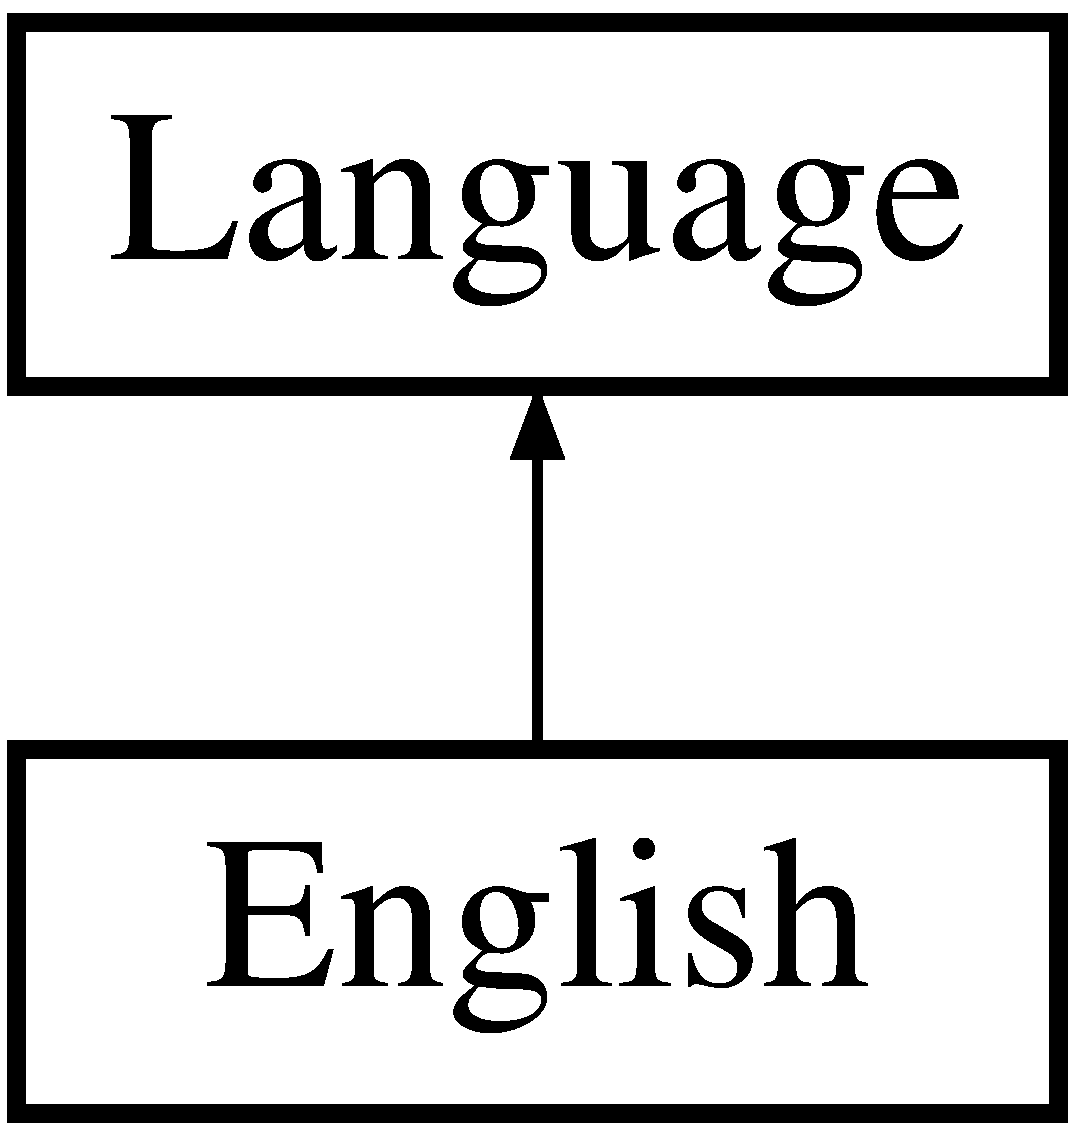
\includegraphics[height=2.000000cm]{classEnglish}
\end{center}
\end{figure}


The documentation for this class was generated from the following file\+:\begin{DoxyCompactItemize}
\item 
headers/\hyperlink{Language_8hpp}{Language.\+hpp}\end{DoxyCompactItemize}

\hypertarget{classFileManager}{}\section{File\+Manager Class Reference}
\label{classFileManager}\index{File\+Manager@{File\+Manager}}
\subsection*{Public Member Functions}
\begin{DoxyCompactItemize}
\item 
\hyperlink{classFileManager_a40ecb9b4c441c5108e25814d8d40824a}{File\+Manager} (string)
\item 
\hyperlink{classFileManager_abaed33b5b0c13b8a597db9335a1aacfa}{$\sim$\+File\+Manager} ()
\item 
\mbox{\Hypertarget{classFileManager_ab424d7f507a8804d7b8b8557fe481f46}\label{classFileManager_ab424d7f507a8804d7b8b8557fe481f46}} 
bool {\bfseries is\+\_\+open} ()
\item 
list$<$ string $>$ \hyperlink{classFileManager_abd1d0f98cb32a54435e491f876f73d14}{parse\+Lines} ()
\item 
int \hyperlink{classFileManager_a2ad30e54df4ffd2ca94b316ef43e1b1f}{save\+Lines} (list$<$ string $>$)
\item 
map$<$ char, double $>$ \hyperlink{classFileManager_afb8f7a73be3a7392fc822253aa554531}{parse\+Frequencies} ()
\item 
string \hyperlink{classFileManager_a92cce9f1145aaa39a52f4b991850d741}{text\+Only} ()
\end{DoxyCompactItemize}


\subsection{Constructor \& Destructor Documentation}
\mbox{\Hypertarget{classFileManager_a40ecb9b4c441c5108e25814d8d40824a}\label{classFileManager_a40ecb9b4c441c5108e25814d8d40824a}} 
\index{File\+Manager@{File\+Manager}!File\+Manager@{File\+Manager}}
\index{File\+Manager@{File\+Manager}!File\+Manager@{File\+Manager}}
\subsubsection{\texorpdfstring{File\+Manager()}{FileManager()}}
{\footnotesize\ttfamily File\+Manager\+::\+File\+Manager (\begin{DoxyParamCaption}\item[{string}]{file\+Name }\end{DoxyParamCaption})}

Constructor to safely open a file.


\begin{DoxyParams}{Parameters}
{\em file\+Name} & U\+RI to file \\
\hline
\end{DoxyParams}
\mbox{\Hypertarget{classFileManager_abaed33b5b0c13b8a597db9335a1aacfa}\label{classFileManager_abaed33b5b0c13b8a597db9335a1aacfa}} 
\index{File\+Manager@{File\+Manager}!````~File\+Manager@{$\sim$\+File\+Manager}}
\index{````~File\+Manager@{$\sim$\+File\+Manager}!File\+Manager@{File\+Manager}}
\subsubsection{\texorpdfstring{$\sim$\+File\+Manager()}{~FileManager()}}
{\footnotesize\ttfamily File\+Manager\+::$\sim$\+File\+Manager (\begin{DoxyParamCaption}{ }\end{DoxyParamCaption})}

Destructor ensures that the file is safely closed. 

\subsection{Member Function Documentation}
\mbox{\Hypertarget{classFileManager_afb8f7a73be3a7392fc822253aa554531}\label{classFileManager_afb8f7a73be3a7392fc822253aa554531}} 
\index{File\+Manager@{File\+Manager}!parse\+Frequencies@{parse\+Frequencies}}
\index{parse\+Frequencies@{parse\+Frequencies}!File\+Manager@{File\+Manager}}
\subsubsection{\texorpdfstring{parse\+Frequencies()}{parseFrequencies()}}
{\footnotesize\ttfamily map$<$ char, double $>$ File\+Manager\+::parse\+Frequencies (\begin{DoxyParamCaption}{ }\end{DoxyParamCaption})}

\begin{DoxyReturn}{Returns}
a map of chars and the recorded frequencies. 
\end{DoxyReturn}
\mbox{\Hypertarget{classFileManager_abd1d0f98cb32a54435e491f876f73d14}\label{classFileManager_abd1d0f98cb32a54435e491f876f73d14}} 
\index{File\+Manager@{File\+Manager}!parse\+Lines@{parse\+Lines}}
\index{parse\+Lines@{parse\+Lines}!File\+Manager@{File\+Manager}}
\subsubsection{\texorpdfstring{parse\+Lines()}{parseLines()}}
{\footnotesize\ttfamily list$<$ string $>$ File\+Manager\+::parse\+Lines (\begin{DoxyParamCaption}{ }\end{DoxyParamCaption})}

\begin{DoxyReturn}{Returns}
The file\textquotesingle{}s lines as a list of strings. 
\end{DoxyReturn}
\mbox{\Hypertarget{classFileManager_a2ad30e54df4ffd2ca94b316ef43e1b1f}\label{classFileManager_a2ad30e54df4ffd2ca94b316ef43e1b1f}} 
\index{File\+Manager@{File\+Manager}!save\+Lines@{save\+Lines}}
\index{save\+Lines@{save\+Lines}!File\+Manager@{File\+Manager}}
\subsubsection{\texorpdfstring{save\+Lines()}{saveLines()}}
{\footnotesize\ttfamily int File\+Manager\+::save\+Lines (\begin{DoxyParamCaption}\item[{list$<$ string $>$}]{lines }\end{DoxyParamCaption})}

Writes out a list of strings each on a new line.


\begin{DoxyParams}{Parameters}
{\em lines} & List of string to write. \\
\hline
\end{DoxyParams}
\begin{DoxyReturn}{Returns}
count of lines saved. 
\end{DoxyReturn}
\mbox{\Hypertarget{classFileManager_a92cce9f1145aaa39a52f4b991850d741}\label{classFileManager_a92cce9f1145aaa39a52f4b991850d741}} 
\index{File\+Manager@{File\+Manager}!text\+Only@{text\+Only}}
\index{text\+Only@{text\+Only}!File\+Manager@{File\+Manager}}
\subsubsection{\texorpdfstring{text\+Only()}{textOnly()}}
{\footnotesize\ttfamily string File\+Manager\+::text\+Only (\begin{DoxyParamCaption}{ }\end{DoxyParamCaption})}

\begin{DoxyReturn}{Returns}
The file\textquotesingle{}s lines as a single cleaned string 
\end{DoxyReturn}


The documentation for this class was generated from the following files\+:\begin{DoxyCompactItemize}
\item 
headers/\hyperlink{FileManager_8hpp}{File\+Manager.\+hpp}\item 
sources/File\+Manager.\+cpp\end{DoxyCompactItemize}

\hypertarget{classFrequency}{}\section{Frequency Class Reference}
\label{classFrequency}\index{Frequency@{Frequency}}
\subsection*{Public Member Functions}
\begin{DoxyCompactItemize}
\item 
\hyperlink{classFrequency_aee3a222d9a2c90ed28f3e08c20a661f3}{Frequency} (map$<$ char, double $>$, int)
\item 
\mbox{\Hypertarget{classFrequency_a39b7092591845fc4d32c51849c8b69cc}\label{classFrequency_a39b7092591845fc4d32c51849c8b69cc}} 
map$<$ char, double $>$ {\bfseries get\+Symbol\+Frequency} ()
\item 
\mbox{\Hypertarget{classFrequency_aebdcb9e2e49f7ecfb29c0ffb287eb8d2}\label{classFrequency_aebdcb9e2e49f7ecfb29c0ffb287eb8d2}} 
double {\bfseries get\+Symbol\+Frequency} (char)
\item 
\hyperlink{classRelFrequency}{Rel\+Frequency} \hyperlink{classFrequency_ad26f1ea2a3952447a6188d73cd26ca16}{get\+Relative\+Frequency} ()
\item 
\mbox{\Hypertarget{classFrequency_a4a55e109f83877daf7c4594f7a876d3f}\label{classFrequency_a4a55e109f83877daf7c4594f7a876d3f}} 
void {\bfseries print\+Frequencies} ()
\item 
\mbox{\Hypertarget{classFrequency_a76eb9ce63ed4658fbf6888e29414eb02}\label{classFrequency_a76eb9ce63ed4658fbf6888e29414eb02}} 
double {\bfseries compare} (\hyperlink{classFrequency}{Frequency})
\end{DoxyCompactItemize}
\subsection*{Static Public Member Functions}
\begin{DoxyCompactItemize}
\item 
static \hyperlink{classFrequency}{Frequency} \hyperlink{classFrequency_afa743a740aba09aa200406693c11afe8}{Frequency\+From\+C\+SV} (string)
\item 
static \hyperlink{classFrequency}{Frequency} \hyperlink{classFrequency_a1f7df4dabf9cdf839f9884ee844c6752}{Frequency\+From\+String} (string)
\item 
static \hyperlink{classFrequency}{Frequency} \hyperlink{classFrequency_ae46fea585785720e124b45643914f4c6}{Frequency\+From\+File} (string)
\end{DoxyCompactItemize}


\subsection{Constructor \& Destructor Documentation}
\mbox{\Hypertarget{classFrequency_aee3a222d9a2c90ed28f3e08c20a661f3}\label{classFrequency_aee3a222d9a2c90ed28f3e08c20a661f3}} 
\index{Frequency@{Frequency}!Frequency@{Frequency}}
\index{Frequency@{Frequency}!Frequency@{Frequency}}
\subsubsection{\texorpdfstring{Frequency()}{Frequency()}}
{\footnotesize\ttfamily Frequency\+::\+Frequency (\begin{DoxyParamCaption}\item[{map$<$ char, double $>$}]{F,  }\item[{int}]{T }\end{DoxyParamCaption})}

Constructor


\begin{DoxyParams}{Parameters}
{\em F} & Map between characters and their frequencies \\
\hline
{\em T} & Total characters in text \\
\hline
\end{DoxyParams}


\subsection{Member Function Documentation}
\mbox{\Hypertarget{classFrequency_afa743a740aba09aa200406693c11afe8}\label{classFrequency_afa743a740aba09aa200406693c11afe8}} 
\index{Frequency@{Frequency}!Frequency\+From\+C\+SV@{Frequency\+From\+C\+SV}}
\index{Frequency\+From\+C\+SV@{Frequency\+From\+C\+SV}!Frequency@{Frequency}}
\subsubsection{\texorpdfstring{Frequency\+From\+C\+S\+V()}{FrequencyFromCSV()}}
{\footnotesize\ttfamily \hyperlink{classFrequency}{Frequency} Frequency\+::\+Frequency\+From\+C\+SV (\begin{DoxyParamCaption}\item[{string}]{file }\end{DoxyParamCaption})\hspace{0.3cm}{\ttfamily [static]}}

Loads a previously saved frequency from a C\+SV file.


\begin{DoxyParams}{Parameters}
{\em file} & U\+RI of file \\
\hline
\end{DoxyParams}
\mbox{\Hypertarget{classFrequency_ae46fea585785720e124b45643914f4c6}\label{classFrequency_ae46fea585785720e124b45643914f4c6}} 
\index{Frequency@{Frequency}!Frequency\+From\+File@{Frequency\+From\+File}}
\index{Frequency\+From\+File@{Frequency\+From\+File}!Frequency@{Frequency}}
\subsubsection{\texorpdfstring{Frequency\+From\+File()}{FrequencyFromFile()}}
{\footnotesize\ttfamily \hyperlink{classFrequency}{Frequency} Frequency\+::\+Frequency\+From\+File (\begin{DoxyParamCaption}\item[{string}]{file }\end{DoxyParamCaption})\hspace{0.3cm}{\ttfamily [static]}}

Read a file and counts symbol frequencies.


\begin{DoxyParams}{Parameters}
{\em file} & U\+RI of file \\
\hline
\end{DoxyParams}
\mbox{\Hypertarget{classFrequency_a1f7df4dabf9cdf839f9884ee844c6752}\label{classFrequency_a1f7df4dabf9cdf839f9884ee844c6752}} 
\index{Frequency@{Frequency}!Frequency\+From\+String@{Frequency\+From\+String}}
\index{Frequency\+From\+String@{Frequency\+From\+String}!Frequency@{Frequency}}
\subsubsection{\texorpdfstring{Frequency\+From\+String()}{FrequencyFromString()}}
{\footnotesize\ttfamily \hyperlink{classFrequency}{Frequency} Frequency\+::\+Frequency\+From\+String (\begin{DoxyParamCaption}\item[{string}]{cipher\+Text }\end{DoxyParamCaption})\hspace{0.3cm}{\ttfamily [static]}}

Named constructor


\begin{DoxyParams}{Parameters}
{\em cipher\+Text} & String of text to analyse for symbol frequencies \\
\hline
\end{DoxyParams}
\mbox{\Hypertarget{classFrequency_ad26f1ea2a3952447a6188d73cd26ca16}\label{classFrequency_ad26f1ea2a3952447a6188d73cd26ca16}} 
\index{Frequency@{Frequency}!get\+Relative\+Frequency@{get\+Relative\+Frequency}}
\index{get\+Relative\+Frequency@{get\+Relative\+Frequency}!Frequency@{Frequency}}
\subsubsection{\texorpdfstring{get\+Relative\+Frequency()}{getRelativeFrequency()}}
{\footnotesize\ttfamily \hyperlink{classRelFrequency}{Rel\+Frequency} Frequency\+::get\+Relative\+Frequency (\begin{DoxyParamCaption}{ }\end{DoxyParamCaption})}

Turns an absolute frequency set into it\textquotesingle{}s relative representation

\begin{DoxyReturn}{Returns}
A \hyperlink{classRelFrequency}{Rel\+Frequency} object 
\end{DoxyReturn}


The documentation for this class was generated from the following files\+:\begin{DoxyCompactItemize}
\item 
headers/\hyperlink{Frequency_8hpp}{Frequency.\+hpp}\item 
sources/\hyperlink{Frequency_8cpp}{Frequency.\+cpp}\end{DoxyCompactItemize}

\hypertarget{classFriedmann}{}\section{Friedmann Class Reference}
\label{classFriedmann}\index{Friedmann@{Friedmann}}
\subsection*{Public Member Functions}
\begin{DoxyCompactItemize}
\item 
\hyperlink{classFriedmann_af564cf33edad401565a3ac01cab6b117}{Friedmann} (string)
\item 
map$<$ int, double $>$ \hyperlink{classFriedmann_ad8b6d559d8beb795a45d95601039dc05}{get\+Key\+I\+Cs} (int=1, int=25)
\item 
int \hyperlink{classFriedmann_a4b63925a80957b0263c78cfcd91fb362}{guess\+Key\+Length} (int=1, int=25)
\item 
int \hyperlink{classFriedmann_a638777d8e78a6101c69e61208086d1bf}{quick\+Guess\+Key\+Length} ()
\item 
\mbox{\Hypertarget{classFriedmann_a80ff9c00de8d6efd9e00ce3f830cfb61}\label{classFriedmann_a80ff9c00de8d6efd9e00ce3f830cfb61}} 
double {\bfseries get\+IC} (string)
\item 
void \hyperlink{classFriedmann_ad03460df53d45df8c937703ce02af949}{print\+Key\+I\+Cs} (int=1, int=25)
\end{DoxyCompactItemize}
\subsection*{Static Public Member Functions}
\begin{DoxyCompactItemize}
\item 
static \hyperlink{classFriedmann}{Friedmann} \hyperlink{classFriedmann_ad096c7c2b3e83b56a55cd119f220c73d}{Friedmann\+From\+File} (string)
\end{DoxyCompactItemize}


\subsection{Constructor \& Destructor Documentation}
\mbox{\Hypertarget{classFriedmann_af564cf33edad401565a3ac01cab6b117}\label{classFriedmann_af564cf33edad401565a3ac01cab6b117}} 
\index{Friedmann@{Friedmann}!Friedmann@{Friedmann}}
\index{Friedmann@{Friedmann}!Friedmann@{Friedmann}}
\subsubsection{\texorpdfstring{Friedmann()}{Friedmann()}}
{\footnotesize\ttfamily Friedmann\+::\+Friedmann (\begin{DoxyParamCaption}\item[{string}]{S }\end{DoxyParamCaption})}

Constructor


\begin{DoxyParams}{Parameters}
{\em S} & Cipher text as a single string. \\
\hline
\end{DoxyParams}


\subsection{Member Function Documentation}
\mbox{\Hypertarget{classFriedmann_ad096c7c2b3e83b56a55cd119f220c73d}\label{classFriedmann_ad096c7c2b3e83b56a55cd119f220c73d}} 
\index{Friedmann@{Friedmann}!Friedmann\+From\+File@{Friedmann\+From\+File}}
\index{Friedmann\+From\+File@{Friedmann\+From\+File}!Friedmann@{Friedmann}}
\subsubsection{\texorpdfstring{Friedmann\+From\+File()}{FriedmannFromFile()}}
{\footnotesize\ttfamily \hyperlink{classFriedmann}{Friedmann} Friedmann\+::\+Friedmann\+From\+File (\begin{DoxyParamCaption}\item[{string}]{filename }\end{DoxyParamCaption})\hspace{0.3cm}{\ttfamily [static]}}

Named constructor


\begin{DoxyParams}{Parameters}
{\em filename} & U\+RI of a file containing the cipher text \\
\hline
\end{DoxyParams}
\mbox{\Hypertarget{classFriedmann_ad8b6d559d8beb795a45d95601039dc05}\label{classFriedmann_ad8b6d559d8beb795a45d95601039dc05}} 
\index{Friedmann@{Friedmann}!get\+Key\+I\+Cs@{get\+Key\+I\+Cs}}
\index{get\+Key\+I\+Cs@{get\+Key\+I\+Cs}!Friedmann@{Friedmann}}
\subsubsection{\texorpdfstring{get\+Key\+I\+Cs()}{getKeyICs()}}
{\footnotesize\ttfamily map$<$ int, double $>$ Friedmann\+::get\+Key\+I\+Cs (\begin{DoxyParamCaption}\item[{int}]{r\+Lo = {\ttfamily 1},  }\item[{int}]{r\+Hi = {\ttfamily 25} }\end{DoxyParamCaption})}

Calculates the average IC for different key lengths.


\begin{DoxyParams}{Parameters}
{\em r\+Lo} & lower possible key size bound default=1 \\
\hline
{\em r\+Hi} & upper possible key size bound default=25 \\
\hline
\end{DoxyParams}
\begin{DoxyReturn}{Returns}
Map$<$int, double$>$ of the calculated key lengths and I\+Cs 
\end{DoxyReturn}
\mbox{\Hypertarget{classFriedmann_a4b63925a80957b0263c78cfcd91fb362}\label{classFriedmann_a4b63925a80957b0263c78cfcd91fb362}} 
\index{Friedmann@{Friedmann}!guess\+Key\+Length@{guess\+Key\+Length}}
\index{guess\+Key\+Length@{guess\+Key\+Length}!Friedmann@{Friedmann}}
\subsubsection{\texorpdfstring{guess\+Key\+Length()}{guessKeyLength()}}
{\footnotesize\ttfamily int Friedmann\+::guess\+Key\+Length (\begin{DoxyParamCaption}\item[{int}]{r\+Lo = {\ttfamily 1},  }\item[{int}]{r\+Hi = {\ttfamily 25} }\end{DoxyParamCaption})}

Tries multiple key lengths and chooses the key length which maximises the index of co-\/incidence (IC).


\begin{DoxyParams}{Parameters}
{\em r\+Lo} & lower possible key size bound default=1 \\
\hline
{\em r\+Hi} & upper possible key size bound default=25 \\
\hline
\end{DoxyParams}
\begin{DoxyReturn}{Returns}
return the key length which maximises index of co-\/incidence 
\end{DoxyReturn}
\mbox{\Hypertarget{classFriedmann_ad03460df53d45df8c937703ce02af949}\label{classFriedmann_ad03460df53d45df8c937703ce02af949}} 
\index{Friedmann@{Friedmann}!print\+Key\+I\+Cs@{print\+Key\+I\+Cs}}
\index{print\+Key\+I\+Cs@{print\+Key\+I\+Cs}!Friedmann@{Friedmann}}
\subsubsection{\texorpdfstring{print\+Key\+I\+Cs()}{printKeyICs()}}
{\footnotesize\ttfamily void Friedmann\+::print\+Key\+I\+Cs (\begin{DoxyParamCaption}\item[{int}]{r\+Lo = {\ttfamily 1},  }\item[{int}]{r\+Hi = {\ttfamily 25} }\end{DoxyParamCaption})}

Calcuates and outputs the I\+Cs for given key I\+Cs


\begin{DoxyParams}{Parameters}
{\em r\+Lo} & lower possible key size bound default=1 \\
\hline
{\em r\+Hi} & upper possible key size bound default=25 \\
\hline
\end{DoxyParams}
\mbox{\Hypertarget{classFriedmann_a638777d8e78a6101c69e61208086d1bf}\label{classFriedmann_a638777d8e78a6101c69e61208086d1bf}} 
\index{Friedmann@{Friedmann}!quick\+Guess\+Key\+Length@{quick\+Guess\+Key\+Length}}
\index{quick\+Guess\+Key\+Length@{quick\+Guess\+Key\+Length}!Friedmann@{Friedmann}}
\subsubsection{\texorpdfstring{quick\+Guess\+Key\+Length()}{quickGuessKeyLength()}}
{\footnotesize\ttfamily int Friedmann\+::quick\+Guess\+Key\+Length (\begin{DoxyParamCaption}{ }\end{DoxyParamCaption})}

A method of guessing the key length that requires only one pass. Less effective, but much faster.

\begin{DoxyReturn}{Returns}
returns the estimated key length 
\end{DoxyReturn}


The documentation for this class was generated from the following files\+:\begin{DoxyCompactItemize}
\item 
headers/\hyperlink{KeyAnalyser_8hpp}{Key\+Analyser.\+hpp}\item 
sources/\hyperlink{KeyAnalyser_8cpp}{Key\+Analyser.\+cpp}\end{DoxyCompactItemize}

\hypertarget{structoption_1_1PrintUsageImplementation_1_1FunctionWriter}{}\section{option\+:\+:Print\+Usage\+Implementation\+:\+:Function\+Writer$<$ Function $>$ Struct Template Reference}
\label{structoption_1_1PrintUsageImplementation_1_1FunctionWriter}\index{option\+::\+Print\+Usage\+Implementation\+::\+Function\+Writer$<$ Function $>$@{option\+::\+Print\+Usage\+Implementation\+::\+Function\+Writer$<$ Function $>$}}
Inheritance diagram for option\+:\+:Print\+Usage\+Implementation\+:\+:Function\+Writer$<$ Function $>$\+:\begin{figure}[H]
\begin{center}
\leavevmode
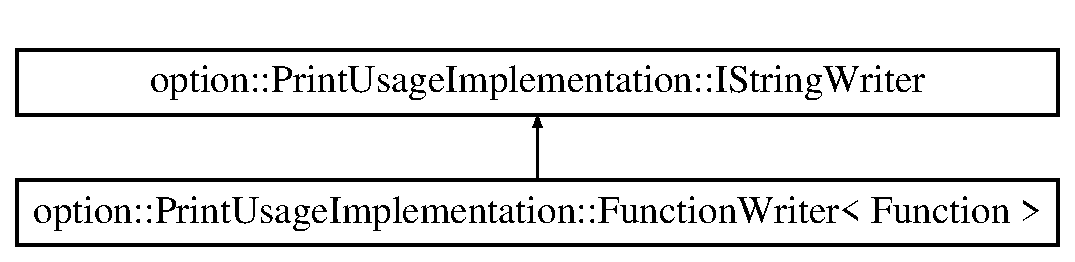
\includegraphics[height=2.000000cm]{structoption_1_1PrintUsageImplementation_1_1FunctionWriter}
\end{center}
\end{figure}
\subsection*{Public Member Functions}
\begin{DoxyCompactItemize}
\item 
\mbox{\Hypertarget{structoption_1_1PrintUsageImplementation_1_1FunctionWriter_aa8e8f237845e210e36ca431d7e503a70}\label{structoption_1_1PrintUsageImplementation_1_1FunctionWriter_aa8e8f237845e210e36ca431d7e503a70}} 
virtual void \hyperlink{structoption_1_1PrintUsageImplementation_1_1FunctionWriter_aa8e8f237845e210e36ca431d7e503a70}{operator()} (const char $\ast$str, int size)
\begin{DoxyCompactList}\small\item\em Writes the given number of chars beginning at the given pointer somewhere. \end{DoxyCompactList}\item 
\mbox{\Hypertarget{structoption_1_1PrintUsageImplementation_1_1FunctionWriter_adc6c3f7ba11b3cad65c018955bab47e5}\label{structoption_1_1PrintUsageImplementation_1_1FunctionWriter_adc6c3f7ba11b3cad65c018955bab47e5}} 
{\bfseries Function\+Writer} (Function $\ast$w)
\end{DoxyCompactItemize}
\subsection*{Public Attributes}
\begin{DoxyCompactItemize}
\item 
\mbox{\Hypertarget{structoption_1_1PrintUsageImplementation_1_1FunctionWriter_a3442e05eb04d2b1ee321193f5b10557b}\label{structoption_1_1PrintUsageImplementation_1_1FunctionWriter_a3442e05eb04d2b1ee321193f5b10557b}} 
Function $\ast$ {\bfseries write}
\end{DoxyCompactItemize}


The documentation for this struct was generated from the following file\+:\begin{DoxyCompactItemize}
\item 
headers/\hyperlink{optionparser_8hpp}{optionparser.\+hpp}\end{DoxyCompactItemize}

\hypertarget{structoption_1_1PrintUsageImplementation_1_1IStringWriter}{}\section{option\+:\+:Print\+Usage\+Implementation\+:\+:I\+String\+Writer Struct Reference}
\label{structoption_1_1PrintUsageImplementation_1_1IStringWriter}\index{option\+::\+Print\+Usage\+Implementation\+::\+I\+String\+Writer@{option\+::\+Print\+Usage\+Implementation\+::\+I\+String\+Writer}}
Inheritance diagram for option\+:\+:Print\+Usage\+Implementation\+:\+:I\+String\+Writer\+:\begin{figure}[H]
\begin{center}
\leavevmode
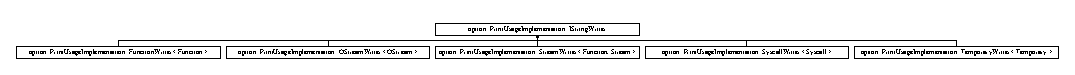
\includegraphics[height=0.555831cm]{structoption_1_1PrintUsageImplementation_1_1IStringWriter}
\end{center}
\end{figure}
\subsection*{Public Member Functions}
\begin{DoxyCompactItemize}
\item 
\mbox{\Hypertarget{structoption_1_1PrintUsageImplementation_1_1IStringWriter_a497172d92e09072a16996c127dd3def8}\label{structoption_1_1PrintUsageImplementation_1_1IStringWriter_a497172d92e09072a16996c127dd3def8}} 
virtual void \hyperlink{structoption_1_1PrintUsageImplementation_1_1IStringWriter_a497172d92e09072a16996c127dd3def8}{operator()} (const char $\ast$, int)
\begin{DoxyCompactList}\small\item\em Writes the given number of chars beginning at the given pointer somewhere. \end{DoxyCompactList}\end{DoxyCompactItemize}


The documentation for this struct was generated from the following file\+:\begin{DoxyCompactItemize}
\item 
headers/\hyperlink{optionparser_8hpp}{optionparser.\+hpp}\end{DoxyCompactItemize}

\hypertarget{classKasiski}{}\section{Kasiski Class Reference}
\label{classKasiski}\index{Kasiski@{Kasiski}}
\subsection*{Public Member Functions}
\begin{DoxyCompactItemize}
\item 
\hyperlink{classKasiski_acdbe405863ad47649cec79084f002206}{Kasiski} (string)
\item 
\mbox{\Hypertarget{classKasiski_a9c17dc2140312977a844de6343fcbe14}\label{classKasiski_a9c17dc2140312977a844de6343fcbe14}} 
set$<$ int $>$ {\bfseries test\+Digraphs} ()
\item 
\mbox{\Hypertarget{classKasiski_a2780b34c1ac811205aaa968f7358cb59}\label{classKasiski_a2780b34c1ac811205aaa968f7358cb59}} 
set$<$ int $>$ {\bfseries test\+Trigraphs} ()
\item 
\mbox{\Hypertarget{classKasiski_ab02b3f86ce0c8b076f222bb0c86d48ad}\label{classKasiski_ab02b3f86ce0c8b076f222bb0c86d48ad}} 
set$<$ int $>$ {\bfseries test\+Crib} ()
\item 
\mbox{\Hypertarget{classKasiski_a10a6c9e944f74c6400738874fa3e0d3b}\label{classKasiski_a10a6c9e944f74c6400738874fa3e0d3b}} 
int {\bfseries guess\+Key\+Using\+Crib} (string)
\item 
set$<$ int $>$ \hyperlink{classKasiski_a82de87eb81569e3d8d595560fa73ee6a}{factors} (int)
\end{DoxyCompactItemize}


\subsection{Constructor \& Destructor Documentation}
\mbox{\Hypertarget{classKasiski_acdbe405863ad47649cec79084f002206}\label{classKasiski_acdbe405863ad47649cec79084f002206}} 
\index{Kasiski@{Kasiski}!Kasiski@{Kasiski}}
\index{Kasiski@{Kasiski}!Kasiski@{Kasiski}}
\subsubsection{\texorpdfstring{Kasiski()}{Kasiski()}}
{\footnotesize\ttfamily Kasiski\+::\+Kasiski (\begin{DoxyParamCaption}\item[{string}]{S }\end{DoxyParamCaption})}

Constructor Not immplemented


\begin{DoxyParams}{Parameters}
{\em file} & Name of file to analyse \\
\hline
\end{DoxyParams}
\begin{DoxyReturn}{Returns}
possible key length as an int 
\end{DoxyReturn}


\subsection{Member Function Documentation}
\mbox{\Hypertarget{classKasiski_a82de87eb81569e3d8d595560fa73ee6a}\label{classKasiski_a82de87eb81569e3d8d595560fa73ee6a}} 
\index{Kasiski@{Kasiski}!factors@{factors}}
\index{factors@{factors}!Kasiski@{Kasiski}}
\subsubsection{\texorpdfstring{factors()}{factors()}}
{\footnotesize\ttfamily set$<$ int $>$ Kasiski\+::factors (\begin{DoxyParamCaption}\item[{int}]{n }\end{DoxyParamCaption})}

Will return the factors of a given integer. Not implemented


\begin{DoxyParams}{Parameters}
{\em n} & integer to break into factors \\
\hline
\end{DoxyParams}
\begin{DoxyReturn}{Returns}
an int set containing factors of n 
\end{DoxyReturn}


The documentation for this class was generated from the following files\+:\begin{DoxyCompactItemize}
\item 
headers/\hyperlink{KeyAnalyser_8hpp}{Key\+Analyser.\+hpp}\item 
sources/\hyperlink{KeyAnalyser_8cpp}{Key\+Analyser.\+cpp}\end{DoxyCompactItemize}

\hypertarget{classKerckhoff}{}\section{Kerckhoff Class Reference}
\label{classKerckhoff}\index{Kerckhoff@{Kerckhoff}}


The documentation for this class was generated from the following file\+:\begin{DoxyCompactItemize}
\item 
headers/\hyperlink{KeyAnalyser_8hpp}{Key\+Analyser.\+hpp}\end{DoxyCompactItemize}

\hypertarget{classKeyBrute}{}\section{Key\+Brute Class Reference}
\label{classKeyBrute}\index{Key\+Brute@{Key\+Brute}}
\subsection*{Public Member Functions}
\begin{DoxyCompactItemize}
\item 
\mbox{\Hypertarget{classKeyBrute_abfeab3a4796354e73b19d1c0064124ac}\label{classKeyBrute_abfeab3a4796354e73b19d1c0064124ac}} 
{\bfseries Key\+Brute} (string, int)
\end{DoxyCompactItemize}


The documentation for this class was generated from the following files\+:\begin{DoxyCompactItemize}
\item 
headers/\hyperlink{KeyAnalyser_8hpp}{Key\+Analyser.\+hpp}\item 
sources/\hyperlink{KeyAnalyser_8cpp}{Key\+Analyser.\+cpp}\end{DoxyCompactItemize}

\hypertarget{classKeyEliminator}{}\section{Key\+Eliminator Class Reference}
\label{classKeyEliminator}\index{Key\+Eliminator@{Key\+Eliminator}}
\subsection*{Public Member Functions}
\begin{DoxyCompactItemize}
\item 
\mbox{\Hypertarget{classKeyEliminator_a19de2303e7fd8d1c1e4f1cddd05abdcb}\label{classKeyEliminator_a19de2303e7fd8d1c1e4f1cddd05abdcb}} 
{\bfseries Key\+Eliminator} (string)
\end{DoxyCompactItemize}


The documentation for this class was generated from the following file\+:\begin{DoxyCompactItemize}
\item 
headers/\hyperlink{KeyAnalyser_8hpp}{Key\+Analyser.\+hpp}\end{DoxyCompactItemize}

\hypertarget{classLanguage}{}\section{Language Class Reference}
\label{classLanguage}\index{Language@{Language}}
Inheritance diagram for Language\+:\begin{figure}[H]
\begin{center}
\leavevmode
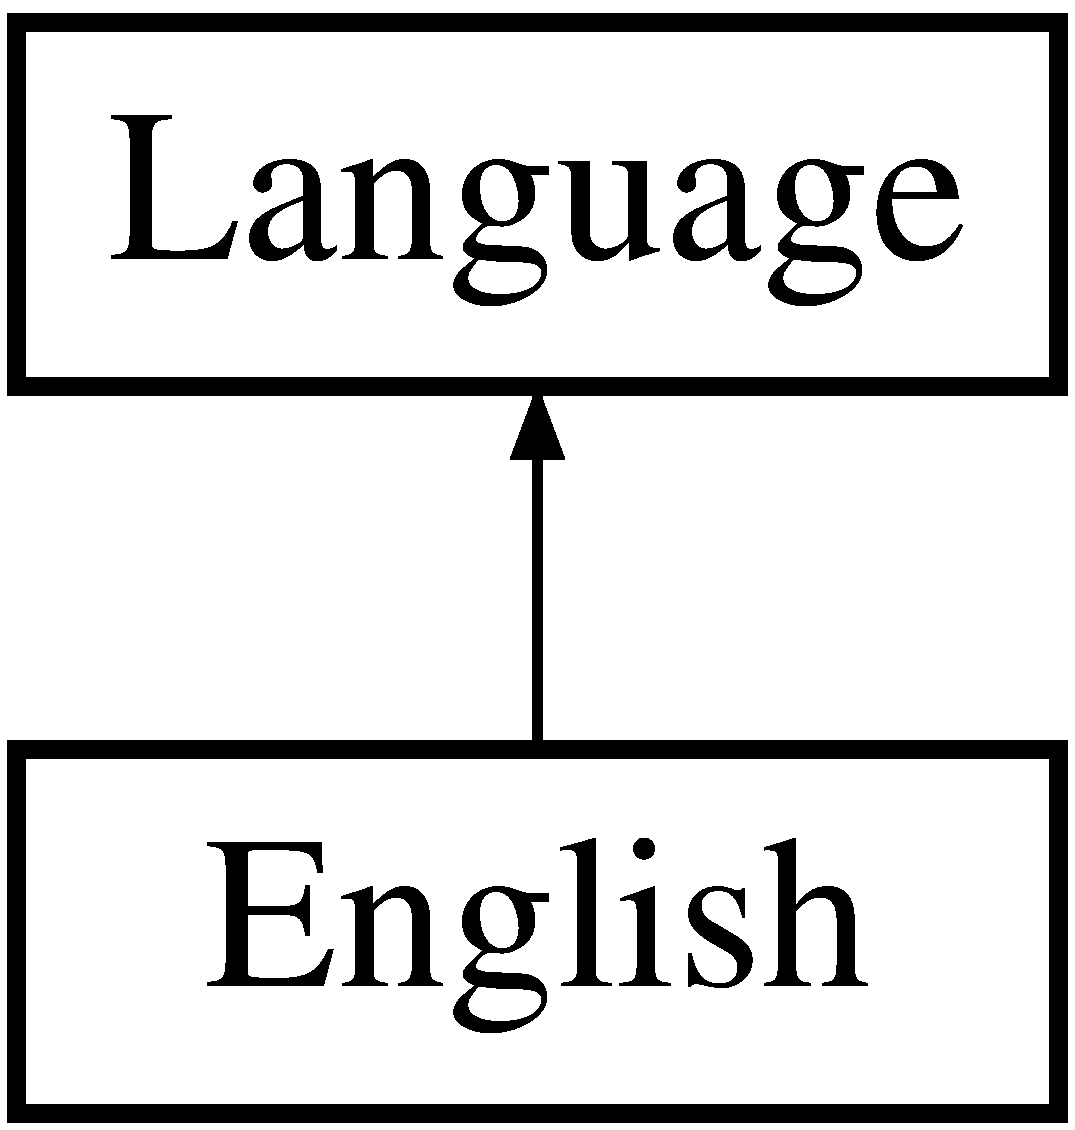
\includegraphics[height=2.000000cm]{classLanguage}
\end{center}
\end{figure}


The documentation for this class was generated from the following file\+:\begin{DoxyCompactItemize}
\item 
headers/\hyperlink{Language_8hpp}{Language.\+hpp}\end{DoxyCompactItemize}

\hypertarget{classoption_1_1PrintUsageImplementation_1_1LinePartIterator}{}\section{option\+:\+:Print\+Usage\+Implementation\+:\+:Line\+Part\+Iterator Class Reference}
\label{classoption_1_1PrintUsageImplementation_1_1LinePartIterator}\index{option\+::\+Print\+Usage\+Implementation\+::\+Line\+Part\+Iterator@{option\+::\+Print\+Usage\+Implementation\+::\+Line\+Part\+Iterator}}
\subsection*{Public Member Functions}
\begin{DoxyCompactItemize}
\item 
\mbox{\Hypertarget{classoption_1_1PrintUsageImplementation_1_1LinePartIterator_a8a61fef9ba907fd4e10ff0fd772ee5e7}\label{classoption_1_1PrintUsageImplementation_1_1LinePartIterator_a8a61fef9ba907fd4e10ff0fd772ee5e7}} 
\hyperlink{classoption_1_1PrintUsageImplementation_1_1LinePartIterator_a8a61fef9ba907fd4e10ff0fd772ee5e7}{Line\+Part\+Iterator} (const \hyperlink{structoption_1_1Descriptor}{Descriptor} usage\mbox{[}$\,$\mbox{]})
\begin{DoxyCompactList}\small\item\em Creates an iterator for {\ttfamily usage}. \end{DoxyCompactList}\item 
bool \hyperlink{classoption_1_1PrintUsageImplementation_1_1LinePartIterator_afe43ca12d399ed3c871e4dc5bf63356e}{next\+Table} ()
\begin{DoxyCompactList}\small\item\em Moves iteration to the next table (if any). Has to be called once on a new \hyperlink{classoption_1_1PrintUsageImplementation_1_1LinePartIterator}{Line\+Part\+Iterator} to move to the 1st table. \end{DoxyCompactList}\item 
\mbox{\Hypertarget{classoption_1_1PrintUsageImplementation_1_1LinePartIterator_a0cbe8ed79ab4958a70b957598dd76fa6}\label{classoption_1_1PrintUsageImplementation_1_1LinePartIterator_a0cbe8ed79ab4958a70b957598dd76fa6}} 
void \hyperlink{classoption_1_1PrintUsageImplementation_1_1LinePartIterator_a0cbe8ed79ab4958a70b957598dd76fa6}{restart\+Table} ()
\begin{DoxyCompactList}\small\item\em Reset iteration to the beginning of the current table. \end{DoxyCompactList}\item 
bool \hyperlink{classoption_1_1PrintUsageImplementation_1_1LinePartIterator_a55d5c3e50f9c1d8cd48f518899a5a48c}{next\+Row} ()
\begin{DoxyCompactList}\small\item\em Moves iteration to the next row (if any). Has to be called once after each call to \hyperlink{classoption_1_1PrintUsageImplementation_1_1LinePartIterator_afe43ca12d399ed3c871e4dc5bf63356e}{next\+Table()} to move to the 1st row of the table. \end{DoxyCompactList}\item 
\mbox{\Hypertarget{classoption_1_1PrintUsageImplementation_1_1LinePartIterator_a96c448939f33a811174ea7b5addb312e}\label{classoption_1_1PrintUsageImplementation_1_1LinePartIterator_a96c448939f33a811174ea7b5addb312e}} 
void \hyperlink{classoption_1_1PrintUsageImplementation_1_1LinePartIterator_a96c448939f33a811174ea7b5addb312e}{restart\+Row} ()
\begin{DoxyCompactList}\small\item\em Reset iteration to the beginning of the current row. \end{DoxyCompactList}\item 
bool \hyperlink{classoption_1_1PrintUsageImplementation_1_1LinePartIterator_a58b8743da57de2d108472eee60324df6}{next} ()
\begin{DoxyCompactList}\small\item\em Moves iteration to the next part (if any). Has to be called once after each call to \hyperlink{classoption_1_1PrintUsageImplementation_1_1LinePartIterator_a55d5c3e50f9c1d8cd48f518899a5a48c}{next\+Row()} to move to the 1st part of the row. \end{DoxyCompactList}\item 
\mbox{\Hypertarget{classoption_1_1PrintUsageImplementation_1_1LinePartIterator_afa41382acabcd37ca70f7e8b9994b8c0}\label{classoption_1_1PrintUsageImplementation_1_1LinePartIterator_afa41382acabcd37ca70f7e8b9994b8c0}} 
int \hyperlink{classoption_1_1PrintUsageImplementation_1_1LinePartIterator_afa41382acabcd37ca70f7e8b9994b8c0}{column} ()
\begin{DoxyCompactList}\small\item\em Returns the index (counting from 0) of the column in which the part pointed to by \hyperlink{classoption_1_1PrintUsageImplementation_1_1LinePartIterator_ada26229add63bd479c7877f2f8e32908}{data()} is located. \end{DoxyCompactList}\item 
\mbox{\Hypertarget{classoption_1_1PrintUsageImplementation_1_1LinePartIterator_a8ad1201d95bf0bd9453a731da8c15a10}\label{classoption_1_1PrintUsageImplementation_1_1LinePartIterator_a8ad1201d95bf0bd9453a731da8c15a10}} 
int \hyperlink{classoption_1_1PrintUsageImplementation_1_1LinePartIterator_a8ad1201d95bf0bd9453a731da8c15a10}{line} ()
\begin{DoxyCompactList}\small\item\em Returns the index (counting from 0) of the line within the current column this part belongs to. \end{DoxyCompactList}\item 
\mbox{\Hypertarget{classoption_1_1PrintUsageImplementation_1_1LinePartIterator_a557e521cb41e951a34df2737d25f9dce}\label{classoption_1_1PrintUsageImplementation_1_1LinePartIterator_a557e521cb41e951a34df2737d25f9dce}} 
int \hyperlink{classoption_1_1PrintUsageImplementation_1_1LinePartIterator_a557e521cb41e951a34df2737d25f9dce}{length} ()
\begin{DoxyCompactList}\small\item\em Returns the length of the part pointed to by \hyperlink{classoption_1_1PrintUsageImplementation_1_1LinePartIterator_ada26229add63bd479c7877f2f8e32908}{data()} in raw chars (not U\+T\+F-\/8 characters). \end{DoxyCompactList}\item 
\mbox{\Hypertarget{classoption_1_1PrintUsageImplementation_1_1LinePartIterator_a03b6fedfe805d7fc73216da5cd33270e}\label{classoption_1_1PrintUsageImplementation_1_1LinePartIterator_a03b6fedfe805d7fc73216da5cd33270e}} 
int \hyperlink{classoption_1_1PrintUsageImplementation_1_1LinePartIterator_a03b6fedfe805d7fc73216da5cd33270e}{screen\+Length} ()
\begin{DoxyCompactList}\small\item\em Returns the width in screen columns of the part pointed to by \hyperlink{classoption_1_1PrintUsageImplementation_1_1LinePartIterator_ada26229add63bd479c7877f2f8e32908}{data()}. Takes multi-\/byte U\+T\+F-\/8 sequences and wide characters into account. \end{DoxyCompactList}\item 
\mbox{\Hypertarget{classoption_1_1PrintUsageImplementation_1_1LinePartIterator_ada26229add63bd479c7877f2f8e32908}\label{classoption_1_1PrintUsageImplementation_1_1LinePartIterator_ada26229add63bd479c7877f2f8e32908}} 
const char $\ast$ \hyperlink{classoption_1_1PrintUsageImplementation_1_1LinePartIterator_ada26229add63bd479c7877f2f8e32908}{data} ()
\begin{DoxyCompactList}\small\item\em Returns the current part of the iteration. \end{DoxyCompactList}\end{DoxyCompactItemize}


\subsection{Member Function Documentation}
\mbox{\Hypertarget{classoption_1_1PrintUsageImplementation_1_1LinePartIterator_a58b8743da57de2d108472eee60324df6}\label{classoption_1_1PrintUsageImplementation_1_1LinePartIterator_a58b8743da57de2d108472eee60324df6}} 
\index{option\+::\+Print\+Usage\+Implementation\+::\+Line\+Part\+Iterator@{option\+::\+Print\+Usage\+Implementation\+::\+Line\+Part\+Iterator}!next@{next}}
\index{next@{next}!option\+::\+Print\+Usage\+Implementation\+::\+Line\+Part\+Iterator@{option\+::\+Print\+Usage\+Implementation\+::\+Line\+Part\+Iterator}}
\subsubsection{\texorpdfstring{next()}{next()}}
{\footnotesize\ttfamily bool option\+::\+Print\+Usage\+Implementation\+::\+Line\+Part\+Iterator\+::next (\begin{DoxyParamCaption}{ }\end{DoxyParamCaption})\hspace{0.3cm}{\ttfamily [inline]}}



Moves iteration to the next part (if any). Has to be called once after each call to \hyperlink{classoption_1_1PrintUsageImplementation_1_1LinePartIterator_a55d5c3e50f9c1d8cd48f518899a5a48c}{next\+Row()} to move to the 1st part of the row. 


\begin{DoxyRetVals}{Return values}
{\em false} & if moving to next part failed because no further part exists.\\
\hline
\end{DoxyRetVals}
See \hyperlink{classoption_1_1PrintUsageImplementation_1_1LinePartIterator}{Line\+Part\+Iterator} for details about the iteration. \mbox{\Hypertarget{classoption_1_1PrintUsageImplementation_1_1LinePartIterator_a55d5c3e50f9c1d8cd48f518899a5a48c}\label{classoption_1_1PrintUsageImplementation_1_1LinePartIterator_a55d5c3e50f9c1d8cd48f518899a5a48c}} 
\index{option\+::\+Print\+Usage\+Implementation\+::\+Line\+Part\+Iterator@{option\+::\+Print\+Usage\+Implementation\+::\+Line\+Part\+Iterator}!next\+Row@{next\+Row}}
\index{next\+Row@{next\+Row}!option\+::\+Print\+Usage\+Implementation\+::\+Line\+Part\+Iterator@{option\+::\+Print\+Usage\+Implementation\+::\+Line\+Part\+Iterator}}
\subsubsection{\texorpdfstring{next\+Row()}{nextRow()}}
{\footnotesize\ttfamily bool option\+::\+Print\+Usage\+Implementation\+::\+Line\+Part\+Iterator\+::next\+Row (\begin{DoxyParamCaption}{ }\end{DoxyParamCaption})\hspace{0.3cm}{\ttfamily [inline]}}



Moves iteration to the next row (if any). Has to be called once after each call to \hyperlink{classoption_1_1PrintUsageImplementation_1_1LinePartIterator_afe43ca12d399ed3c871e4dc5bf63356e}{next\+Table()} to move to the 1st row of the table. 


\begin{DoxyRetVals}{Return values}
{\em false} & if moving to next row failed because no further row exists. \\
\hline
\end{DoxyRetVals}
\mbox{\Hypertarget{classoption_1_1PrintUsageImplementation_1_1LinePartIterator_afe43ca12d399ed3c871e4dc5bf63356e}\label{classoption_1_1PrintUsageImplementation_1_1LinePartIterator_afe43ca12d399ed3c871e4dc5bf63356e}} 
\index{option\+::\+Print\+Usage\+Implementation\+::\+Line\+Part\+Iterator@{option\+::\+Print\+Usage\+Implementation\+::\+Line\+Part\+Iterator}!next\+Table@{next\+Table}}
\index{next\+Table@{next\+Table}!option\+::\+Print\+Usage\+Implementation\+::\+Line\+Part\+Iterator@{option\+::\+Print\+Usage\+Implementation\+::\+Line\+Part\+Iterator}}
\subsubsection{\texorpdfstring{next\+Table()}{nextTable()}}
{\footnotesize\ttfamily bool option\+::\+Print\+Usage\+Implementation\+::\+Line\+Part\+Iterator\+::next\+Table (\begin{DoxyParamCaption}{ }\end{DoxyParamCaption})\hspace{0.3cm}{\ttfamily [inline]}}



Moves iteration to the next table (if any). Has to be called once on a new \hyperlink{classoption_1_1PrintUsageImplementation_1_1LinePartIterator}{Line\+Part\+Iterator} to move to the 1st table. 


\begin{DoxyRetVals}{Return values}
{\em false} & if moving to next table failed because no further table exists. \\
\hline
\end{DoxyRetVals}


The documentation for this class was generated from the following file\+:\begin{DoxyCompactItemize}
\item 
headers/\hyperlink{optionparser_8hpp}{optionparser.\+hpp}\end{DoxyCompactItemize}

\hypertarget{classoption_1_1PrintUsageImplementation_1_1LineWrapper}{}\section{option\+:\+:Print\+Usage\+Implementation\+:\+:Line\+Wrapper Class Reference}
\label{classoption_1_1PrintUsageImplementation_1_1LineWrapper}\index{option\+::\+Print\+Usage\+Implementation\+::\+Line\+Wrapper@{option\+::\+Print\+Usage\+Implementation\+::\+Line\+Wrapper}}
\subsection*{Public Member Functions}
\begin{DoxyCompactItemize}
\item 
\mbox{\Hypertarget{classoption_1_1PrintUsageImplementation_1_1LineWrapper_a9383db9fd3fb18ce091db63ce0b149fd}\label{classoption_1_1PrintUsageImplementation_1_1LineWrapper_a9383db9fd3fb18ce091db63ce0b149fd}} 
void \hyperlink{classoption_1_1PrintUsageImplementation_1_1LineWrapper_a9383db9fd3fb18ce091db63ce0b149fd}{flush} (\hyperlink{structoption_1_1PrintUsageImplementation_1_1IStringWriter}{I\+String\+Writer} \&write)
\begin{DoxyCompactList}\small\item\em Writes out all remaining data from the \hyperlink{classoption_1_1PrintUsageImplementation_1_1LineWrapper}{Line\+Wrapper} using {\ttfamily write}. Unlike \hyperlink{classoption_1_1PrintUsageImplementation_1_1LineWrapper_add20eca40865ad892d6c28b412ac14d5}{process()} this method indents all lines including the first and will output a \textbackslash{}n at the end (but only if something has been written). \end{DoxyCompactList}\item 
void \hyperlink{classoption_1_1PrintUsageImplementation_1_1LineWrapper_add20eca40865ad892d6c28b412ac14d5}{process} (\hyperlink{structoption_1_1PrintUsageImplementation_1_1IStringWriter}{I\+String\+Writer} \&write, const char $\ast$data, int len)
\begin{DoxyCompactList}\small\item\em Process, wrap and output the next piece of data. \end{DoxyCompactList}\item 
\hyperlink{classoption_1_1PrintUsageImplementation_1_1LineWrapper_a288f16b6e928e9f54f48e13ff6817e95}{Line\+Wrapper} (int x1, int x2)
\begin{DoxyCompactList}\small\item\em Constructs a \hyperlink{classoption_1_1PrintUsageImplementation_1_1LineWrapper}{Line\+Wrapper} that wraps its output to fit into screen columns {\ttfamily x1} (incl.) to {\ttfamily x2} (excl.). \end{DoxyCompactList}\end{DoxyCompactItemize}


\subsection{Constructor \& Destructor Documentation}
\mbox{\Hypertarget{classoption_1_1PrintUsageImplementation_1_1LineWrapper_a288f16b6e928e9f54f48e13ff6817e95}\label{classoption_1_1PrintUsageImplementation_1_1LineWrapper_a288f16b6e928e9f54f48e13ff6817e95}} 
\index{option\+::\+Print\+Usage\+Implementation\+::\+Line\+Wrapper@{option\+::\+Print\+Usage\+Implementation\+::\+Line\+Wrapper}!Line\+Wrapper@{Line\+Wrapper}}
\index{Line\+Wrapper@{Line\+Wrapper}!option\+::\+Print\+Usage\+Implementation\+::\+Line\+Wrapper@{option\+::\+Print\+Usage\+Implementation\+::\+Line\+Wrapper}}
\subsubsection{\texorpdfstring{Line\+Wrapper()}{LineWrapper()}}
{\footnotesize\ttfamily option\+::\+Print\+Usage\+Implementation\+::\+Line\+Wrapper\+::\+Line\+Wrapper (\begin{DoxyParamCaption}\item[{int}]{x1,  }\item[{int}]{x2 }\end{DoxyParamCaption})\hspace{0.3cm}{\ttfamily [inline]}}



Constructs a \hyperlink{classoption_1_1PrintUsageImplementation_1_1LineWrapper}{Line\+Wrapper} that wraps its output to fit into screen columns {\ttfamily x1} (incl.) to {\ttfamily x2} (excl.). 

{\ttfamily x1} gives the indentation \hyperlink{classoption_1_1PrintUsageImplementation_1_1LineWrapper}{Line\+Wrapper} uses if it needs to indent. 

\subsection{Member Function Documentation}
\mbox{\Hypertarget{classoption_1_1PrintUsageImplementation_1_1LineWrapper_add20eca40865ad892d6c28b412ac14d5}\label{classoption_1_1PrintUsageImplementation_1_1LineWrapper_add20eca40865ad892d6c28b412ac14d5}} 
\index{option\+::\+Print\+Usage\+Implementation\+::\+Line\+Wrapper@{option\+::\+Print\+Usage\+Implementation\+::\+Line\+Wrapper}!process@{process}}
\index{process@{process}!option\+::\+Print\+Usage\+Implementation\+::\+Line\+Wrapper@{option\+::\+Print\+Usage\+Implementation\+::\+Line\+Wrapper}}
\subsubsection{\texorpdfstring{process()}{process()}}
{\footnotesize\ttfamily void option\+::\+Print\+Usage\+Implementation\+::\+Line\+Wrapper\+::process (\begin{DoxyParamCaption}\item[{\hyperlink{structoption_1_1PrintUsageImplementation_1_1IStringWriter}{I\+String\+Writer} \&}]{write,  }\item[{const char $\ast$}]{data,  }\item[{int}]{len }\end{DoxyParamCaption})\hspace{0.3cm}{\ttfamily [inline]}}



Process, wrap and output the next piece of data. 

\hyperlink{classoption_1_1PrintUsageImplementation_1_1LineWrapper_add20eca40865ad892d6c28b412ac14d5}{process()} will output at least one line of output. This is not necessarily the {\ttfamily data} passed in. It may be data queued from a prior call to \hyperlink{classoption_1_1PrintUsageImplementation_1_1LineWrapper_add20eca40865ad892d6c28b412ac14d5}{process()}. If the internal buffer is full, more than 1 line will be output.

\hyperlink{classoption_1_1PrintUsageImplementation_1_1LineWrapper_add20eca40865ad892d6c28b412ac14d5}{process()} assumes that the a proper amount of indentation has already been output. It won\textquotesingle{}t write any further indentation before the 1st line. If more than 1 line is written due to buffer constraints, the lines following the first will be indented by this method, though.

No \textbackslash{}n is written by this method after the last line that is written.


\begin{DoxyParams}{Parameters}
{\em write} & where to write the data. \\
\hline
{\em data} & the new chunk of data to write. \\
\hline
{\em len} & the length of the chunk of data to write. \\
\hline
\end{DoxyParams}


The documentation for this class was generated from the following file\+:\begin{DoxyCompactItemize}
\item 
headers/\hyperlink{optionparser_8hpp}{optionparser.\+hpp}\end{DoxyCompactItemize}

\hypertarget{classoption_1_1Option}{}\section{option\+:\+:Option Class Reference}
\label{classoption_1_1Option}\index{option\+::\+Option@{option\+::\+Option}}


A parsed option from the command line together with its argument if it has one.  




{\ttfamily \#include $<$optionparser.\+hpp$>$}

\subsection*{Public Member Functions}
\begin{DoxyCompactItemize}
\item 
int \hyperlink{classoption_1_1Option_a5268a69e1a91137186ab772574296da0}{type} () const
\begin{DoxyCompactList}\small\item\em Returns \hyperlink{structoption_1_1Descriptor_a1b220dabd8aad075fa441a80f9b9343c}{Descriptor\+::type} of this \hyperlink{classoption_1_1Option}{Option}\textquotesingle{}s \hyperlink{structoption_1_1Descriptor}{Descriptor}, or 0 if this \hyperlink{classoption_1_1Option}{Option} is invalid (unused). \end{DoxyCompactList}\item 
\mbox{\Hypertarget{classoption_1_1Option_a847d12e8e76add769fbd01c703e48682}\label{classoption_1_1Option_a847d12e8e76add769fbd01c703e48682}} 
int \hyperlink{classoption_1_1Option_a847d12e8e76add769fbd01c703e48682}{index} () const
\begin{DoxyCompactList}\small\item\em Returns \hyperlink{structoption_1_1Descriptor_a1fee8ac44f529c99ac2b1149b4c391b1}{Descriptor\+::index} of this \hyperlink{classoption_1_1Option}{Option}\textquotesingle{}s \hyperlink{structoption_1_1Descriptor}{Descriptor}, or -\/1 if this \hyperlink{classoption_1_1Option}{Option} is invalid (unused). \end{DoxyCompactList}\item 
int \hyperlink{classoption_1_1Option_a8a632dcd89af60fe0806deb756c08f14}{count} ()
\begin{DoxyCompactList}\small\item\em Returns the number of times this \hyperlink{classoption_1_1Option}{Option} (or others with the same \hyperlink{structoption_1_1Descriptor_a1fee8ac44f529c99ac2b1149b4c391b1}{Descriptor\+::index}) occurs in the argument vector. \end{DoxyCompactList}\item 
bool \hyperlink{classoption_1_1Option_af51f53a553ef46110e36008a58466a2e}{is\+First} () const
\begin{DoxyCompactList}\small\item\em Returns true iff this is the first element of the linked list. \end{DoxyCompactList}\item 
bool \hyperlink{classoption_1_1Option_a36fa8fde6fce89462ded79ab56180ff7}{is\+Last} () const
\begin{DoxyCompactList}\small\item\em Returns true iff this is the last element of the linked list. \end{DoxyCompactList}\item 
\hyperlink{classoption_1_1Option}{Option} $\ast$ \hyperlink{classoption_1_1Option_abb4e13cd7c90999c8a6b1f871cece283}{first} ()
\begin{DoxyCompactList}\small\item\em Returns a pointer to the first element of the linked list. \end{DoxyCompactList}\item 
\hyperlink{classoption_1_1Option}{Option} $\ast$ \hyperlink{classoption_1_1Option_afe2aff68191e55b59c53fac3dbbcd7c3}{last} ()
\begin{DoxyCompactList}\small\item\em Returns a pointer to the last element of the linked list. \end{DoxyCompactList}\item 
\hyperlink{classoption_1_1Option}{Option} $\ast$ \hyperlink{classoption_1_1Option_a4d12001a91b0b35cf47437d0c60d2b52}{prev} ()
\begin{DoxyCompactList}\small\item\em Returns a pointer to the previous element of the linked list or N\+U\+LL if called on \hyperlink{classoption_1_1Option_abb4e13cd7c90999c8a6b1f871cece283}{first()}. \end{DoxyCompactList}\item 
\hyperlink{classoption_1_1Option}{Option} $\ast$ \hyperlink{classoption_1_1Option_a1226e45dc2de30f269b2aff1784bbee7}{prevwrap} ()
\begin{DoxyCompactList}\small\item\em Returns a pointer to the previous element of the linked list with wrap-\/around from \hyperlink{classoption_1_1Option_abb4e13cd7c90999c8a6b1f871cece283}{first()} to \hyperlink{classoption_1_1Option_afe2aff68191e55b59c53fac3dbbcd7c3}{last()}. \end{DoxyCompactList}\item 
\hyperlink{classoption_1_1Option}{Option} $\ast$ \hyperlink{classoption_1_1Option_a59ae9aed505f4d410633bb36478a32be}{next} ()
\begin{DoxyCompactList}\small\item\em Returns a pointer to the next element of the linked list or N\+U\+LL if called on \hyperlink{classoption_1_1Option_afe2aff68191e55b59c53fac3dbbcd7c3}{last()}. \end{DoxyCompactList}\item 
\hyperlink{classoption_1_1Option}{Option} $\ast$ \hyperlink{classoption_1_1Option_ae8d8c058af3c781cb1d444998df48fef}{nextwrap} ()
\begin{DoxyCompactList}\small\item\em Returns a pointer to the next element of the linked list with wrap-\/around from \hyperlink{classoption_1_1Option_afe2aff68191e55b59c53fac3dbbcd7c3}{last()} to \hyperlink{classoption_1_1Option_abb4e13cd7c90999c8a6b1f871cece283}{first()}. \end{DoxyCompactList}\item 
void \hyperlink{classoption_1_1Option_a59030822a1ec4e667e6c288d7e5ec961}{append} (\hyperlink{classoption_1_1Option}{Option} $\ast$new\+\_\+last)
\begin{DoxyCompactList}\small\item\em Makes {\ttfamily new\+\_\+last} the new \hyperlink{classoption_1_1Option_afe2aff68191e55b59c53fac3dbbcd7c3}{last()} by chaining it into the list after \hyperlink{classoption_1_1Option_afe2aff68191e55b59c53fac3dbbcd7c3}{last()}. \end{DoxyCompactList}\item 
\hyperlink{classoption_1_1Option_a3c0504baaa809c622d59c2c09f83e25b}{operator const Option $\ast$} () const
\begin{DoxyCompactList}\small\item\em Casts from \hyperlink{classoption_1_1Option}{Option} to const Option$\ast$ but only if this \hyperlink{classoption_1_1Option}{Option} is valid. \end{DoxyCompactList}\item 
\hyperlink{classoption_1_1Option_ac5b9235d79208035d97e41fe17ba04d6}{operator Option $\ast$} ()
\begin{DoxyCompactList}\small\item\em Casts from \hyperlink{classoption_1_1Option}{Option} to Option$\ast$ but only if this \hyperlink{classoption_1_1Option}{Option} is valid. \end{DoxyCompactList}\item 
\mbox{\Hypertarget{classoption_1_1Option_aa2810152fc23b14175b115d1a7d38095}\label{classoption_1_1Option_aa2810152fc23b14175b115d1a7d38095}} 
\hyperlink{classoption_1_1Option_aa2810152fc23b14175b115d1a7d38095}{Option} ()
\begin{DoxyCompactList}\small\item\em Creates a new \hyperlink{classoption_1_1Option}{Option} that is a one-\/element linked list and has N\+U\+LL \hyperlink{classoption_1_1Option_af8d664a7b5de1425008b1812a90a0c23}{desc}, \hyperlink{classoption_1_1Option_a02a76b4896abd22d0ba8514362261de9}{name}, \hyperlink{classoption_1_1Option_a402be734987458364b0f473acae36238}{arg} and \hyperlink{classoption_1_1Option_a3aa2957b19ad5815873441b415d56050}{namelen}. \end{DoxyCompactList}\item 
\hyperlink{classoption_1_1Option_a385221e2a8f37c548f0d5777bfddb216}{Option} (const \hyperlink{structoption_1_1Descriptor}{Descriptor} $\ast$desc\+\_\+, const char $\ast$name\+\_\+, const char $\ast$arg\+\_\+)
\begin{DoxyCompactList}\small\item\em Creates a new \hyperlink{classoption_1_1Option}{Option} that is a one-\/element linked list and has the given values for \hyperlink{classoption_1_1Option_af8d664a7b5de1425008b1812a90a0c23}{desc}, \hyperlink{classoption_1_1Option_a02a76b4896abd22d0ba8514362261de9}{name} and \hyperlink{classoption_1_1Option_a402be734987458364b0f473acae36238}{arg}. \end{DoxyCompactList}\item 
void \hyperlink{classoption_1_1Option_adb4b44f3778df8f28a04c48bd1b4a72b}{operator=} (const \hyperlink{classoption_1_1Option}{Option} \&orig)
\begin{DoxyCompactList}\small\item\em Makes {\ttfamily $\ast$this} a copy of {\ttfamily orig} except for the linked list pointers. \end{DoxyCompactList}\item 
\hyperlink{classoption_1_1Option_a4053240fecad1a3b1d8e4dc06b7aa8c4}{Option} (const \hyperlink{classoption_1_1Option}{Option} \&orig)
\begin{DoxyCompactList}\small\item\em Makes {\ttfamily $\ast$this} a copy of {\ttfamily orig} except for the linked list pointers. \end{DoxyCompactList}\end{DoxyCompactItemize}
\subsection*{Public Attributes}
\begin{DoxyCompactItemize}
\item 
const \hyperlink{structoption_1_1Descriptor}{Descriptor} $\ast$ \hyperlink{classoption_1_1Option_af8d664a7b5de1425008b1812a90a0c23}{desc}
\begin{DoxyCompactList}\small\item\em Pointer to this \hyperlink{classoption_1_1Option}{Option}\textquotesingle{}s \hyperlink{structoption_1_1Descriptor}{Descriptor}. \end{DoxyCompactList}\item 
const char $\ast$ \hyperlink{classoption_1_1Option_a02a76b4896abd22d0ba8514362261de9}{name}
\begin{DoxyCompactList}\small\item\em The name of the option as used on the command line. \end{DoxyCompactList}\item 
const char $\ast$ \hyperlink{classoption_1_1Option_a402be734987458364b0f473acae36238}{arg}
\begin{DoxyCompactList}\small\item\em Pointer to this \hyperlink{classoption_1_1Option}{Option}\textquotesingle{}s argument (if any). \end{DoxyCompactList}\item 
int \hyperlink{classoption_1_1Option_a3aa2957b19ad5815873441b415d56050}{namelen}
\begin{DoxyCompactList}\small\item\em The length of the option \hyperlink{classoption_1_1Option_a02a76b4896abd22d0ba8514362261de9}{name}. \end{DoxyCompactList}\end{DoxyCompactItemize}


\subsection{Detailed Description}
A parsed option from the command line together with its argument if it has one. 

The \hyperlink{classoption_1_1Parser}{Parser} chains all parsed options with the same \hyperlink{structoption_1_1Descriptor_a1fee8ac44f529c99ac2b1149b4c391b1}{Descriptor\+::index} together to form a linked list. This allows you to easily implement all of the common ways of handling repeated options and enable/disable pairs.

\begin{DoxyItemize}
\item Test for presence of a switch in the argument vector\+: 
\begin{DoxyCode}
\textcolor{keywordflow}{if} ( options[QUIET] ) ... 
\end{DoxyCode}
 \item Evaluate --enable-\/foo/--disable-\/foo pair where the last one used wins\+: 
\begin{DoxyCode}
\textcolor{keywordflow}{if} ( options[FOO].\hyperlink{classoption_1_1Option_afe2aff68191e55b59c53fac3dbbcd7c3}{last}()->\hyperlink{classoption_1_1Option_a5268a69e1a91137186ab772574296da0}{type}() == DISABLE ) ... 
\end{DoxyCode}
 \item Cumulative option (-\/v verbose, -\/vv more verbose, -\/vvv even more verbose)\+: 
\begin{DoxyCode}
\textcolor{keywordtype}{int} verbosity = options[VERBOSE].count(); 
\end{DoxyCode}
 \item Iterate over all --file=$<$fname$>$ arguments\+: 
\begin{DoxyCode}
\textcolor{keywordflow}{for} (\hyperlink{classoption_1_1Option_aa2810152fc23b14175b115d1a7d38095}{Option}* opt = options[FILE]; opt; opt = opt->next())
 fname = opt->arg; ... 
\end{DoxyCode}
 \end{DoxyItemize}


\subsection{Constructor \& Destructor Documentation}
\mbox{\Hypertarget{classoption_1_1Option_a385221e2a8f37c548f0d5777bfddb216}\label{classoption_1_1Option_a385221e2a8f37c548f0d5777bfddb216}} 
\index{option\+::\+Option@{option\+::\+Option}!Option@{Option}}
\index{Option@{Option}!option\+::\+Option@{option\+::\+Option}}
\subsubsection{\texorpdfstring{Option()}{Option()}\hspace{0.1cm}{\footnotesize\ttfamily [1/2]}}
{\footnotesize\ttfamily option\+::\+Option\+::\+Option (\begin{DoxyParamCaption}\item[{const \hyperlink{structoption_1_1Descriptor}{Descriptor} $\ast$}]{desc\+\_\+,  }\item[{const char $\ast$}]{name\+\_\+,  }\item[{const char $\ast$}]{arg\+\_\+ }\end{DoxyParamCaption})\hspace{0.3cm}{\ttfamily [inline]}}



Creates a new \hyperlink{classoption_1_1Option}{Option} that is a one-\/element linked list and has the given values for \hyperlink{classoption_1_1Option_af8d664a7b5de1425008b1812a90a0c23}{desc}, \hyperlink{classoption_1_1Option_a02a76b4896abd22d0ba8514362261de9}{name} and \hyperlink{classoption_1_1Option_a402be734987458364b0f473acae36238}{arg}. 

If {\ttfamily name\+\_\+} points at a character other than \textquotesingle{}-\/\textquotesingle{} it will be assumed to refer to a short option and \hyperlink{classoption_1_1Option_a3aa2957b19ad5815873441b415d56050}{namelen} will be set to 1. Otherwise the length will extend to the first \textquotesingle{}=\textquotesingle{} character or the string\textquotesingle{}s 0-\/terminator. \mbox{\Hypertarget{classoption_1_1Option_a4053240fecad1a3b1d8e4dc06b7aa8c4}\label{classoption_1_1Option_a4053240fecad1a3b1d8e4dc06b7aa8c4}} 
\index{option\+::\+Option@{option\+::\+Option}!Option@{Option}}
\index{Option@{Option}!option\+::\+Option@{option\+::\+Option}}
\subsubsection{\texorpdfstring{Option()}{Option()}\hspace{0.1cm}{\footnotesize\ttfamily [2/2]}}
{\footnotesize\ttfamily option\+::\+Option\+::\+Option (\begin{DoxyParamCaption}\item[{const \hyperlink{classoption_1_1Option}{Option} \&}]{orig }\end{DoxyParamCaption})\hspace{0.3cm}{\ttfamily [inline]}}



Makes {\ttfamily $\ast$this} a copy of {\ttfamily orig} except for the linked list pointers. 

After this operation {\ttfamily $\ast$this} will be a one-\/element linked list. 

\subsection{Member Function Documentation}
\mbox{\Hypertarget{classoption_1_1Option_a59030822a1ec4e667e6c288d7e5ec961}\label{classoption_1_1Option_a59030822a1ec4e667e6c288d7e5ec961}} 
\index{option\+::\+Option@{option\+::\+Option}!append@{append}}
\index{append@{append}!option\+::\+Option@{option\+::\+Option}}
\subsubsection{\texorpdfstring{append()}{append()}}
{\footnotesize\ttfamily void option\+::\+Option\+::append (\begin{DoxyParamCaption}\item[{\hyperlink{classoption_1_1Option}{Option} $\ast$}]{new\+\_\+last }\end{DoxyParamCaption})\hspace{0.3cm}{\ttfamily [inline]}}



Makes {\ttfamily new\+\_\+last} the new \hyperlink{classoption_1_1Option_afe2aff68191e55b59c53fac3dbbcd7c3}{last()} by chaining it into the list after \hyperlink{classoption_1_1Option_afe2aff68191e55b59c53fac3dbbcd7c3}{last()}. 

It doesn\textquotesingle{}t matter which element you call \hyperlink{classoption_1_1Option_a59030822a1ec4e667e6c288d7e5ec961}{append()} on. The new element will always be appended to \hyperlink{classoption_1_1Option_afe2aff68191e55b59c53fac3dbbcd7c3}{last()}.

\begin{DoxyAttention}{Attention}
{\ttfamily new\+\_\+last} must not yet be part of a list, or that list will become corrupted, because this method does not unchain {\ttfamily new\+\_\+last} from an existing list. 
\end{DoxyAttention}
\mbox{\Hypertarget{classoption_1_1Option_a8a632dcd89af60fe0806deb756c08f14}\label{classoption_1_1Option_a8a632dcd89af60fe0806deb756c08f14}} 
\index{option\+::\+Option@{option\+::\+Option}!count@{count}}
\index{count@{count}!option\+::\+Option@{option\+::\+Option}}
\subsubsection{\texorpdfstring{count()}{count()}}
{\footnotesize\ttfamily int option\+::\+Option\+::count (\begin{DoxyParamCaption}{ }\end{DoxyParamCaption})\hspace{0.3cm}{\ttfamily [inline]}}



Returns the number of times this \hyperlink{classoption_1_1Option}{Option} (or others with the same \hyperlink{structoption_1_1Descriptor_a1fee8ac44f529c99ac2b1149b4c391b1}{Descriptor\+::index}) occurs in the argument vector. 

This corresponds to the number of elements in the linked list this \hyperlink{classoption_1_1Option}{Option} is part of. It doesn\textquotesingle{}t matter on which element you call \hyperlink{classoption_1_1Option_a8a632dcd89af60fe0806deb756c08f14}{count()}. The return value is always the same.

Use this to implement cumulative options, such as -\/v, -\/vv, -\/vvv for different verbosity levels.

Returns 0 when called for an unused/invalid option. \mbox{\Hypertarget{classoption_1_1Option_abb4e13cd7c90999c8a6b1f871cece283}\label{classoption_1_1Option_abb4e13cd7c90999c8a6b1f871cece283}} 
\index{option\+::\+Option@{option\+::\+Option}!first@{first}}
\index{first@{first}!option\+::\+Option@{option\+::\+Option}}
\subsubsection{\texorpdfstring{first()}{first()}}
{\footnotesize\ttfamily \hyperlink{classoption_1_1Option}{Option}$\ast$ option\+::\+Option\+::first (\begin{DoxyParamCaption}{ }\end{DoxyParamCaption})\hspace{0.3cm}{\ttfamily [inline]}}



Returns a pointer to the first element of the linked list. 

Use this when you want the first occurrence of an option on the command line to take precedence. Note that this is not the way most programs handle options. You should probably be using \hyperlink{classoption_1_1Option_afe2aff68191e55b59c53fac3dbbcd7c3}{last()} instead.

\begin{DoxyNote}{Note}
This method may be called on an unused/invalid option and will return a pointer to the option itself. 
\end{DoxyNote}
\mbox{\Hypertarget{classoption_1_1Option_af51f53a553ef46110e36008a58466a2e}\label{classoption_1_1Option_af51f53a553ef46110e36008a58466a2e}} 
\index{option\+::\+Option@{option\+::\+Option}!is\+First@{is\+First}}
\index{is\+First@{is\+First}!option\+::\+Option@{option\+::\+Option}}
\subsubsection{\texorpdfstring{is\+First()}{isFirst()}}
{\footnotesize\ttfamily bool option\+::\+Option\+::is\+First (\begin{DoxyParamCaption}{ }\end{DoxyParamCaption}) const\hspace{0.3cm}{\ttfamily [inline]}}



Returns true iff this is the first element of the linked list. 

The first element in the linked list is the first option on the command line that has the respective \hyperlink{structoption_1_1Descriptor_a1fee8ac44f529c99ac2b1149b4c391b1}{Descriptor\+::index} value.

Returns true for an unused/invalid option. \mbox{\Hypertarget{classoption_1_1Option_a36fa8fde6fce89462ded79ab56180ff7}\label{classoption_1_1Option_a36fa8fde6fce89462ded79ab56180ff7}} 
\index{option\+::\+Option@{option\+::\+Option}!is\+Last@{is\+Last}}
\index{is\+Last@{is\+Last}!option\+::\+Option@{option\+::\+Option}}
\subsubsection{\texorpdfstring{is\+Last()}{isLast()}}
{\footnotesize\ttfamily bool option\+::\+Option\+::is\+Last (\begin{DoxyParamCaption}{ }\end{DoxyParamCaption}) const\hspace{0.3cm}{\ttfamily [inline]}}



Returns true iff this is the last element of the linked list. 

The last element in the linked list is the last option on the command line that has the respective \hyperlink{structoption_1_1Descriptor_a1fee8ac44f529c99ac2b1149b4c391b1}{Descriptor\+::index} value.

Returns true for an unused/invalid option. \mbox{\Hypertarget{classoption_1_1Option_afe2aff68191e55b59c53fac3dbbcd7c3}\label{classoption_1_1Option_afe2aff68191e55b59c53fac3dbbcd7c3}} 
\index{option\+::\+Option@{option\+::\+Option}!last@{last}}
\index{last@{last}!option\+::\+Option@{option\+::\+Option}}
\subsubsection{\texorpdfstring{last()}{last()}}
{\footnotesize\ttfamily \hyperlink{classoption_1_1Option}{Option}$\ast$ option\+::\+Option\+::last (\begin{DoxyParamCaption}{ }\end{DoxyParamCaption})\hspace{0.3cm}{\ttfamily [inline]}}



Returns a pointer to the last element of the linked list. 

Use this when you want the last occurrence of an option on the command line to take precedence. This is the most common way of handling conflicting options.

\begin{DoxyNote}{Note}
This method may be called on an unused/invalid option and will return a pointer to the option itself.
\end{DoxyNote}
\begin{DoxyParagraph}{Tip\+:}
If you have options with opposite meanings (e.\+g. {\ttfamily --enable-\/foo} and {\ttfamily --disable-\/foo}), you can assign them the same \hyperlink{structoption_1_1Descriptor_a1fee8ac44f529c99ac2b1149b4c391b1}{Descriptor\+::index} to get them into the same list. Distinguish them by \hyperlink{structoption_1_1Descriptor_a1b220dabd8aad075fa441a80f9b9343c}{Descriptor\+::type} and all you have to do is check {\ttfamily  \hyperlink{classoption_1_1Option_afe2aff68191e55b59c53fac3dbbcd7c3}{last()}-\/$>$\hyperlink{classoption_1_1Option_a5268a69e1a91137186ab772574296da0}{type()} } to get the state listed last on the command line. 
\end{DoxyParagraph}
\mbox{\Hypertarget{classoption_1_1Option_a59ae9aed505f4d410633bb36478a32be}\label{classoption_1_1Option_a59ae9aed505f4d410633bb36478a32be}} 
\index{option\+::\+Option@{option\+::\+Option}!next@{next}}
\index{next@{next}!option\+::\+Option@{option\+::\+Option}}
\subsubsection{\texorpdfstring{next()}{next()}}
{\footnotesize\ttfamily \hyperlink{classoption_1_1Option}{Option}$\ast$ option\+::\+Option\+::next (\begin{DoxyParamCaption}{ }\end{DoxyParamCaption})\hspace{0.3cm}{\ttfamily [inline]}}



Returns a pointer to the next element of the linked list or N\+U\+LL if called on \hyperlink{classoption_1_1Option_afe2aff68191e55b59c53fac3dbbcd7c3}{last()}. 

If called on \hyperlink{classoption_1_1Option_afe2aff68191e55b59c53fac3dbbcd7c3}{last()} this method returns N\+U\+LL. Otherwise it will return the option with the same \hyperlink{structoption_1_1Descriptor_a1fee8ac44f529c99ac2b1149b4c391b1}{Descriptor\+::index} that follows this option on the command line. \mbox{\Hypertarget{classoption_1_1Option_ae8d8c058af3c781cb1d444998df48fef}\label{classoption_1_1Option_ae8d8c058af3c781cb1d444998df48fef}} 
\index{option\+::\+Option@{option\+::\+Option}!nextwrap@{nextwrap}}
\index{nextwrap@{nextwrap}!option\+::\+Option@{option\+::\+Option}}
\subsubsection{\texorpdfstring{nextwrap()}{nextwrap()}}
{\footnotesize\ttfamily \hyperlink{classoption_1_1Option}{Option}$\ast$ option\+::\+Option\+::nextwrap (\begin{DoxyParamCaption}{ }\end{DoxyParamCaption})\hspace{0.3cm}{\ttfamily [inline]}}



Returns a pointer to the next element of the linked list with wrap-\/around from \hyperlink{classoption_1_1Option_afe2aff68191e55b59c53fac3dbbcd7c3}{last()} to \hyperlink{classoption_1_1Option_abb4e13cd7c90999c8a6b1f871cece283}{first()}. 

If called on \hyperlink{classoption_1_1Option_afe2aff68191e55b59c53fac3dbbcd7c3}{last()} this method returns \hyperlink{classoption_1_1Option_abb4e13cd7c90999c8a6b1f871cece283}{first()}. Otherwise it will return the option with the same \hyperlink{structoption_1_1Descriptor_a1fee8ac44f529c99ac2b1149b4c391b1}{Descriptor\+::index} that follows this option on the command line. \mbox{\Hypertarget{classoption_1_1Option_a3c0504baaa809c622d59c2c09f83e25b}\label{classoption_1_1Option_a3c0504baaa809c622d59c2c09f83e25b}} 
\index{option\+::\+Option@{option\+::\+Option}!operator const Option $\ast$@{operator const Option $\ast$}}
\index{operator const Option $\ast$@{operator const Option $\ast$}!option\+::\+Option@{option\+::\+Option}}
\subsubsection{\texorpdfstring{operator const Option $\ast$()}{operator const Option *()}}
{\footnotesize\ttfamily option\+::\+Option\+::operator const \hyperlink{classoption_1_1Option}{Option} $\ast$ (\begin{DoxyParamCaption}{ }\end{DoxyParamCaption}) const\hspace{0.3cm}{\ttfamily [inline]}}



Casts from \hyperlink{classoption_1_1Option}{Option} to const Option$\ast$ but only if this \hyperlink{classoption_1_1Option}{Option} is valid. 

If this \hyperlink{classoption_1_1Option}{Option} is valid (i.\+e. {\ttfamily desc!=N\+U\+LL}), returns this. Otherwise returns N\+U\+LL. This allows testing an \hyperlink{classoption_1_1Option}{Option} directly in an if-\/clause to see if it is used\+: 
\begin{DoxyCode}
\textcolor{keywordflow}{if} (options[CREATE])
\{
  ...
\}
\end{DoxyCode}
 It also allows you to write loops like this\+: 
\begin{DoxyCode}
\textcolor{keywordflow}{for} (\hyperlink{classoption_1_1Option_aa2810152fc23b14175b115d1a7d38095}{Option}* opt = options[FILE]; opt; opt = opt->next())
 fname = opt->arg; ... 
\end{DoxyCode}
 \mbox{\Hypertarget{classoption_1_1Option_ac5b9235d79208035d97e41fe17ba04d6}\label{classoption_1_1Option_ac5b9235d79208035d97e41fe17ba04d6}} 
\index{option\+::\+Option@{option\+::\+Option}!operator Option $\ast$@{operator Option $\ast$}}
\index{operator Option $\ast$@{operator Option $\ast$}!option\+::\+Option@{option\+::\+Option}}
\subsubsection{\texorpdfstring{operator Option $\ast$()}{operator Option *()}}
{\footnotesize\ttfamily option\+::\+Option\+::operator \hyperlink{classoption_1_1Option}{Option} $\ast$ (\begin{DoxyParamCaption}{ }\end{DoxyParamCaption})\hspace{0.3cm}{\ttfamily [inline]}}



Casts from \hyperlink{classoption_1_1Option}{Option} to Option$\ast$ but only if this \hyperlink{classoption_1_1Option}{Option} is valid. 

If this \hyperlink{classoption_1_1Option}{Option} is valid (i.\+e. {\ttfamily desc!=N\+U\+LL}), returns this. Otherwise returns N\+U\+LL. This allows testing an \hyperlink{classoption_1_1Option}{Option} directly in an if-\/clause to see if it is used\+: 
\begin{DoxyCode}
\textcolor{keywordflow}{if} (options[CREATE])
\{
  ...
\}
\end{DoxyCode}
 It also allows you to write loops like this\+: 
\begin{DoxyCode}
\textcolor{keywordflow}{for} (\hyperlink{classoption_1_1Option_aa2810152fc23b14175b115d1a7d38095}{Option}* opt = options[FILE]; opt; opt = opt->next())
 fname = opt->arg; ... 
\end{DoxyCode}
 \mbox{\Hypertarget{classoption_1_1Option_adb4b44f3778df8f28a04c48bd1b4a72b}\label{classoption_1_1Option_adb4b44f3778df8f28a04c48bd1b4a72b}} 
\index{option\+::\+Option@{option\+::\+Option}!operator=@{operator=}}
\index{operator=@{operator=}!option\+::\+Option@{option\+::\+Option}}
\subsubsection{\texorpdfstring{operator=()}{operator=()}}
{\footnotesize\ttfamily void option\+::\+Option\+::operator= (\begin{DoxyParamCaption}\item[{const \hyperlink{classoption_1_1Option}{Option} \&}]{orig }\end{DoxyParamCaption})\hspace{0.3cm}{\ttfamily [inline]}}



Makes {\ttfamily $\ast$this} a copy of {\ttfamily orig} except for the linked list pointers. 

After this operation {\ttfamily $\ast$this} will be a one-\/element linked list. \mbox{\Hypertarget{classoption_1_1Option_a4d12001a91b0b35cf47437d0c60d2b52}\label{classoption_1_1Option_a4d12001a91b0b35cf47437d0c60d2b52}} 
\index{option\+::\+Option@{option\+::\+Option}!prev@{prev}}
\index{prev@{prev}!option\+::\+Option@{option\+::\+Option}}
\subsubsection{\texorpdfstring{prev()}{prev()}}
{\footnotesize\ttfamily \hyperlink{classoption_1_1Option}{Option}$\ast$ option\+::\+Option\+::prev (\begin{DoxyParamCaption}{ }\end{DoxyParamCaption})\hspace{0.3cm}{\ttfamily [inline]}}



Returns a pointer to the previous element of the linked list or N\+U\+LL if called on \hyperlink{classoption_1_1Option_abb4e13cd7c90999c8a6b1f871cece283}{first()}. 

If called on \hyperlink{classoption_1_1Option_abb4e13cd7c90999c8a6b1f871cece283}{first()} this method returns N\+U\+LL. Otherwise it will return the option with the same \hyperlink{structoption_1_1Descriptor_a1fee8ac44f529c99ac2b1149b4c391b1}{Descriptor\+::index} that precedes this option on the command line. \mbox{\Hypertarget{classoption_1_1Option_a1226e45dc2de30f269b2aff1784bbee7}\label{classoption_1_1Option_a1226e45dc2de30f269b2aff1784bbee7}} 
\index{option\+::\+Option@{option\+::\+Option}!prevwrap@{prevwrap}}
\index{prevwrap@{prevwrap}!option\+::\+Option@{option\+::\+Option}}
\subsubsection{\texorpdfstring{prevwrap()}{prevwrap()}}
{\footnotesize\ttfamily \hyperlink{classoption_1_1Option}{Option}$\ast$ option\+::\+Option\+::prevwrap (\begin{DoxyParamCaption}{ }\end{DoxyParamCaption})\hspace{0.3cm}{\ttfamily [inline]}}



Returns a pointer to the previous element of the linked list with wrap-\/around from \hyperlink{classoption_1_1Option_abb4e13cd7c90999c8a6b1f871cece283}{first()} to \hyperlink{classoption_1_1Option_afe2aff68191e55b59c53fac3dbbcd7c3}{last()}. 

If called on \hyperlink{classoption_1_1Option_abb4e13cd7c90999c8a6b1f871cece283}{first()} this method returns \hyperlink{classoption_1_1Option_afe2aff68191e55b59c53fac3dbbcd7c3}{last()}. Otherwise it will return the option with the same \hyperlink{structoption_1_1Descriptor_a1fee8ac44f529c99ac2b1149b4c391b1}{Descriptor\+::index} that precedes this option on the command line. \mbox{\Hypertarget{classoption_1_1Option_a5268a69e1a91137186ab772574296da0}\label{classoption_1_1Option_a5268a69e1a91137186ab772574296da0}} 
\index{option\+::\+Option@{option\+::\+Option}!type@{type}}
\index{type@{type}!option\+::\+Option@{option\+::\+Option}}
\subsubsection{\texorpdfstring{type()}{type()}}
{\footnotesize\ttfamily int option\+::\+Option\+::type (\begin{DoxyParamCaption}{ }\end{DoxyParamCaption}) const\hspace{0.3cm}{\ttfamily [inline]}}



Returns \hyperlink{structoption_1_1Descriptor_a1b220dabd8aad075fa441a80f9b9343c}{Descriptor\+::type} of this \hyperlink{classoption_1_1Option}{Option}\textquotesingle{}s \hyperlink{structoption_1_1Descriptor}{Descriptor}, or 0 if this \hyperlink{classoption_1_1Option}{Option} is invalid (unused). 

Because this method (and \hyperlink{classoption_1_1Option_afe2aff68191e55b59c53fac3dbbcd7c3}{last()}, too) can be used even on unused Options with desc==0, you can (provided you arrange your types properly) switch on \hyperlink{classoption_1_1Option_a5268a69e1a91137186ab772574296da0}{type()} without testing validity first. 
\begin{DoxyCode}
\textcolor{keyword}{enum} OptionType \{ UNUSED=0, DISABLED=0, ENABLED=1 \};
\textcolor{keyword}{enum} OptionIndex \{ FOO \};
\textcolor{keyword}{const} Descriptor usage[] = \{
  \{ FOO, ENABLED,  \textcolor{stringliteral}{""}, \textcolor{stringliteral}{"enable-foo"},  \hyperlink{structoption_1_1Arg_a7fc01987899c91c6b6a1be5711a46e22}{Arg::None}, 0 \},
  \{ FOO, DISABLED, \textcolor{stringliteral}{""}, \textcolor{stringliteral}{"disable-foo"}, \hyperlink{structoption_1_1Arg_a7fc01987899c91c6b6a1be5711a46e22}{Arg::None}, 0 \},
  \{ 0, 0, 0, 0, 0, 0 \} \};
...
switch(options[FOO].\hyperlink{classoption_1_1Option_afe2aff68191e55b59c53fac3dbbcd7c3}{last}()->\hyperlink{classoption_1_1Option_a5268a69e1a91137186ab772574296da0}{type}()) \textcolor{comment}{// no validity check required!}
\{
  \textcolor{keywordflow}{case} ENABLED: ...
  \textcolor{keywordflow}{case} DISABLED: ...  \textcolor{comment}{// UNUSED==DISABLED !}
\}
\end{DoxyCode}
 

\subsection{Member Data Documentation}
\mbox{\Hypertarget{classoption_1_1Option_a402be734987458364b0f473acae36238}\label{classoption_1_1Option_a402be734987458364b0f473acae36238}} 
\index{option\+::\+Option@{option\+::\+Option}!arg@{arg}}
\index{arg@{arg}!option\+::\+Option@{option\+::\+Option}}
\subsubsection{\texorpdfstring{arg}{arg}}
{\footnotesize\ttfamily const char$\ast$ option\+::\+Option\+::arg}



Pointer to this \hyperlink{classoption_1_1Option}{Option}\textquotesingle{}s argument (if any). 

N\+U\+LL if this option has no argument. Do not confuse this with the empty string which is a valid argument. \mbox{\Hypertarget{classoption_1_1Option_af8d664a7b5de1425008b1812a90a0c23}\label{classoption_1_1Option_af8d664a7b5de1425008b1812a90a0c23}} 
\index{option\+::\+Option@{option\+::\+Option}!desc@{desc}}
\index{desc@{desc}!option\+::\+Option@{option\+::\+Option}}
\subsubsection{\texorpdfstring{desc}{desc}}
{\footnotesize\ttfamily const \hyperlink{structoption_1_1Descriptor}{Descriptor}$\ast$ option\+::\+Option\+::desc}



Pointer to this \hyperlink{classoption_1_1Option}{Option}\textquotesingle{}s \hyperlink{structoption_1_1Descriptor}{Descriptor}. 

Remember that the first dummy descriptor (see \hyperlink{structoption_1_1Descriptor_a470c449dfa894c9bfda2dae026142b4b}{Descriptor\+::longopt}) is used for unknown options.

\begin{DoxyAttention}{Attention}
{\ttfamily desc==N\+U\+LL} signals that this \hyperlink{classoption_1_1Option}{Option} is unused. This is the default state of elements in the result array. You don\textquotesingle{}t need to test {\ttfamily desc} explicitly. You can simply write something like this\+: 
\begin{DoxyCode}
\textcolor{keywordflow}{if} (options[CREATE])
\{
  ...
\}
\end{DoxyCode}
 This works because of {\ttfamily  operator const Option$\ast$() }. 
\end{DoxyAttention}
\mbox{\Hypertarget{classoption_1_1Option_a02a76b4896abd22d0ba8514362261de9}\label{classoption_1_1Option_a02a76b4896abd22d0ba8514362261de9}} 
\index{option\+::\+Option@{option\+::\+Option}!name@{name}}
\index{name@{name}!option\+::\+Option@{option\+::\+Option}}
\subsubsection{\texorpdfstring{name}{name}}
{\footnotesize\ttfamily const char$\ast$ option\+::\+Option\+::name}



The name of the option as used on the command line. 

The main purpose of this string is to be presented to the user in messages.

In the case of a long option, this is the actual {\ttfamily argv} pointer, i.\+e. the first character is a \textquotesingle{}-\/\textquotesingle{}. In the case of a short option this points to the option character within the {\ttfamily argv} string.

Note that in the case of a short option group or an attached option argument, this string will contain additional characters following the actual name. Use \hyperlink{classoption_1_1Option_a3aa2957b19ad5815873441b415d56050}{namelen} to filter out the actual option name only. \mbox{\Hypertarget{classoption_1_1Option_a3aa2957b19ad5815873441b415d56050}\label{classoption_1_1Option_a3aa2957b19ad5815873441b415d56050}} 
\index{option\+::\+Option@{option\+::\+Option}!namelen@{namelen}}
\index{namelen@{namelen}!option\+::\+Option@{option\+::\+Option}}
\subsubsection{\texorpdfstring{namelen}{namelen}}
{\footnotesize\ttfamily int option\+::\+Option\+::namelen}



The length of the option \hyperlink{classoption_1_1Option_a02a76b4896abd22d0ba8514362261de9}{name}. 

Because \hyperlink{classoption_1_1Option_a02a76b4896abd22d0ba8514362261de9}{name} points into the actual {\ttfamily argv} string, the option name may be followed by more characters (e.\+g. other short options in the same short option group). This value is the number of bytes (not characters!) that are part of the actual name.

For a short option, this length is always 1. For a long option this length is always at least 2 if single minus long options are permitted and at least 3 if they are disabled.

\begin{DoxyNote}{Note}
In the pathological case of a minus within a short option group (e.\+g. {\ttfamily -\/xf-\/z}), this length is incorrect, because this case will be misinterpreted as a long option and the name will therefore extend to the string\textquotesingle{}s 0-\/terminator or a following \textquotesingle{}=" character if there is one. This is irrelevant for most uses of \hyperlink{classoption_1_1Option_a02a76b4896abd22d0ba8514362261de9}{name} and {\ttfamily namelen}. If you really need to distinguish the case of a long and a short option, compare \hyperlink{classoption_1_1Option_a02a76b4896abd22d0ba8514362261de9}{name} to the {\ttfamily argv} pointers. A long option\textquotesingle{}s {\ttfamily name} is always identical to one of them, whereas a short option\textquotesingle{}s is never. 
\end{DoxyNote}


The documentation for this class was generated from the following file\+:\begin{DoxyCompactItemize}
\item 
headers/\hyperlink{optionparser_8hpp}{optionparser.\+hpp}\end{DoxyCompactItemize}

\hypertarget{structoption_1_1PrintUsageImplementation_1_1OStreamWriter}{}\section{option\+:\+:Print\+Usage\+Implementation\+:\+:O\+Stream\+Writer$<$ O\+Stream $>$ Struct Template Reference}
\label{structoption_1_1PrintUsageImplementation_1_1OStreamWriter}\index{option\+::\+Print\+Usage\+Implementation\+::\+O\+Stream\+Writer$<$ O\+Stream $>$@{option\+::\+Print\+Usage\+Implementation\+::\+O\+Stream\+Writer$<$ O\+Stream $>$}}
Inheritance diagram for option\+:\+:Print\+Usage\+Implementation\+:\+:O\+Stream\+Writer$<$ O\+Stream $>$\+:\begin{figure}[H]
\begin{center}
\leavevmode
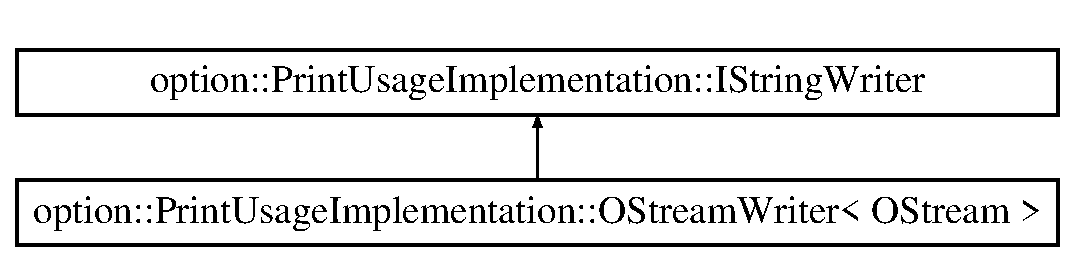
\includegraphics[height=2.000000cm]{structoption_1_1PrintUsageImplementation_1_1OStreamWriter}
\end{center}
\end{figure}
\subsection*{Public Member Functions}
\begin{DoxyCompactItemize}
\item 
\mbox{\Hypertarget{structoption_1_1PrintUsageImplementation_1_1OStreamWriter_a323890fba123ad476fa2471029fc7b23}\label{structoption_1_1PrintUsageImplementation_1_1OStreamWriter_a323890fba123ad476fa2471029fc7b23}} 
virtual void \hyperlink{structoption_1_1PrintUsageImplementation_1_1OStreamWriter_a323890fba123ad476fa2471029fc7b23}{operator()} (const char $\ast$str, int size)
\begin{DoxyCompactList}\small\item\em Writes the given number of chars beginning at the given pointer somewhere. \end{DoxyCompactList}\item 
\mbox{\Hypertarget{structoption_1_1PrintUsageImplementation_1_1OStreamWriter_abf38eb181267e96d86de1ea09ad22c3f}\label{structoption_1_1PrintUsageImplementation_1_1OStreamWriter_abf38eb181267e96d86de1ea09ad22c3f}} 
{\bfseries O\+Stream\+Writer} (O\+Stream \&o)
\end{DoxyCompactItemize}
\subsection*{Public Attributes}
\begin{DoxyCompactItemize}
\item 
\mbox{\Hypertarget{structoption_1_1PrintUsageImplementation_1_1OStreamWriter_a9b808696e204a834acd4362c62b9f4c1}\label{structoption_1_1PrintUsageImplementation_1_1OStreamWriter_a9b808696e204a834acd4362c62b9f4c1}} 
O\+Stream \& {\bfseries ostream}
\end{DoxyCompactItemize}


The documentation for this struct was generated from the following file\+:\begin{DoxyCompactItemize}
\item 
headers/\hyperlink{optionparser_8hpp}{optionparser.\+hpp}\end{DoxyCompactItemize}

\hypertarget{classoption_1_1Parser}{}\section{option\+:\+:Parser Class Reference}
\label{classoption_1_1Parser}\index{option\+::\+Parser@{option\+::\+Parser}}


Checks argument vectors for validity and parses them into data structures that are easier to work with.  




{\ttfamily \#include $<$optionparser.\+hpp$>$}

\subsection*{Classes}
\begin{DoxyCompactItemize}
\item 
struct \hyperlink{structoption_1_1Parser_1_1Action}{Action}
\item 
class \hyperlink{classoption_1_1Parser_1_1StoreOptionAction}{Store\+Option\+Action}
\end{DoxyCompactItemize}
\subsection*{Public Member Functions}
\begin{DoxyCompactItemize}
\item 
\mbox{\Hypertarget{classoption_1_1Parser_a895e9a1db19f1a026ee6a7412de17d04}\label{classoption_1_1Parser_a895e9a1db19f1a026ee6a7412de17d04}} 
\hyperlink{classoption_1_1Parser_a895e9a1db19f1a026ee6a7412de17d04}{Parser} ()
\begin{DoxyCompactList}\small\item\em Creates a new \hyperlink{classoption_1_1Parser}{Parser}. \end{DoxyCompactList}\item 
\hyperlink{classoption_1_1Parser_aa747e9792c9c08ede32b6c323438db71}{Parser} (bool gnu, const \hyperlink{structoption_1_1Descriptor}{Descriptor} usage\mbox{[}$\,$\mbox{]}, int argc, const char $\ast$$\ast$argv, \hyperlink{classoption_1_1Option}{Option} options\mbox{[}$\,$\mbox{]}, \hyperlink{classoption_1_1Option}{Option} buffer\mbox{[}$\,$\mbox{]}, int min\+\_\+abbr\+\_\+len=0, bool single\+\_\+minus\+\_\+longopt=false, int bufmax=-\/1)
\begin{DoxyCompactList}\small\item\em Creates a new \hyperlink{classoption_1_1Parser}{Parser} and immediately parses the given argument vector. \end{DoxyCompactList}\item 
\mbox{\Hypertarget{classoption_1_1Parser_a78b4c7d73fff17204dd908b1b167dec9}\label{classoption_1_1Parser_a78b4c7d73fff17204dd908b1b167dec9}} 
\hyperlink{classoption_1_1Parser_a78b4c7d73fff17204dd908b1b167dec9}{Parser} (bool gnu, const \hyperlink{structoption_1_1Descriptor}{Descriptor} usage\mbox{[}$\,$\mbox{]}, int argc, char $\ast$$\ast$argv, \hyperlink{classoption_1_1Option}{Option} options\mbox{[}$\,$\mbox{]}, \hyperlink{classoption_1_1Option}{Option} buffer\mbox{[}$\,$\mbox{]}, int min\+\_\+abbr\+\_\+len=0, bool single\+\_\+minus\+\_\+longopt=false, int bufmax=-\/1)
\begin{DoxyCompactList}\small\item\em \hyperlink{classoption_1_1Parser}{Parser}(...) with non-\/const argv. \end{DoxyCompactList}\item 
\mbox{\Hypertarget{classoption_1_1Parser_ae4100da4b662937ead22484e6cfc7cec}\label{classoption_1_1Parser_ae4100da4b662937ead22484e6cfc7cec}} 
\hyperlink{classoption_1_1Parser_ae4100da4b662937ead22484e6cfc7cec}{Parser} (const \hyperlink{structoption_1_1Descriptor}{Descriptor} usage\mbox{[}$\,$\mbox{]}, int argc, const char $\ast$$\ast$argv, \hyperlink{classoption_1_1Option}{Option} options\mbox{[}$\,$\mbox{]}, \hyperlink{classoption_1_1Option}{Option} buffer\mbox{[}$\,$\mbox{]}, int min\+\_\+abbr\+\_\+len=0, bool single\+\_\+minus\+\_\+longopt=false, int bufmax=-\/1)
\begin{DoxyCompactList}\small\item\em P\+O\+S\+IX \hyperlink{classoption_1_1Parser}{Parser}(...) (gnu==false). \end{DoxyCompactList}\item 
\mbox{\Hypertarget{classoption_1_1Parser_a23ee244634a38d05f6c4cb1e3692a8a9}\label{classoption_1_1Parser_a23ee244634a38d05f6c4cb1e3692a8a9}} 
\hyperlink{classoption_1_1Parser_a23ee244634a38d05f6c4cb1e3692a8a9}{Parser} (const \hyperlink{structoption_1_1Descriptor}{Descriptor} usage\mbox{[}$\,$\mbox{]}, int argc, char $\ast$$\ast$argv, \hyperlink{classoption_1_1Option}{Option} options\mbox{[}$\,$\mbox{]}, \hyperlink{classoption_1_1Option}{Option} buffer\mbox{[}$\,$\mbox{]}, int min\+\_\+abbr\+\_\+len=0, bool single\+\_\+minus\+\_\+longopt=false, int bufmax=-\/1)
\begin{DoxyCompactList}\small\item\em P\+O\+S\+IX \hyperlink{classoption_1_1Parser}{Parser}(...) (gnu==false) with non-\/const argv. \end{DoxyCompactList}\item 
void \hyperlink{classoption_1_1Parser_a6e0b5778d1cfbd6cd51240e74d01e138}{parse} (bool gnu, const \hyperlink{structoption_1_1Descriptor}{Descriptor} usage\mbox{[}$\,$\mbox{]}, int argc, const char $\ast$$\ast$argv, \hyperlink{classoption_1_1Option}{Option} options\mbox{[}$\,$\mbox{]}, \hyperlink{classoption_1_1Option}{Option} buffer\mbox{[}$\,$\mbox{]}, int min\+\_\+abbr\+\_\+len=0, bool single\+\_\+minus\+\_\+longopt=false, int bufmax=-\/1)
\begin{DoxyCompactList}\small\item\em Parses the given argument vector. \end{DoxyCompactList}\item 
\mbox{\Hypertarget{classoption_1_1Parser_ab26280e3b2ebc2f2fc4ed8b3b1e2a39c}\label{classoption_1_1Parser_ab26280e3b2ebc2f2fc4ed8b3b1e2a39c}} 
void \hyperlink{classoption_1_1Parser_ab26280e3b2ebc2f2fc4ed8b3b1e2a39c}{parse} (bool gnu, const \hyperlink{structoption_1_1Descriptor}{Descriptor} usage\mbox{[}$\,$\mbox{]}, int argc, char $\ast$$\ast$argv, \hyperlink{classoption_1_1Option}{Option} options\mbox{[}$\,$\mbox{]}, \hyperlink{classoption_1_1Option}{Option} buffer\mbox{[}$\,$\mbox{]}, int min\+\_\+abbr\+\_\+len=0, bool single\+\_\+minus\+\_\+longopt=false, int bufmax=-\/1)
\begin{DoxyCompactList}\small\item\em \hyperlink{classoption_1_1Parser_a6e0b5778d1cfbd6cd51240e74d01e138}{parse()} with non-\/const argv. \end{DoxyCompactList}\item 
\mbox{\Hypertarget{classoption_1_1Parser_a41885a7308249c8532714e15b36106bd}\label{classoption_1_1Parser_a41885a7308249c8532714e15b36106bd}} 
void \hyperlink{classoption_1_1Parser_a41885a7308249c8532714e15b36106bd}{parse} (const \hyperlink{structoption_1_1Descriptor}{Descriptor} usage\mbox{[}$\,$\mbox{]}, int argc, const char $\ast$$\ast$argv, \hyperlink{classoption_1_1Option}{Option} options\mbox{[}$\,$\mbox{]}, \hyperlink{classoption_1_1Option}{Option} buffer\mbox{[}$\,$\mbox{]}, int min\+\_\+abbr\+\_\+len=0, bool single\+\_\+minus\+\_\+longopt=false, int bufmax=-\/1)
\begin{DoxyCompactList}\small\item\em P\+O\+S\+IX \hyperlink{classoption_1_1Parser_a6e0b5778d1cfbd6cd51240e74d01e138}{parse()} (gnu==false). \end{DoxyCompactList}\item 
\mbox{\Hypertarget{classoption_1_1Parser_ad40585faa23a97a186cf9a45b8c2b42b}\label{classoption_1_1Parser_ad40585faa23a97a186cf9a45b8c2b42b}} 
void \hyperlink{classoption_1_1Parser_ad40585faa23a97a186cf9a45b8c2b42b}{parse} (const \hyperlink{structoption_1_1Descriptor}{Descriptor} usage\mbox{[}$\,$\mbox{]}, int argc, char $\ast$$\ast$argv, \hyperlink{classoption_1_1Option}{Option} options\mbox{[}$\,$\mbox{]}, \hyperlink{classoption_1_1Option}{Option} buffer\mbox{[}$\,$\mbox{]}, int min\+\_\+abbr\+\_\+len=0, bool single\+\_\+minus\+\_\+longopt=false, int bufmax=-\/1)
\begin{DoxyCompactList}\small\item\em P\+O\+S\+IX \hyperlink{classoption_1_1Parser_a6e0b5778d1cfbd6cd51240e74d01e138}{parse()} (gnu==false) with non-\/const argv. \end{DoxyCompactList}\item 
int \hyperlink{classoption_1_1Parser_aee62badd2a19a5b88cbc4a9b11813b82}{options\+Count} ()
\begin{DoxyCompactList}\small\item\em Returns the number of valid \hyperlink{classoption_1_1Option}{Option} objects in {\ttfamily buffer}\mbox{[}\mbox{]}. \end{DoxyCompactList}\item 
int \hyperlink{classoption_1_1Parser_aa64a6a7c196993a1b20d48e8ddd12a34}{non\+Options\+Count} ()
\begin{DoxyCompactList}\small\item\em Returns the number of non-\/option arguments that remained at the end of the most recent \hyperlink{classoption_1_1Parser_a6e0b5778d1cfbd6cd51240e74d01e138}{parse()} that actually encountered non-\/option arguments. \end{DoxyCompactList}\item 
const char $\ast$$\ast$ \hyperlink{classoption_1_1Parser_a2c11b050f4248d71758dda52c5f9154d}{non\+Options} ()
\begin{DoxyCompactList}\small\item\em Returns a pointer to an array of non-\/option arguments (only valid if {\ttfamily \hyperlink{classoption_1_1Parser_aa64a6a7c196993a1b20d48e8ddd12a34}{non\+Options\+Count()} $>$0 }). \end{DoxyCompactList}\item 
\mbox{\Hypertarget{classoption_1_1Parser_aeeafbf2892a5aca90b89803b2b1cb031}\label{classoption_1_1Parser_aeeafbf2892a5aca90b89803b2b1cb031}} 
const char $\ast$ \hyperlink{classoption_1_1Parser_aeeafbf2892a5aca90b89803b2b1cb031}{non\+Option} (int i)
\begin{DoxyCompactList}\small\item\em Returns {\bfseries {\ttfamily \hyperlink{classoption_1_1Parser_a2c11b050f4248d71758dda52c5f9154d}{non\+Options()}\mbox{[}i\mbox{]}}} ({\itshape without} checking if i is in range!). \end{DoxyCompactList}\item 
bool \hyperlink{classoption_1_1Parser_a2caa149140067b4d13e4d7a104bb3090}{error} ()
\begin{DoxyCompactList}\small\item\em Returns {\ttfamily true} if an unrecoverable error occurred while parsing options. \end{DoxyCompactList}\end{DoxyCompactItemize}
\subsection*{Friends}
\begin{DoxyCompactItemize}
\item 
\mbox{\Hypertarget{classoption_1_1Parser_a7183dc3501d1c87153f9c0d41f869460}\label{classoption_1_1Parser_a7183dc3501d1c87153f9c0d41f869460}} 
struct {\bfseries Stats}
\end{DoxyCompactItemize}


\subsection{Detailed Description}
Checks argument vectors for validity and parses them into data structures that are easier to work with. 

\begin{DoxyParagraph}{Example\+:}

\begin{DoxyCode}
\textcolor{keywordtype}{int} main(\textcolor{keywordtype}{int} argc, \textcolor{keywordtype}{char}* argv[])
\{
  argc-=(argc>0); argv+=(argc>0); \textcolor{comment}{// skip program name argv[0] if present}
  \hyperlink{structoption_1_1Stats}{option::Stats}  stats(usage, argc, argv);
  \hyperlink{classoption_1_1Option}{option::Option} options[stats.options\_max], buffer[stats.buffer\_max];
  \hyperlink{classoption_1_1Parser}{option::Parser} \hyperlink{classoption_1_1Parser_a6e0b5778d1cfbd6cd51240e74d01e138}{parse}(usage, argc, argv, options, buffer);

  \textcolor{keywordflow}{if} (\hyperlink{classoption_1_1Parser_a6e0b5778d1cfbd6cd51240e74d01e138}{parse}.error())
    \textcolor{keywordflow}{return} 1;

  \textcolor{keywordflow}{if} (options[HELP])
  ...
\end{DoxyCode}
 
\end{DoxyParagraph}


\subsection{Constructor \& Destructor Documentation}
\mbox{\Hypertarget{classoption_1_1Parser_aa747e9792c9c08ede32b6c323438db71}\label{classoption_1_1Parser_aa747e9792c9c08ede32b6c323438db71}} 
\index{option\+::\+Parser@{option\+::\+Parser}!Parser@{Parser}}
\index{Parser@{Parser}!option\+::\+Parser@{option\+::\+Parser}}
\subsubsection{\texorpdfstring{Parser()}{Parser()}}
{\footnotesize\ttfamily option\+::\+Parser\+::\+Parser (\begin{DoxyParamCaption}\item[{bool}]{gnu,  }\item[{const \hyperlink{structoption_1_1Descriptor}{Descriptor}}]{usage\mbox{[}$\,$\mbox{]},  }\item[{int}]{argc,  }\item[{const char $\ast$$\ast$}]{argv,  }\item[{\hyperlink{classoption_1_1Option}{Option}}]{options\mbox{[}$\,$\mbox{]},  }\item[{\hyperlink{classoption_1_1Option}{Option}}]{buffer\mbox{[}$\,$\mbox{]},  }\item[{int}]{min\+\_\+abbr\+\_\+len = {\ttfamily 0},  }\item[{bool}]{single\+\_\+minus\+\_\+longopt = {\ttfamily false},  }\item[{int}]{bufmax = {\ttfamily -\/1} }\end{DoxyParamCaption})\hspace{0.3cm}{\ttfamily [inline]}}



Creates a new \hyperlink{classoption_1_1Parser}{Parser} and immediately parses the given argument vector. 


\begin{DoxyParams}{Parameters}
{\em gnu} & if true, \hyperlink{classoption_1_1Parser_a6e0b5778d1cfbd6cd51240e74d01e138}{parse()} will not stop at the first non-\/option argument. Instead it will reorder arguments so that all non-\/options are at the end. This is the default behaviour of G\+NU getopt() but is not conforming to P\+O\+S\+IX. ~\newline
 Note, that once the argument vector has been reordered, the {\ttfamily gnu} flag will have no further effect on this argument vector. So it is enough to pass {\ttfamily gnu==true} when creating \hyperlink{structoption_1_1Stats}{Stats}. \\
\hline
{\em usage} & Array of \hyperlink{structoption_1_1Descriptor}{Descriptor} objects that describe the options to support. The last entry of this array must have 0 in all fields. \\
\hline
{\em argc} & The number of elements from {\ttfamily argv} that are to be parsed. If you pass -\/1, the number will be determined automatically. In that case the {\ttfamily argv} list must end with a N\+U\+LL pointer. \\
\hline
{\em argv} & The arguments to be parsed. If you pass -\/1 as {\ttfamily argc} the last pointer in the {\ttfamily argv} list must be N\+U\+LL to mark the end. \\
\hline
{\em options} & Each entry is the first element of a linked list of Options. Each new option that is parsed will be appended to the list specified by that \hyperlink{classoption_1_1Option}{Option}\textquotesingle{}s \hyperlink{structoption_1_1Descriptor_a1fee8ac44f529c99ac2b1149b4c391b1}{Descriptor\+::index}. If an entry is not yet used (i.\+e. the \hyperlink{classoption_1_1Option}{Option} is invalid), it will be replaced rather than appended to. ~\newline
 The minimum length of this array is the greatest \hyperlink{structoption_1_1Descriptor_a1fee8ac44f529c99ac2b1149b4c391b1}{Descriptor\+::index} value that occurs in {\ttfamily usage} {\itshape P\+L\+US} O\+NE. \\
\hline
{\em buffer} & Each argument that is successfully parsed (including unknown arguments, if they have a \hyperlink{structoption_1_1Descriptor}{Descriptor} whose Check\+Arg does not return \hyperlink{namespaceoption_aee8c76a07877335762631491e7a5a1a9a9528e32563b795bd2930b12d0a5e382d}{A\+R\+G\+\_\+\+I\+L\+L\+E\+G\+AL}) will be stored in this array. \hyperlink{classoption_1_1Parser_a6e0b5778d1cfbd6cd51240e74d01e138}{parse()} scans the array for the first invalid entry and begins writing at that index. You can pass {\ttfamily bufmax} to limit the number of options stored. \\
\hline
{\em min\+\_\+abbr\+\_\+len} & Passing a value {\ttfamily  min\+\_\+abbr\+\_\+len $>$ 0 } enables abbreviated long options. The parser will match a prefix of a long option as if it was the full long option (e.\+g. {\ttfamily --foob=10} will be interpreted as if it was {\ttfamily --foobar=10} ), as long as the prefix has at least {\ttfamily min\+\_\+abbr\+\_\+len} characters (not counting the {\ttfamily --} ) and is unambiguous. ~\newline
 Be careful if combining {\ttfamily min\+\_\+abbr\+\_\+len=1} with {\ttfamily single\+\_\+minus\+\_\+longopt=true} because the ambiguity check does not consider short options and abbreviated single minus long options will take precedence over short options. \\
\hline
{\em single\+\_\+minus\+\_\+longopt} & Passing {\ttfamily true} for this option allows long options to begin with a single minus. The double minus form will still be recognized. Note that single minus long options take precedence over short options and short option groups. E.\+g. {\ttfamily -\/file} would be interpreted as {\ttfamily --file} and not as {\ttfamily  -\/f -\/i -\/l -\/e } (assuming a long option named {\ttfamily \char`\"{}file\char`\"{}} exists). \\
\hline
{\em bufmax} & The greatest index in the {\ttfamily buffer}\mbox{[}\mbox{]} array that \hyperlink{classoption_1_1Parser_a6e0b5778d1cfbd6cd51240e74d01e138}{parse()} will write to is {\ttfamily bufmax-\/1}. If there are more options, they will be processed (in particular their Check\+Arg will be called) but not stored. ~\newline
 If you used \hyperlink{structoption_1_1Stats_a2c9a7b4174f91ba8bcadaa9ad6f0db06}{Stats\+::buffer\+\_\+max} to dimension this array, you can pass -\/1 (or not pass {\ttfamily bufmax} at all) which tells \hyperlink{classoption_1_1Parser_a6e0b5778d1cfbd6cd51240e74d01e138}{parse()} that the buffer is \char`\"{}large enough\char`\"{}. \\
\hline
\end{DoxyParams}
\begin{DoxyAttention}{Attention}
Remember that {\ttfamily options} and {\ttfamily buffer} store \hyperlink{classoption_1_1Option}{Option} {\itshape objects}, not pointers. Therefore it is not possible for the same object to be in both arrays. For those options that are found in both {\ttfamily buffer}\mbox{[}\mbox{]} and {\ttfamily options}\mbox{[}\mbox{]} the respective objects are independent copies. And only the objects in {\ttfamily options}\mbox{[}\mbox{]} are properly linked via \hyperlink{classoption_1_1Option_a59ae9aed505f4d410633bb36478a32be}{Option\+::next()} and \hyperlink{classoption_1_1Option_a4d12001a91b0b35cf47437d0c60d2b52}{Option\+::prev()}. You can iterate over {\ttfamily buffer}\mbox{[}\mbox{]} to process all options in the order they appear in the argument vector, but if you want access to the other Options with the same \hyperlink{structoption_1_1Descriptor_a1fee8ac44f529c99ac2b1149b4c391b1}{Descriptor\+::index}, then you {\itshape must} access the linked list via {\ttfamily options}\mbox{[}\mbox{]}. You can get the linked list in options from a buffer object via something like {\ttfamily options}\mbox{[}buffer\mbox{[}i\mbox{]}.index()\mbox{]}. 
\end{DoxyAttention}


\subsection{Member Function Documentation}
\mbox{\Hypertarget{classoption_1_1Parser_a2caa149140067b4d13e4d7a104bb3090}\label{classoption_1_1Parser_a2caa149140067b4d13e4d7a104bb3090}} 
\index{option\+::\+Parser@{option\+::\+Parser}!error@{error}}
\index{error@{error}!option\+::\+Parser@{option\+::\+Parser}}
\subsubsection{\texorpdfstring{error()}{error()}}
{\footnotesize\ttfamily bool option\+::\+Parser\+::error (\begin{DoxyParamCaption}{ }\end{DoxyParamCaption})\hspace{0.3cm}{\ttfamily [inline]}}



Returns {\ttfamily true} if an unrecoverable error occurred while parsing options. 

An illegal argument to an option (i.\+e. Check\+Arg returns \hyperlink{namespaceoption_aee8c76a07877335762631491e7a5a1a9a9528e32563b795bd2930b12d0a5e382d}{A\+R\+G\+\_\+\+I\+L\+L\+E\+G\+AL}) is an unrecoverable error that aborts the parse. Unknown options are only an error if their Check\+Arg function returns \hyperlink{namespaceoption_aee8c76a07877335762631491e7a5a1a9a9528e32563b795bd2930b12d0a5e382d}{A\+R\+G\+\_\+\+I\+L\+L\+E\+G\+AL}. Otherwise they are collected. In that case if you want to exit the program if either an illegal argument or an unknown option has been passed, use code like this


\begin{DoxyCode}
\textcolor{keywordflow}{if} (parser.error() || options[UNKNOWN])
  exit(1);
\end{DoxyCode}
 \mbox{\Hypertarget{classoption_1_1Parser_a2c11b050f4248d71758dda52c5f9154d}\label{classoption_1_1Parser_a2c11b050f4248d71758dda52c5f9154d}} 
\index{option\+::\+Parser@{option\+::\+Parser}!non\+Options@{non\+Options}}
\index{non\+Options@{non\+Options}!option\+::\+Parser@{option\+::\+Parser}}
\subsubsection{\texorpdfstring{non\+Options()}{nonOptions()}}
{\footnotesize\ttfamily const char$\ast$$\ast$ option\+::\+Parser\+::non\+Options (\begin{DoxyParamCaption}{ }\end{DoxyParamCaption})\hspace{0.3cm}{\ttfamily [inline]}}



Returns a pointer to an array of non-\/option arguments (only valid if {\ttfamily \hyperlink{classoption_1_1Parser_aa64a6a7c196993a1b20d48e8ddd12a34}{non\+Options\+Count()} $>$0 }). 

\begin{DoxyNote}{Note}
\begin{DoxyItemize}
\item \hyperlink{classoption_1_1Parser_a6e0b5778d1cfbd6cd51240e74d01e138}{parse()} does not copy arguments, so this pointer points into the actual argument vector as passed to \hyperlink{classoption_1_1Parser_a6e0b5778d1cfbd6cd51240e74d01e138}{parse()}. \item As explained at \hyperlink{classoption_1_1Parser_aa64a6a7c196993a1b20d48e8ddd12a34}{non\+Options\+Count()} this pointer is only changed by \hyperlink{classoption_1_1Parser_a6e0b5778d1cfbd6cd51240e74d01e138}{parse()} calls that actually encounter non-\/option arguments. A \hyperlink{classoption_1_1Parser_a6e0b5778d1cfbd6cd51240e74d01e138}{parse()} call that encounters only options, will not change \hyperlink{classoption_1_1Parser_a2c11b050f4248d71758dda52c5f9154d}{non\+Options()}. \end{DoxyItemize}

\end{DoxyNote}
\mbox{\Hypertarget{classoption_1_1Parser_aa64a6a7c196993a1b20d48e8ddd12a34}\label{classoption_1_1Parser_aa64a6a7c196993a1b20d48e8ddd12a34}} 
\index{option\+::\+Parser@{option\+::\+Parser}!non\+Options\+Count@{non\+Options\+Count}}
\index{non\+Options\+Count@{non\+Options\+Count}!option\+::\+Parser@{option\+::\+Parser}}
\subsubsection{\texorpdfstring{non\+Options\+Count()}{nonOptionsCount()}}
{\footnotesize\ttfamily int option\+::\+Parser\+::non\+Options\+Count (\begin{DoxyParamCaption}{ }\end{DoxyParamCaption})\hspace{0.3cm}{\ttfamily [inline]}}



Returns the number of non-\/option arguments that remained at the end of the most recent \hyperlink{classoption_1_1Parser_a6e0b5778d1cfbd6cd51240e74d01e138}{parse()} that actually encountered non-\/option arguments. 

\begin{DoxyNote}{Note}
A \hyperlink{classoption_1_1Parser_a6e0b5778d1cfbd6cd51240e74d01e138}{parse()} that does not encounter non-\/option arguments will leave this value as well as \hyperlink{classoption_1_1Parser_a2c11b050f4248d71758dda52c5f9154d}{non\+Options()} undisturbed. This means you can feed the \hyperlink{classoption_1_1Parser}{Parser} a default argument vector that contains non-\/option arguments (e.\+g. a default filename). Then you feed it the actual arguments from the user. If the user has supplied at least one non-\/option argument, all of the non-\/option arguments from the default disappear and are replaced by the user\textquotesingle{}s non-\/option arguments. However, if the user does not supply any non-\/option arguments the defaults will still be in effect. 
\end{DoxyNote}
\mbox{\Hypertarget{classoption_1_1Parser_aee62badd2a19a5b88cbc4a9b11813b82}\label{classoption_1_1Parser_aee62badd2a19a5b88cbc4a9b11813b82}} 
\index{option\+::\+Parser@{option\+::\+Parser}!options\+Count@{options\+Count}}
\index{options\+Count@{options\+Count}!option\+::\+Parser@{option\+::\+Parser}}
\subsubsection{\texorpdfstring{options\+Count()}{optionsCount()}}
{\footnotesize\ttfamily int option\+::\+Parser\+::options\+Count (\begin{DoxyParamCaption}{ }\end{DoxyParamCaption})\hspace{0.3cm}{\ttfamily [inline]}}



Returns the number of valid \hyperlink{classoption_1_1Option}{Option} objects in {\ttfamily buffer}\mbox{[}\mbox{]}. 

\begin{DoxyNote}{Note}
\begin{DoxyItemize}
\item The returned value always reflects the number of Options in the buffer\mbox{[}\mbox{]} array used for the most recent call to \hyperlink{classoption_1_1Parser_a6e0b5778d1cfbd6cd51240e74d01e138}{parse()}. \item The count (and the buffer\mbox{[}\mbox{]}) includes unknown options if they are collected (see \hyperlink{structoption_1_1Descriptor_a470c449dfa894c9bfda2dae026142b4b}{Descriptor\+::longopt}). \end{DoxyItemize}

\end{DoxyNote}
\mbox{\Hypertarget{classoption_1_1Parser_a6e0b5778d1cfbd6cd51240e74d01e138}\label{classoption_1_1Parser_a6e0b5778d1cfbd6cd51240e74d01e138}} 
\index{option\+::\+Parser@{option\+::\+Parser}!parse@{parse}}
\index{parse@{parse}!option\+::\+Parser@{option\+::\+Parser}}
\subsubsection{\texorpdfstring{parse()}{parse()}}
{\footnotesize\ttfamily void option\+::\+Parser\+::parse (\begin{DoxyParamCaption}\item[{bool}]{gnu,  }\item[{const \hyperlink{structoption_1_1Descriptor}{Descriptor}}]{usage\mbox{[}$\,$\mbox{]},  }\item[{int}]{argc,  }\item[{const char $\ast$$\ast$}]{argv,  }\item[{\hyperlink{classoption_1_1Option}{Option}}]{options\mbox{[}$\,$\mbox{]},  }\item[{\hyperlink{classoption_1_1Option}{Option}}]{buffer\mbox{[}$\,$\mbox{]},  }\item[{int}]{min\+\_\+abbr\+\_\+len = {\ttfamily 0},  }\item[{bool}]{single\+\_\+minus\+\_\+longopt = {\ttfamily false},  }\item[{int}]{bufmax = {\ttfamily -\/1} }\end{DoxyParamCaption})\hspace{0.3cm}{\ttfamily [inline]}}



Parses the given argument vector. 


\begin{DoxyParams}{Parameters}
{\em gnu} & if true, \hyperlink{classoption_1_1Parser_a6e0b5778d1cfbd6cd51240e74d01e138}{parse()} will not stop at the first non-\/option argument. Instead it will reorder arguments so that all non-\/options are at the end. This is the default behaviour of G\+NU getopt() but is not conforming to P\+O\+S\+IX. ~\newline
 Note, that once the argument vector has been reordered, the {\ttfamily gnu} flag will have no further effect on this argument vector. So it is enough to pass {\ttfamily gnu==true} when creating \hyperlink{structoption_1_1Stats}{Stats}. \\
\hline
{\em usage} & Array of \hyperlink{structoption_1_1Descriptor}{Descriptor} objects that describe the options to support. The last entry of this array must have 0 in all fields. \\
\hline
{\em argc} & The number of elements from {\ttfamily argv} that are to be parsed. If you pass -\/1, the number will be determined automatically. In that case the {\ttfamily argv} list must end with a N\+U\+LL pointer. \\
\hline
{\em argv} & The arguments to be parsed. If you pass -\/1 as {\ttfamily argc} the last pointer in the {\ttfamily argv} list must be N\+U\+LL to mark the end. \\
\hline
{\em options} & Each entry is the first element of a linked list of Options. Each new option that is parsed will be appended to the list specified by that \hyperlink{classoption_1_1Option}{Option}\textquotesingle{}s \hyperlink{structoption_1_1Descriptor_a1fee8ac44f529c99ac2b1149b4c391b1}{Descriptor\+::index}. If an entry is not yet used (i.\+e. the \hyperlink{classoption_1_1Option}{Option} is invalid), it will be replaced rather than appended to. ~\newline
 The minimum length of this array is the greatest \hyperlink{structoption_1_1Descriptor_a1fee8ac44f529c99ac2b1149b4c391b1}{Descriptor\+::index} value that occurs in {\ttfamily usage} {\itshape P\+L\+US} O\+NE. \\
\hline
{\em buffer} & Each argument that is successfully parsed (including unknown arguments, if they have a \hyperlink{structoption_1_1Descriptor}{Descriptor} whose Check\+Arg does not return \hyperlink{namespaceoption_aee8c76a07877335762631491e7a5a1a9a9528e32563b795bd2930b12d0a5e382d}{A\+R\+G\+\_\+\+I\+L\+L\+E\+G\+AL}) will be stored in this array. \hyperlink{classoption_1_1Parser_a6e0b5778d1cfbd6cd51240e74d01e138}{parse()} scans the array for the first invalid entry and begins writing at that index. You can pass {\ttfamily bufmax} to limit the number of options stored. \\
\hline
{\em min\+\_\+abbr\+\_\+len} & Passing a value {\ttfamily  min\+\_\+abbr\+\_\+len $>$ 0 } enables abbreviated long options. The parser will match a prefix of a long option as if it was the full long option (e.\+g. {\ttfamily --foob=10} will be interpreted as if it was {\ttfamily --foobar=10} ), as long as the prefix has at least {\ttfamily min\+\_\+abbr\+\_\+len} characters (not counting the {\ttfamily --} ) and is unambiguous. ~\newline
 Be careful if combining {\ttfamily min\+\_\+abbr\+\_\+len=1} with {\ttfamily single\+\_\+minus\+\_\+longopt=true} because the ambiguity check does not consider short options and abbreviated single minus long options will take precedence over short options. \\
\hline
{\em single\+\_\+minus\+\_\+longopt} & Passing {\ttfamily true} for this option allows long options to begin with a single minus. The double minus form will still be recognized. Note that single minus long options take precedence over short options and short option groups. E.\+g. {\ttfamily -\/file} would be interpreted as {\ttfamily --file} and not as {\ttfamily  -\/f -\/i -\/l -\/e } (assuming a long option named {\ttfamily \char`\"{}file\char`\"{}} exists). \\
\hline
{\em bufmax} & The greatest index in the {\ttfamily buffer}\mbox{[}\mbox{]} array that \hyperlink{classoption_1_1Parser_a6e0b5778d1cfbd6cd51240e74d01e138}{parse()} will write to is {\ttfamily bufmax-\/1}. If there are more options, they will be processed (in particular their Check\+Arg will be called) but not stored. ~\newline
 If you used \hyperlink{structoption_1_1Stats_a2c9a7b4174f91ba8bcadaa9ad6f0db06}{Stats\+::buffer\+\_\+max} to dimension this array, you can pass -\/1 (or not pass {\ttfamily bufmax} at all) which tells \hyperlink{classoption_1_1Parser_a6e0b5778d1cfbd6cd51240e74d01e138}{parse()} that the buffer is \char`\"{}large enough\char`\"{}. \\
\hline
\end{DoxyParams}
\begin{DoxyAttention}{Attention}
Remember that {\ttfamily options} and {\ttfamily buffer} store \hyperlink{classoption_1_1Option}{Option} {\itshape objects}, not pointers. Therefore it is not possible for the same object to be in both arrays. For those options that are found in both {\ttfamily buffer}\mbox{[}\mbox{]} and {\ttfamily options}\mbox{[}\mbox{]} the respective objects are independent copies. And only the objects in {\ttfamily options}\mbox{[}\mbox{]} are properly linked via \hyperlink{classoption_1_1Option_a59ae9aed505f4d410633bb36478a32be}{Option\+::next()} and \hyperlink{classoption_1_1Option_a4d12001a91b0b35cf47437d0c60d2b52}{Option\+::prev()}. You can iterate over {\ttfamily buffer}\mbox{[}\mbox{]} to process all options in the order they appear in the argument vector, but if you want access to the other Options with the same \hyperlink{structoption_1_1Descriptor_a1fee8ac44f529c99ac2b1149b4c391b1}{Descriptor\+::index}, then you {\itshape must} access the linked list via {\ttfamily options}\mbox{[}\mbox{]}. You can get the linked list in options from a buffer object via something like {\ttfamily options}\mbox{[}buffer\mbox{[}i\mbox{]}.index()\mbox{]}. 
\end{DoxyAttention}


The documentation for this class was generated from the following file\+:\begin{DoxyCompactItemize}
\item 
headers/\hyperlink{optionparser_8hpp}{optionparser.\+hpp}\end{DoxyCompactItemize}

\hypertarget{structoption_1_1PrintUsageImplementation}{}\section{option\+:\+:Print\+Usage\+Implementation Struct Reference}
\label{structoption_1_1PrintUsageImplementation}\index{option\+::\+Print\+Usage\+Implementation@{option\+::\+Print\+Usage\+Implementation}}
\subsection*{Classes}
\begin{DoxyCompactItemize}
\item 
struct \hyperlink{structoption_1_1PrintUsageImplementation_1_1FunctionWriter}{Function\+Writer}
\item 
struct \hyperlink{structoption_1_1PrintUsageImplementation_1_1IStringWriter}{I\+String\+Writer}
\item 
class \hyperlink{classoption_1_1PrintUsageImplementation_1_1LinePartIterator}{Line\+Part\+Iterator}
\item 
class \hyperlink{classoption_1_1PrintUsageImplementation_1_1LineWrapper}{Line\+Wrapper}
\item 
struct \hyperlink{structoption_1_1PrintUsageImplementation_1_1OStreamWriter}{O\+Stream\+Writer}
\item 
struct \hyperlink{structoption_1_1PrintUsageImplementation_1_1StreamWriter}{Stream\+Writer}
\item 
struct \hyperlink{structoption_1_1PrintUsageImplementation_1_1SyscallWriter}{Syscall\+Writer}
\item 
struct \hyperlink{structoption_1_1PrintUsageImplementation_1_1TemporaryWriter}{Temporary\+Writer}
\end{DoxyCompactItemize}
\subsection*{Static Public Member Functions}
\begin{DoxyCompactItemize}
\item 
\mbox{\Hypertarget{structoption_1_1PrintUsageImplementation_a0680dd84366df82398e30e4ccbd27ac0}\label{structoption_1_1PrintUsageImplementation_a0680dd84366df82398e30e4ccbd27ac0}} 
static void {\bfseries upmax} (int \&i1, int i2)
\item 
\mbox{\Hypertarget{structoption_1_1PrintUsageImplementation_a4136c574bba35ea1f478e0b6d7022367}\label{structoption_1_1PrintUsageImplementation_a4136c574bba35ea1f478e0b6d7022367}} 
static void {\bfseries indent} (\hyperlink{structoption_1_1PrintUsageImplementation_1_1IStringWriter}{I\+String\+Writer} \&write, int \&x, int want\+\_\+x)
\item 
static bool \hyperlink{structoption_1_1PrintUsageImplementation_a41bfaabdf21e68877f3030d36acc0798}{is\+Wide\+Char} (unsigned ch)
\begin{DoxyCompactList}\small\item\em Returns true if ch is the unicode code point of a wide character. \end{DoxyCompactList}\item 
\mbox{\Hypertarget{structoption_1_1PrintUsageImplementation_ab38c4198c5cccea2ccd992c8e014df70}\label{structoption_1_1PrintUsageImplementation_ab38c4198c5cccea2ccd992c8e014df70}} 
static void {\bfseries print\+Usage} (\hyperlink{structoption_1_1PrintUsageImplementation_1_1IStringWriter}{I\+String\+Writer} \&write, const \hyperlink{structoption_1_1Descriptor}{Descriptor} usage\mbox{[}$\,$\mbox{]}, int width=80, int last\+\_\+column\+\_\+min\+\_\+percent=50, int last\+\_\+column\+\_\+own\+\_\+line\+\_\+max\+\_\+percent=75)
\end{DoxyCompactItemize}


\subsection{Member Function Documentation}
\mbox{\Hypertarget{structoption_1_1PrintUsageImplementation_a41bfaabdf21e68877f3030d36acc0798}\label{structoption_1_1PrintUsageImplementation_a41bfaabdf21e68877f3030d36acc0798}} 
\index{option\+::\+Print\+Usage\+Implementation@{option\+::\+Print\+Usage\+Implementation}!is\+Wide\+Char@{is\+Wide\+Char}}
\index{is\+Wide\+Char@{is\+Wide\+Char}!option\+::\+Print\+Usage\+Implementation@{option\+::\+Print\+Usage\+Implementation}}
\subsubsection{\texorpdfstring{is\+Wide\+Char()}{isWideChar()}}
{\footnotesize\ttfamily static bool option\+::\+Print\+Usage\+Implementation\+::is\+Wide\+Char (\begin{DoxyParamCaption}\item[{unsigned}]{ch }\end{DoxyParamCaption})\hspace{0.3cm}{\ttfamily [inline]}, {\ttfamily [static]}}



Returns true if ch is the unicode code point of a wide character. 

\begin{DoxyNote}{Note}
The following character ranges are treated as wide 
\begin{DoxyCode}
1100..115F
2329..232A  (just 2 characters!)
2E80..A4C6  except \textcolor{keywordflow}{for} 303F
A960..A97C
AC00..D7FB
F900..FAFF
FE10..FE6B
FF01..FF60
FFE0..FFE6
1B000......
\end{DoxyCode}
 
\end{DoxyNote}


The documentation for this struct was generated from the following file\+:\begin{DoxyCompactItemize}
\item 
headers/\hyperlink{optionparser_8hpp}{optionparser.\+hpp}\end{DoxyCompactItemize}

\hypertarget{classRelFrequency}{}\section{Rel\+Frequency Class Reference}
\label{classRelFrequency}\index{Rel\+Frequency@{Rel\+Frequency}}
\subsection*{Public Member Functions}
\begin{DoxyCompactItemize}
\item 
\mbox{\Hypertarget{classRelFrequency_aee770cbb787b7ddb411d86286e173c54}\label{classRelFrequency_aee770cbb787b7ddb411d86286e173c54}} 
{\bfseries Rel\+Frequency} (map$<$ char, double $>$)
\item 
\mbox{\Hypertarget{classRelFrequency_a34f54589602ae3d3358c4fc3c5ee715e}\label{classRelFrequency_a34f54589602ae3d3358c4fc3c5ee715e}} 
map$<$ char, double $>$ {\bfseries get\+Symbol\+Frequency} ()
\item 
\mbox{\Hypertarget{classRelFrequency_a4fbb38610164cf71b9f907a37e1ee799}\label{classRelFrequency_a4fbb38610164cf71b9f907a37e1ee799}} 
double {\bfseries get\+Symbol\+Frequency} (char)
\item 
\mbox{\Hypertarget{classRelFrequency_aafe45f13cb37a2036a41ad63a7165b5d}\label{classRelFrequency_aafe45f13cb37a2036a41ad63a7165b5d}} 
void {\bfseries print\+Frequencies} ()
\item 
\mbox{\Hypertarget{classRelFrequency_a4a46dc5717a5e58dbdb15279f2d62607}\label{classRelFrequency_a4a46dc5717a5e58dbdb15279f2d62607}} 
double {\bfseries compare} (\hyperlink{classRelFrequency}{Rel\+Frequency})
\end{DoxyCompactItemize}
\subsection*{Static Public Member Functions}
\begin{DoxyCompactItemize}
\item 
\mbox{\Hypertarget{classRelFrequency_aeda20735e026cfa333b283d2d1242aad}\label{classRelFrequency_aeda20735e026cfa333b283d2d1242aad}} 
static \hyperlink{classRelFrequency}{Rel\+Frequency} {\bfseries Frequency\+From\+C\+SV} (string)
\item 
\mbox{\Hypertarget{classRelFrequency_ad0ce5a278daab2b6582071e31bb6caac}\label{classRelFrequency_ad0ce5a278daab2b6582071e31bb6caac}} 
static \hyperlink{classRelFrequency}{Rel\+Frequency} {\bfseries Frequency\+From\+String} (string)
\item 
\mbox{\Hypertarget{classRelFrequency_a43fcccc59922592eac3981a777841df4}\label{classRelFrequency_a43fcccc59922592eac3981a777841df4}} 
static \hyperlink{classRelFrequency}{Rel\+Frequency} {\bfseries Frequency\+From\+File} (string)
\end{DoxyCompactItemize}


The documentation for this class was generated from the following files\+:\begin{DoxyCompactItemize}
\item 
headers/\hyperlink{Frequency_8hpp}{Frequency.\+hpp}\item 
sources/\hyperlink{Frequency_8cpp}{Frequency.\+cpp}\end{DoxyCompactItemize}

\hypertarget{structoption_1_1Stats}{}\section{option\+:\+:Stats Struct Reference}
\label{structoption_1_1Stats}\index{option\+::\+Stats@{option\+::\+Stats}}


Determines the minimum lengths of the buffer and options arrays used for \hyperlink{classoption_1_1Parser}{Parser}.  




{\ttfamily \#include $<$optionparser.\+hpp$>$}

\subsection*{Classes}
\begin{DoxyCompactItemize}
\item 
class \hyperlink{classoption_1_1Stats_1_1CountOptionsAction}{Count\+Options\+Action}
\end{DoxyCompactItemize}
\subsection*{Public Member Functions}
\begin{DoxyCompactItemize}
\item 
\mbox{\Hypertarget{structoption_1_1Stats_a8660722c76e65d9328313fb360bdd282}\label{structoption_1_1Stats_a8660722c76e65d9328313fb360bdd282}} 
\hyperlink{structoption_1_1Stats_a8660722c76e65d9328313fb360bdd282}{Stats} ()
\begin{DoxyCompactList}\small\item\em Creates a \hyperlink{structoption_1_1Stats}{Stats} object with counts set to 1 (for the sentinel element). \end{DoxyCompactList}\item 
\hyperlink{structoption_1_1Stats_a71373ec2b28842f45593e4405f7bc8ec}{Stats} (bool gnu, const \hyperlink{structoption_1_1Descriptor}{Descriptor} usage\mbox{[}$\,$\mbox{]}, int argc, const char $\ast$$\ast$argv, int min\+\_\+abbr\+\_\+len=0, bool single\+\_\+minus\+\_\+longopt=false)
\begin{DoxyCompactList}\small\item\em Creates a new \hyperlink{structoption_1_1Stats}{Stats} object and immediately updates it for the given {\ttfamily usage} and argument vector. You may pass 0 for {\ttfamily argc} and/or {\ttfamily argv}, if you just want to update \hyperlink{structoption_1_1Stats_a8121787feb1c7db84fca3ccb012b0473}{options\+\_\+max}. \end{DoxyCompactList}\item 
\mbox{\Hypertarget{structoption_1_1Stats_a43ec104fdb0b8ae6148d04f3ad3d3a75}\label{structoption_1_1Stats_a43ec104fdb0b8ae6148d04f3ad3d3a75}} 
\hyperlink{structoption_1_1Stats_a43ec104fdb0b8ae6148d04f3ad3d3a75}{Stats} (bool gnu, const \hyperlink{structoption_1_1Descriptor}{Descriptor} usage\mbox{[}$\,$\mbox{]}, int argc, char $\ast$$\ast$argv, int min\+\_\+abbr\+\_\+len=0, bool single\+\_\+minus\+\_\+longopt=false)
\begin{DoxyCompactList}\small\item\em \hyperlink{structoption_1_1Stats}{Stats}(...) with non-\/const argv. \end{DoxyCompactList}\item 
\mbox{\Hypertarget{structoption_1_1Stats_ab5cafb7127099ef60cfb4cea205ad617}\label{structoption_1_1Stats_ab5cafb7127099ef60cfb4cea205ad617}} 
\hyperlink{structoption_1_1Stats_ab5cafb7127099ef60cfb4cea205ad617}{Stats} (const \hyperlink{structoption_1_1Descriptor}{Descriptor} usage\mbox{[}$\,$\mbox{]}, int argc, const char $\ast$$\ast$argv, int min\+\_\+abbr\+\_\+len=0, bool single\+\_\+minus\+\_\+longopt=false)
\begin{DoxyCompactList}\small\item\em P\+O\+S\+IX \hyperlink{structoption_1_1Stats}{Stats}(...) (gnu==false). \end{DoxyCompactList}\item 
\mbox{\Hypertarget{structoption_1_1Stats_a9b8b4f275efaac6a509df75179929c70}\label{structoption_1_1Stats_a9b8b4f275efaac6a509df75179929c70}} 
\hyperlink{structoption_1_1Stats_a9b8b4f275efaac6a509df75179929c70}{Stats} (const \hyperlink{structoption_1_1Descriptor}{Descriptor} usage\mbox{[}$\,$\mbox{]}, int argc, char $\ast$$\ast$argv, int min\+\_\+abbr\+\_\+len=0, bool single\+\_\+minus\+\_\+longopt=false)
\begin{DoxyCompactList}\small\item\em P\+O\+S\+IX \hyperlink{structoption_1_1Stats}{Stats}(...) (gnu==false) with non-\/const argv. \end{DoxyCompactList}\item 
void \hyperlink{structoption_1_1Stats_aa77e2a8b1704527d2d087820f4456143}{add} (bool gnu, const \hyperlink{structoption_1_1Descriptor}{Descriptor} usage\mbox{[}$\,$\mbox{]}, int argc, const char $\ast$$\ast$argv, int min\+\_\+abbr\+\_\+len=0, bool single\+\_\+minus\+\_\+longopt=false)
\begin{DoxyCompactList}\small\item\em Updates this \hyperlink{structoption_1_1Stats}{Stats} object for the given {\ttfamily usage} and argument vector. You may pass 0 for {\ttfamily argc} and/or {\ttfamily argv}, if you just want to update \hyperlink{structoption_1_1Stats_a8121787feb1c7db84fca3ccb012b0473}{options\+\_\+max}. \end{DoxyCompactList}\item 
\mbox{\Hypertarget{structoption_1_1Stats_a2aa7bc64a85dcd9c59576f6a11c2b747}\label{structoption_1_1Stats_a2aa7bc64a85dcd9c59576f6a11c2b747}} 
void \hyperlink{structoption_1_1Stats_a2aa7bc64a85dcd9c59576f6a11c2b747}{add} (bool gnu, const \hyperlink{structoption_1_1Descriptor}{Descriptor} usage\mbox{[}$\,$\mbox{]}, int argc, char $\ast$$\ast$argv, int min\+\_\+abbr\+\_\+len=0, bool single\+\_\+minus\+\_\+longopt=false)
\begin{DoxyCompactList}\small\item\em \hyperlink{structoption_1_1Stats_aa77e2a8b1704527d2d087820f4456143}{add()} with non-\/const argv. \end{DoxyCompactList}\item 
\mbox{\Hypertarget{structoption_1_1Stats_a4fc47be5db7f52016e3142a9b9dd0d1e}\label{structoption_1_1Stats_a4fc47be5db7f52016e3142a9b9dd0d1e}} 
void \hyperlink{structoption_1_1Stats_a4fc47be5db7f52016e3142a9b9dd0d1e}{add} (const \hyperlink{structoption_1_1Descriptor}{Descriptor} usage\mbox{[}$\,$\mbox{]}, int argc, const char $\ast$$\ast$argv, int min\+\_\+abbr\+\_\+len=0, bool single\+\_\+minus\+\_\+longopt=false)
\begin{DoxyCompactList}\small\item\em P\+O\+S\+IX \hyperlink{structoption_1_1Stats_aa77e2a8b1704527d2d087820f4456143}{add()} (gnu==false). \end{DoxyCompactList}\item 
\mbox{\Hypertarget{structoption_1_1Stats_ad659604438f79c79f5bc009f2a16ca92}\label{structoption_1_1Stats_ad659604438f79c79f5bc009f2a16ca92}} 
void \hyperlink{structoption_1_1Stats_ad659604438f79c79f5bc009f2a16ca92}{add} (const \hyperlink{structoption_1_1Descriptor}{Descriptor} usage\mbox{[}$\,$\mbox{]}, int argc, char $\ast$$\ast$argv, int min\+\_\+abbr\+\_\+len=0, bool single\+\_\+minus\+\_\+longopt=false)
\begin{DoxyCompactList}\small\item\em P\+O\+S\+IX \hyperlink{structoption_1_1Stats_aa77e2a8b1704527d2d087820f4456143}{add()} (gnu==false) with non-\/const argv. \end{DoxyCompactList}\end{DoxyCompactItemize}
\subsection*{Public Attributes}
\begin{DoxyCompactItemize}
\item 
unsigned \hyperlink{structoption_1_1Stats_a2c9a7b4174f91ba8bcadaa9ad6f0db06}{buffer\+\_\+max}
\begin{DoxyCompactList}\small\item\em Number of elements needed for a {\ttfamily buffer}\mbox{[}\mbox{]} array to be used for \hyperlink{classoption_1_1Parser_a6e0b5778d1cfbd6cd51240e74d01e138}{parsing} the same argument vectors that were fed into this \hyperlink{structoption_1_1Stats}{Stats} object. \end{DoxyCompactList}\item 
unsigned \hyperlink{structoption_1_1Stats_a8121787feb1c7db84fca3ccb012b0473}{options\+\_\+max}
\begin{DoxyCompactList}\small\item\em Number of elements needed for an {\ttfamily options}\mbox{[}\mbox{]} array to be used for \hyperlink{classoption_1_1Parser_a6e0b5778d1cfbd6cd51240e74d01e138}{parsing} the same argument vectors that were fed into this \hyperlink{structoption_1_1Stats}{Stats} object. \end{DoxyCompactList}\end{DoxyCompactItemize}


\subsection{Detailed Description}
Determines the minimum lengths of the buffer and options arrays used for \hyperlink{classoption_1_1Parser}{Parser}. 

Because \hyperlink{classoption_1_1Parser}{Parser} doesn\textquotesingle{}t use dynamic memory its output arrays have to be pre-\/allocated. If you don\textquotesingle{}t want to use fixed size arrays (which may turn out too small, causing command line arguments to be dropped), you can use \hyperlink{structoption_1_1Stats}{Stats} to determine the correct sizes. \hyperlink{structoption_1_1Stats}{Stats} work cumulative. You can first pass in your default options and then the real options and afterwards the counts will reflect the union. 

\subsection{Constructor \& Destructor Documentation}
\mbox{\Hypertarget{structoption_1_1Stats_a71373ec2b28842f45593e4405f7bc8ec}\label{structoption_1_1Stats_a71373ec2b28842f45593e4405f7bc8ec}} 
\index{option\+::\+Stats@{option\+::\+Stats}!Stats@{Stats}}
\index{Stats@{Stats}!option\+::\+Stats@{option\+::\+Stats}}
\subsubsection{\texorpdfstring{Stats()}{Stats()}}
{\footnotesize\ttfamily option\+::\+Stats\+::\+Stats (\begin{DoxyParamCaption}\item[{bool}]{gnu,  }\item[{const \hyperlink{structoption_1_1Descriptor}{Descriptor}}]{usage\mbox{[}$\,$\mbox{]},  }\item[{int}]{argc,  }\item[{const char $\ast$$\ast$}]{argv,  }\item[{int}]{min\+\_\+abbr\+\_\+len = {\ttfamily 0},  }\item[{bool}]{single\+\_\+minus\+\_\+longopt = {\ttfamily false} }\end{DoxyParamCaption})\hspace{0.3cm}{\ttfamily [inline]}}



Creates a new \hyperlink{structoption_1_1Stats}{Stats} object and immediately updates it for the given {\ttfamily usage} and argument vector. You may pass 0 for {\ttfamily argc} and/or {\ttfamily argv}, if you just want to update \hyperlink{structoption_1_1Stats_a8121787feb1c7db84fca3ccb012b0473}{options\+\_\+max}. 

\begin{DoxyNote}{Note}
The calls to \hyperlink{structoption_1_1Stats}{Stats} methods must match the later calls to \hyperlink{classoption_1_1Parser}{Parser} methods. See \hyperlink{classoption_1_1Parser_a6e0b5778d1cfbd6cd51240e74d01e138}{Parser\+::parse()} for the meaning of the arguments. 
\end{DoxyNote}


\subsection{Member Function Documentation}
\mbox{\Hypertarget{structoption_1_1Stats_aa77e2a8b1704527d2d087820f4456143}\label{structoption_1_1Stats_aa77e2a8b1704527d2d087820f4456143}} 
\index{option\+::\+Stats@{option\+::\+Stats}!add@{add}}
\index{add@{add}!option\+::\+Stats@{option\+::\+Stats}}
\subsubsection{\texorpdfstring{add()}{add()}}
{\footnotesize\ttfamily void option\+::\+Stats\+::add (\begin{DoxyParamCaption}\item[{bool}]{gnu,  }\item[{const \hyperlink{structoption_1_1Descriptor}{Descriptor}}]{usage\mbox{[}$\,$\mbox{]},  }\item[{int}]{argc,  }\item[{const char $\ast$$\ast$}]{argv,  }\item[{int}]{min\+\_\+abbr\+\_\+len = {\ttfamily 0},  }\item[{bool}]{single\+\_\+minus\+\_\+longopt = {\ttfamily false} }\end{DoxyParamCaption})\hspace{0.3cm}{\ttfamily [inline]}}



Updates this \hyperlink{structoption_1_1Stats}{Stats} object for the given {\ttfamily usage} and argument vector. You may pass 0 for {\ttfamily argc} and/or {\ttfamily argv}, if you just want to update \hyperlink{structoption_1_1Stats_a8121787feb1c7db84fca3ccb012b0473}{options\+\_\+max}. 

\begin{DoxyNote}{Note}
The calls to \hyperlink{structoption_1_1Stats}{Stats} methods must match the later calls to \hyperlink{classoption_1_1Parser}{Parser} methods. See \hyperlink{classoption_1_1Parser_a6e0b5778d1cfbd6cd51240e74d01e138}{Parser\+::parse()} for the meaning of the arguments. 
\end{DoxyNote}


\subsection{Member Data Documentation}
\mbox{\Hypertarget{structoption_1_1Stats_a2c9a7b4174f91ba8bcadaa9ad6f0db06}\label{structoption_1_1Stats_a2c9a7b4174f91ba8bcadaa9ad6f0db06}} 
\index{option\+::\+Stats@{option\+::\+Stats}!buffer\+\_\+max@{buffer\+\_\+max}}
\index{buffer\+\_\+max@{buffer\+\_\+max}!option\+::\+Stats@{option\+::\+Stats}}
\subsubsection{\texorpdfstring{buffer\+\_\+max}{buffer\_max}}
{\footnotesize\ttfamily unsigned option\+::\+Stats\+::buffer\+\_\+max}



Number of elements needed for a {\ttfamily buffer}\mbox{[}\mbox{]} array to be used for \hyperlink{classoption_1_1Parser_a6e0b5778d1cfbd6cd51240e74d01e138}{parsing} the same argument vectors that were fed into this \hyperlink{structoption_1_1Stats}{Stats} object. 

\begin{DoxyNote}{Note}
This number is always 1 greater than the actual number needed, to give you a sentinel element. 
\end{DoxyNote}
\mbox{\Hypertarget{structoption_1_1Stats_a8121787feb1c7db84fca3ccb012b0473}\label{structoption_1_1Stats_a8121787feb1c7db84fca3ccb012b0473}} 
\index{option\+::\+Stats@{option\+::\+Stats}!options\+\_\+max@{options\+\_\+max}}
\index{options\+\_\+max@{options\+\_\+max}!option\+::\+Stats@{option\+::\+Stats}}
\subsubsection{\texorpdfstring{options\+\_\+max}{options\_max}}
{\footnotesize\ttfamily unsigned option\+::\+Stats\+::options\+\_\+max}



Number of elements needed for an {\ttfamily options}\mbox{[}\mbox{]} array to be used for \hyperlink{classoption_1_1Parser_a6e0b5778d1cfbd6cd51240e74d01e138}{parsing} the same argument vectors that were fed into this \hyperlink{structoption_1_1Stats}{Stats} object. 

\begin{DoxyNote}{Note}
\begin{DoxyItemize}
\item This number is always 1 greater than the actual number needed, to give you a sentinel element. \item This number depends only on the {\ttfamily usage}, not the argument vectors, because the {\ttfamily options} array needs exactly one slot for each possible \hyperlink{structoption_1_1Descriptor_a1fee8ac44f529c99ac2b1149b4c391b1}{Descriptor\+::index}. \end{DoxyItemize}

\end{DoxyNote}


The documentation for this struct was generated from the following file\+:\begin{DoxyCompactItemize}
\item 
headers/\hyperlink{optionparser_8hpp}{optionparser.\+hpp}\end{DoxyCompactItemize}

\hypertarget{classoption_1_1Parser_1_1StoreOptionAction}{}\section{option\+:\+:Parser\+:\+:Store\+Option\+Action Class Reference}
\label{classoption_1_1Parser_1_1StoreOptionAction}\index{option\+::\+Parser\+::\+Store\+Option\+Action@{option\+::\+Parser\+::\+Store\+Option\+Action}}
Inheritance diagram for option\+:\+:Parser\+:\+:Store\+Option\+Action\+:\begin{figure}[H]
\begin{center}
\leavevmode
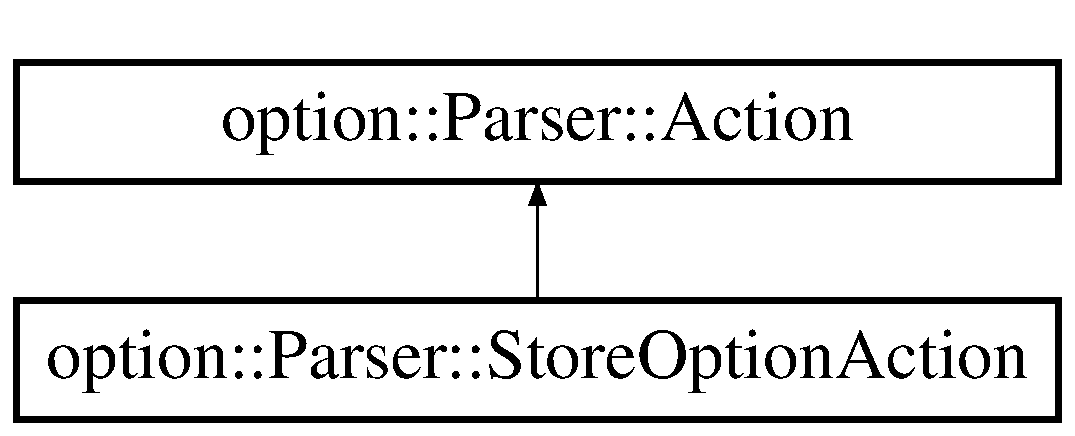
\includegraphics[height=2.000000cm]{classoption_1_1Parser_1_1StoreOptionAction}
\end{center}
\end{figure}
\subsection*{Public Member Functions}
\begin{DoxyCompactItemize}
\item 
\hyperlink{classoption_1_1Parser_1_1StoreOptionAction_aaa638cdd712202e3e10471d4299f7f9d}{Store\+Option\+Action} (\hyperlink{classoption_1_1Parser}{Parser} \&parser\+\_\+, \hyperlink{classoption_1_1Option}{Option} options\+\_\+\mbox{[}$\,$\mbox{]}, \hyperlink{classoption_1_1Option}{Option} buffer\+\_\+\mbox{[}$\,$\mbox{]}, int bufmax\+\_\+)
\begin{DoxyCompactList}\small\item\em Number of slots in {\ttfamily buffer}. {\ttfamily -\/1} means \char`\"{}large enough\char`\"{}. \end{DoxyCompactList}\item 
bool \hyperlink{classoption_1_1Parser_1_1StoreOptionAction_a8931919fba5516377c202920db2b2f84}{perform} (\hyperlink{classoption_1_1Option}{Option} \&option)
\begin{DoxyCompactList}\small\item\em Called by Parser\+::workhorse() for each \hyperlink{classoption_1_1Option}{Option} that has been successfully parsed (including unknown options if they have a \hyperlink{structoption_1_1Descriptor}{Descriptor} whose \hyperlink{structoption_1_1Descriptor_aa5d675dba0214a4abd73007ff163cc67}{Descriptor\+::check\+\_\+arg} does not return \hyperlink{namespaceoption_aee8c76a07877335762631491e7a5a1a9a9528e32563b795bd2930b12d0a5e382d}{A\+R\+G\+\_\+\+I\+L\+L\+E\+G\+AL}. \end{DoxyCompactList}\item 
bool \hyperlink{classoption_1_1Parser_1_1StoreOptionAction_a617f675ef50a72ae36ce91f065bc8441}{finished} (int numargs, const char $\ast$$\ast$args)
\begin{DoxyCompactList}\small\item\em Called by Parser\+::workhorse() after finishing the parse. \end{DoxyCompactList}\end{DoxyCompactItemize}


\subsection{Constructor \& Destructor Documentation}
\mbox{\Hypertarget{classoption_1_1Parser_1_1StoreOptionAction_aaa638cdd712202e3e10471d4299f7f9d}\label{classoption_1_1Parser_1_1StoreOptionAction_aaa638cdd712202e3e10471d4299f7f9d}} 
\index{option\+::\+Parser\+::\+Store\+Option\+Action@{option\+::\+Parser\+::\+Store\+Option\+Action}!Store\+Option\+Action@{Store\+Option\+Action}}
\index{Store\+Option\+Action@{Store\+Option\+Action}!option\+::\+Parser\+::\+Store\+Option\+Action@{option\+::\+Parser\+::\+Store\+Option\+Action}}
\subsubsection{\texorpdfstring{Store\+Option\+Action()}{StoreOptionAction()}}
{\footnotesize\ttfamily option\+::\+Parser\+::\+Store\+Option\+Action\+::\+Store\+Option\+Action (\begin{DoxyParamCaption}\item[{\hyperlink{classoption_1_1Parser}{Parser} \&}]{parser\+\_\+,  }\item[{\hyperlink{classoption_1_1Option}{Option}}]{options\+\_\+\mbox{[}$\,$\mbox{]},  }\item[{\hyperlink{classoption_1_1Option}{Option}}]{buffer\+\_\+\mbox{[}$\,$\mbox{]},  }\item[{int}]{bufmax\+\_\+ }\end{DoxyParamCaption})\hspace{0.3cm}{\ttfamily [inline]}}



Number of slots in {\ttfamily buffer}. {\ttfamily -\/1} means \char`\"{}large enough\char`\"{}. 

Creates a new Store\+Option action. 
\begin{DoxyParams}{Parameters}
{\em parser\+\_\+} & the parser whose op\+\_\+count should be updated. \\
\hline
{\em options\+\_\+} & each \hyperlink{classoption_1_1Option}{Option} {\ttfamily o} is chained into the linked list {\ttfamily options\+\_\+}\mbox{[}o.\+desc-\/$>$index\mbox{]} \\
\hline
{\em buffer\+\_\+} & each \hyperlink{classoption_1_1Option}{Option} is appended to this array as long as there\textquotesingle{}s a free slot. \\
\hline
{\em bufmax\+\_\+} & number of slots in {\ttfamily buffer\+\_\+}. {\ttfamily -\/1} means \char`\"{}large enough\char`\"{}. \\
\hline
\end{DoxyParams}


\subsection{Member Function Documentation}
\mbox{\Hypertarget{classoption_1_1Parser_1_1StoreOptionAction_a617f675ef50a72ae36ce91f065bc8441}\label{classoption_1_1Parser_1_1StoreOptionAction_a617f675ef50a72ae36ce91f065bc8441}} 
\index{option\+::\+Parser\+::\+Store\+Option\+Action@{option\+::\+Parser\+::\+Store\+Option\+Action}!finished@{finished}}
\index{finished@{finished}!option\+::\+Parser\+::\+Store\+Option\+Action@{option\+::\+Parser\+::\+Store\+Option\+Action}}
\subsubsection{\texorpdfstring{finished()}{finished()}}
{\footnotesize\ttfamily bool option\+::\+Parser\+::\+Store\+Option\+Action\+::finished (\begin{DoxyParamCaption}\item[{int}]{numargs,  }\item[{const char $\ast$$\ast$}]{args }\end{DoxyParamCaption})\hspace{0.3cm}{\ttfamily [inline]}, {\ttfamily [virtual]}}



Called by Parser\+::workhorse() after finishing the parse. 


\begin{DoxyParams}{Parameters}
{\em numargs} & the number of non-\/option arguments remaining \\
\hline
{\em args} & pointer to the first remaining non-\/option argument (if numargs $>$ 0).\\
\hline
\end{DoxyParams}
\begin{DoxyReturn}{Returns}
{\ttfamily false} iff a fatal error has occurred. 
\end{DoxyReturn}


Reimplemented from \hyperlink{structoption_1_1Parser_1_1Action_a3ec558b51e34d33d116f14587289e032}{option\+::\+Parser\+::\+Action}.

\mbox{\Hypertarget{classoption_1_1Parser_1_1StoreOptionAction_a8931919fba5516377c202920db2b2f84}\label{classoption_1_1Parser_1_1StoreOptionAction_a8931919fba5516377c202920db2b2f84}} 
\index{option\+::\+Parser\+::\+Store\+Option\+Action@{option\+::\+Parser\+::\+Store\+Option\+Action}!perform@{perform}}
\index{perform@{perform}!option\+::\+Parser\+::\+Store\+Option\+Action@{option\+::\+Parser\+::\+Store\+Option\+Action}}
\subsubsection{\texorpdfstring{perform()}{perform()}}
{\footnotesize\ttfamily bool option\+::\+Parser\+::\+Store\+Option\+Action\+::perform (\begin{DoxyParamCaption}\item[{\hyperlink{classoption_1_1Option}{Option} \&}]{ }\end{DoxyParamCaption})\hspace{0.3cm}{\ttfamily [inline]}, {\ttfamily [virtual]}}



Called by Parser\+::workhorse() for each \hyperlink{classoption_1_1Option}{Option} that has been successfully parsed (including unknown options if they have a \hyperlink{structoption_1_1Descriptor}{Descriptor} whose \hyperlink{structoption_1_1Descriptor_aa5d675dba0214a4abd73007ff163cc67}{Descriptor\+::check\+\_\+arg} does not return \hyperlink{namespaceoption_aee8c76a07877335762631491e7a5a1a9a9528e32563b795bd2930b12d0a5e382d}{A\+R\+G\+\_\+\+I\+L\+L\+E\+G\+AL}. 

Returns {\ttfamily false} iff a fatal error has occured and the parse should be aborted. 

Reimplemented from \hyperlink{structoption_1_1Parser_1_1Action_a176b5f783bb35eb015b6d2c09422457d}{option\+::\+Parser\+::\+Action}.



The documentation for this class was generated from the following file\+:\begin{DoxyCompactItemize}
\item 
headers/\hyperlink{optionparser_8hpp}{optionparser.\+hpp}\end{DoxyCompactItemize}

\hypertarget{structoption_1_1PrintUsageImplementation_1_1StreamWriter}{}\section{option\+:\+:Print\+Usage\+Implementation\+:\+:Stream\+Writer$<$ Function, Stream $>$ Struct Template Reference}
\label{structoption_1_1PrintUsageImplementation_1_1StreamWriter}\index{option\+::\+Print\+Usage\+Implementation\+::\+Stream\+Writer$<$ Function, Stream $>$@{option\+::\+Print\+Usage\+Implementation\+::\+Stream\+Writer$<$ Function, Stream $>$}}
Inheritance diagram for option\+:\+:Print\+Usage\+Implementation\+:\+:Stream\+Writer$<$ Function, Stream $>$\+:\begin{figure}[H]
\begin{center}
\leavevmode
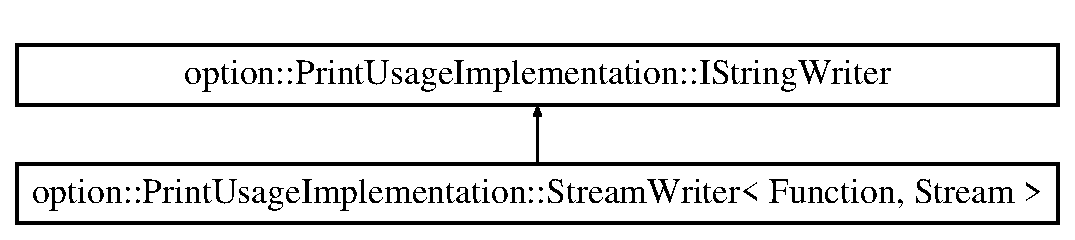
\includegraphics[height=2.000000cm]{structoption_1_1PrintUsageImplementation_1_1StreamWriter}
\end{center}
\end{figure}
\subsection*{Public Member Functions}
\begin{DoxyCompactItemize}
\item 
\mbox{\Hypertarget{structoption_1_1PrintUsageImplementation_1_1StreamWriter_ae39bc6378c22d24a490104b7764c37b7}\label{structoption_1_1PrintUsageImplementation_1_1StreamWriter_ae39bc6378c22d24a490104b7764c37b7}} 
virtual void \hyperlink{structoption_1_1PrintUsageImplementation_1_1StreamWriter_ae39bc6378c22d24a490104b7764c37b7}{operator()} (const char $\ast$str, int size)
\begin{DoxyCompactList}\small\item\em Writes the given number of chars beginning at the given pointer somewhere. \end{DoxyCompactList}\item 
\mbox{\Hypertarget{structoption_1_1PrintUsageImplementation_1_1StreamWriter_aa6ab48848dcbeb9e2cbde5d05ec35005}\label{structoption_1_1PrintUsageImplementation_1_1StreamWriter_aa6ab48848dcbeb9e2cbde5d05ec35005}} 
{\bfseries Stream\+Writer} (Function $\ast$w, Stream $\ast$s)
\end{DoxyCompactItemize}
\subsection*{Public Attributes}
\begin{DoxyCompactItemize}
\item 
\mbox{\Hypertarget{structoption_1_1PrintUsageImplementation_1_1StreamWriter_a6f54abc9a3f7f00206d87a3619713954}\label{structoption_1_1PrintUsageImplementation_1_1StreamWriter_a6f54abc9a3f7f00206d87a3619713954}} 
Function $\ast$ {\bfseries fwrite}
\item 
\mbox{\Hypertarget{structoption_1_1PrintUsageImplementation_1_1StreamWriter_ab4bfd31b1c37376505ccd4230f7f7ad9}\label{structoption_1_1PrintUsageImplementation_1_1StreamWriter_ab4bfd31b1c37376505ccd4230f7f7ad9}} 
Stream $\ast$ {\bfseries stream}
\end{DoxyCompactItemize}


The documentation for this struct was generated from the following file\+:\begin{DoxyCompactItemize}
\item 
headers/\hyperlink{optionparser_8hpp}{optionparser.\+hpp}\end{DoxyCompactItemize}

\hypertarget{structoption_1_1PrintUsageImplementation_1_1SyscallWriter}{}\section{option\+:\+:Print\+Usage\+Implementation\+:\+:Syscall\+Writer$<$ Syscall $>$ Struct Template Reference}
\label{structoption_1_1PrintUsageImplementation_1_1SyscallWriter}\index{option\+::\+Print\+Usage\+Implementation\+::\+Syscall\+Writer$<$ Syscall $>$@{option\+::\+Print\+Usage\+Implementation\+::\+Syscall\+Writer$<$ Syscall $>$}}
Inheritance diagram for option\+:\+:Print\+Usage\+Implementation\+:\+:Syscall\+Writer$<$ Syscall $>$\+:\begin{figure}[H]
\begin{center}
\leavevmode
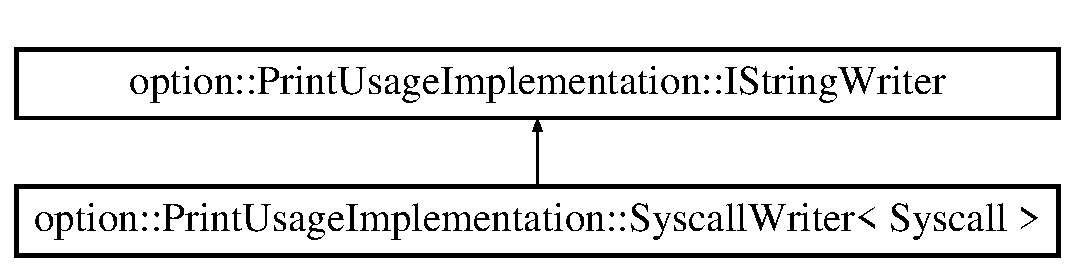
\includegraphics[height=2.000000cm]{structoption_1_1PrintUsageImplementation_1_1SyscallWriter}
\end{center}
\end{figure}
\subsection*{Public Member Functions}
\begin{DoxyCompactItemize}
\item 
\mbox{\Hypertarget{structoption_1_1PrintUsageImplementation_1_1SyscallWriter_a61c1c010d9b67affd5f1208f0a3e9cf0}\label{structoption_1_1PrintUsageImplementation_1_1SyscallWriter_a61c1c010d9b67affd5f1208f0a3e9cf0}} 
virtual void \hyperlink{structoption_1_1PrintUsageImplementation_1_1SyscallWriter_a61c1c010d9b67affd5f1208f0a3e9cf0}{operator()} (const char $\ast$str, int size)
\begin{DoxyCompactList}\small\item\em Writes the given number of chars beginning at the given pointer somewhere. \end{DoxyCompactList}\item 
\mbox{\Hypertarget{structoption_1_1PrintUsageImplementation_1_1SyscallWriter_ae4f8677dbd79b0a9238368e28014701a}\label{structoption_1_1PrintUsageImplementation_1_1SyscallWriter_ae4f8677dbd79b0a9238368e28014701a}} 
{\bfseries Syscall\+Writer} (Syscall $\ast$w, int f)
\end{DoxyCompactItemize}
\subsection*{Public Attributes}
\begin{DoxyCompactItemize}
\item 
\mbox{\Hypertarget{structoption_1_1PrintUsageImplementation_1_1SyscallWriter_adc72b04cd74c69d0219b8b26589b8e5e}\label{structoption_1_1PrintUsageImplementation_1_1SyscallWriter_adc72b04cd74c69d0219b8b26589b8e5e}} 
Syscall $\ast$ {\bfseries write}
\item 
\mbox{\Hypertarget{structoption_1_1PrintUsageImplementation_1_1SyscallWriter_ae79409e3f85f8dbaa7ef87bb8d7fcf8a}\label{structoption_1_1PrintUsageImplementation_1_1SyscallWriter_ae79409e3f85f8dbaa7ef87bb8d7fcf8a}} 
int {\bfseries fd}
\end{DoxyCompactItemize}


The documentation for this struct was generated from the following file\+:\begin{DoxyCompactItemize}
\item 
headers/\hyperlink{optionparser_8hpp}{optionparser.\+hpp}\end{DoxyCompactItemize}

\hypertarget{structoption_1_1PrintUsageImplementation_1_1TemporaryWriter}{}\section{option\+:\+:Print\+Usage\+Implementation\+:\+:Temporary\+Writer$<$ Temporary $>$ Struct Template Reference}
\label{structoption_1_1PrintUsageImplementation_1_1TemporaryWriter}\index{option\+::\+Print\+Usage\+Implementation\+::\+Temporary\+Writer$<$ Temporary $>$@{option\+::\+Print\+Usage\+Implementation\+::\+Temporary\+Writer$<$ Temporary $>$}}
Inheritance diagram for option\+:\+:Print\+Usage\+Implementation\+:\+:Temporary\+Writer$<$ Temporary $>$\+:\begin{figure}[H]
\begin{center}
\leavevmode
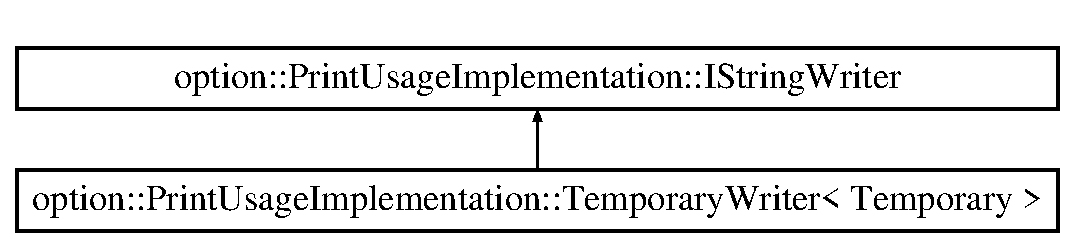
\includegraphics[height=2.000000cm]{structoption_1_1PrintUsageImplementation_1_1TemporaryWriter}
\end{center}
\end{figure}
\subsection*{Public Member Functions}
\begin{DoxyCompactItemize}
\item 
\mbox{\Hypertarget{structoption_1_1PrintUsageImplementation_1_1TemporaryWriter_a674751ddfff63852b36c754878276b02}\label{structoption_1_1PrintUsageImplementation_1_1TemporaryWriter_a674751ddfff63852b36c754878276b02}} 
virtual void \hyperlink{structoption_1_1PrintUsageImplementation_1_1TemporaryWriter_a674751ddfff63852b36c754878276b02}{operator()} (const char $\ast$str, int size)
\begin{DoxyCompactList}\small\item\em Writes the given number of chars beginning at the given pointer somewhere. \end{DoxyCompactList}\item 
\mbox{\Hypertarget{structoption_1_1PrintUsageImplementation_1_1TemporaryWriter_a0c65740b5a897ca2a2465d1c112882a8}\label{structoption_1_1PrintUsageImplementation_1_1TemporaryWriter_a0c65740b5a897ca2a2465d1c112882a8}} 
{\bfseries Temporary\+Writer} (const Temporary \&u)
\end{DoxyCompactItemize}
\subsection*{Public Attributes}
\begin{DoxyCompactItemize}
\item 
\mbox{\Hypertarget{structoption_1_1PrintUsageImplementation_1_1TemporaryWriter_a91d54cfcea7bb4072072506d46cc2cc8}\label{structoption_1_1PrintUsageImplementation_1_1TemporaryWriter_a91d54cfcea7bb4072072506d46cc2cc8}} 
const Temporary \& {\bfseries userstream}
\end{DoxyCompactItemize}


The documentation for this struct was generated from the following file\+:\begin{DoxyCompactItemize}
\item 
headers/\hyperlink{optionparser_8hpp}{optionparser.\+hpp}\end{DoxyCompactItemize}

\hypertarget{classVigenere}{}\section{Vigenere Class Reference}
\label{classVigenere}\index{Vigenere@{Vigenere}}
\subsection*{Public Member Functions}
\begin{DoxyCompactItemize}
\item 
\hyperlink{classVigenere_a3196a2902aa64dde58b84c76a4fb351d}{Vigenere} (string)
\item 
string \hyperlink{classVigenere_a5b73ebb7eed8709e608da556ec3633fa}{decrypt} (string)
\item 
string \hyperlink{classVigenere_ae41574ecb94277c69204a8937a061b15}{encrypt} (string)
\item 
void \hyperlink{classVigenere_ac0ee004df7b389284c9aaa90c7dbcf76}{encrypt\+File} (string, string=\char`\"{}crypt.\+vig\char`\"{})
\item 
void \hyperlink{classVigenere_ad5a357194e5b113037f56adc0602f0b3}{decrypt\+File} (string, string=\char`\"{}plain.\+txt\char`\"{})
\end{DoxyCompactItemize}


\subsection{Constructor \& Destructor Documentation}
\mbox{\Hypertarget{classVigenere_a3196a2902aa64dde58b84c76a4fb351d}\label{classVigenere_a3196a2902aa64dde58b84c76a4fb351d}} 
\index{Vigenere@{Vigenere}!Vigenere@{Vigenere}}
\index{Vigenere@{Vigenere}!Vigenere@{Vigenere}}
\subsubsection{\texorpdfstring{Vigenere()}{Vigenere()}}
{\footnotesize\ttfamily Vigenere\+::\+Vigenere (\begin{DoxyParamCaption}\item[{string}]{key }\end{DoxyParamCaption})}

Constructor to create an en/decrypting object


\begin{DoxyParams}{Parameters}
{\em key} & string to use as a key \\
\hline
\end{DoxyParams}


\subsection{Member Function Documentation}
\mbox{\Hypertarget{classVigenere_a5b73ebb7eed8709e608da556ec3633fa}\label{classVigenere_a5b73ebb7eed8709e608da556ec3633fa}} 
\index{Vigenere@{Vigenere}!decrypt@{decrypt}}
\index{decrypt@{decrypt}!Vigenere@{Vigenere}}
\subsubsection{\texorpdfstring{decrypt()}{decrypt()}}
{\footnotesize\ttfamily string Vigenere\+::decrypt (\begin{DoxyParamCaption}\item[{string}]{text }\end{DoxyParamCaption})}

Currently cannot recover any non a-\/z$\vert$\+A-\/Z and forces to a single case


\begin{DoxyParams}{Parameters}
{\em text} & decrypts a cipher string \\
\hline
\end{DoxyParams}
\begin{DoxyReturn}{Returns}
decrypted text 
\end{DoxyReturn}
\mbox{\Hypertarget{classVigenere_ad5a357194e5b113037f56adc0602f0b3}\label{classVigenere_ad5a357194e5b113037f56adc0602f0b3}} 
\index{Vigenere@{Vigenere}!decrypt\+File@{decrypt\+File}}
\index{decrypt\+File@{decrypt\+File}!Vigenere@{Vigenere}}
\subsubsection{\texorpdfstring{decrypt\+File()}{decryptFile()}}
{\footnotesize\ttfamily void Vigenere\+::decrypt\+File (\begin{DoxyParamCaption}\item[{string}]{file,  }\item[{string}]{out = {\ttfamily \char`\"{}plain.txt\char`\"{}} }\end{DoxyParamCaption})}

performs decryption on a single text file. All non a-\/z$\vert$\+A-\/Z is stripped.

key is reset so later calls are not affected by earlier calls.


\begin{DoxyParams}{Parameters}
{\em file} & Name of file to decrypt \\
\hline
{\em out} & optional name of output file \\
\hline
\end{DoxyParams}
\mbox{\Hypertarget{classVigenere_ae41574ecb94277c69204a8937a061b15}\label{classVigenere_ae41574ecb94277c69204a8937a061b15}} 
\index{Vigenere@{Vigenere}!encrypt@{encrypt}}
\index{encrypt@{encrypt}!Vigenere@{Vigenere}}
\subsubsection{\texorpdfstring{encrypt()}{encrypt()}}
{\footnotesize\ttfamily string Vigenere\+::encrypt (\begin{DoxyParamCaption}\item[{string}]{text }\end{DoxyParamCaption})}

Currently strips any non a-\/z$\vert$\+A-\/Z and forces to a single case


\begin{DoxyParams}{Parameters}
{\em text} & encrypts a plaintext string \\
\hline
\end{DoxyParams}
\begin{DoxyReturn}{Returns}
encrypted text 
\end{DoxyReturn}
\mbox{\Hypertarget{classVigenere_ac0ee004df7b389284c9aaa90c7dbcf76}\label{classVigenere_ac0ee004df7b389284c9aaa90c7dbcf76}} 
\index{Vigenere@{Vigenere}!encrypt\+File@{encrypt\+File}}
\index{encrypt\+File@{encrypt\+File}!Vigenere@{Vigenere}}
\subsubsection{\texorpdfstring{encrypt\+File()}{encryptFile()}}
{\footnotesize\ttfamily void Vigenere\+::encrypt\+File (\begin{DoxyParamCaption}\item[{string}]{file,  }\item[{string}]{out = {\ttfamily \char`\"{}crypt.vig\char`\"{}} }\end{DoxyParamCaption})}

performs encryption on a single text file. All non a-\/z$\vert$\+A-\/Z is stripped.

key is reset so later calls are not affected by earlier calls.


\begin{DoxyParams}{Parameters}
{\em file} & Name of file to encrypt \\
\hline
{\em out} & optional name of output file \\
\hline
\end{DoxyParams}


The documentation for this class was generated from the following files\+:\begin{DoxyCompactItemize}
\item 
headers/\hyperlink{Vigenere_8hpp}{Vigenere.\+hpp}\item 
sources/\hyperlink{Vigenere_8cpp}{Vigenere.\+cpp}\end{DoxyCompactItemize}

\chapter{File Documentation}
\hypertarget{FileManager_8hpp}{}\section{headers/\+File\+Manager.hpp File Reference}
\label{FileManager_8hpp}\index{headers/\+File\+Manager.\+hpp@{headers/\+File\+Manager.\+hpp}}
\subsection*{Classes}
\begin{DoxyCompactItemize}
\item 
class \hyperlink{classFileManager}{File\+Manager}
\end{DoxyCompactItemize}


\subsection{Detailed Description}
\begin{DoxyVersion}{Version}
0.\+1 
\end{DoxyVersion}
\begin{DoxyAuthor}{Author}
Leo Sleet
\end{DoxyAuthor}
File I/O utilities

\begin{DoxyVersion}{Version}
0.\+1 
\end{DoxyVersion}
\begin{DoxyAuthor}{Author}
Leo Sleet
\end{DoxyAuthor}
Header for File\+Manager.\+cpp 
\hypertarget{Frequency_8hpp}{}\section{headers/\+Frequency.hpp File Reference}
\label{Frequency_8hpp}\index{headers/\+Frequency.\+hpp@{headers/\+Frequency.\+hpp}}
\subsection*{Classes}
\begin{DoxyCompactItemize}
\item 
class \hyperlink{classFrequency}{Frequency}
\item 
class \hyperlink{classRelFrequency}{Rel\+Frequency}
\end{DoxyCompactItemize}


\subsection{Detailed Description}
\begin{DoxyVersion}{Version}
0.\+1 
\end{DoxyVersion}
\begin{DoxyAuthor}{Author}
Leo Sleet
\end{DoxyAuthor}
Header for \hyperlink{Frequency_8cpp}{Frequency.\+cpp} 
\hypertarget{KeyAnalyser_8hpp}{}\section{headers/\+Key\+Analyser.hpp File Reference}
\label{KeyAnalyser_8hpp}\index{headers/\+Key\+Analyser.\+hpp@{headers/\+Key\+Analyser.\+hpp}}
{\ttfamily \#include $<$set$>$}\newline
{\ttfamily \#include $<$thread$>$}\newline
\subsection*{Classes}
\begin{DoxyCompactItemize}
\item 
class \hyperlink{classFriedmann}{Friedmann}
\item 
class \hyperlink{classKasiski}{Kasiski}
\item 
class \hyperlink{classKerckhoff}{Kerckhoff}
\item 
class \hyperlink{classKeyEliminator}{Key\+Eliminator}
\item 
class \hyperlink{classKeyBrute}{Key\+Brute}
\end{DoxyCompactItemize}


\subsection{Detailed Description}
\begin{DoxyVersion}{Version}
0.\+1 
\end{DoxyVersion}
\begin{DoxyAuthor}{Author}
Leo Sleet
\end{DoxyAuthor}
Header for \hyperlink{KeyAnalyser_8cpp}{Key\+Analyser.\+cpp} 
\hypertarget{Language_8hpp}{}\section{headers/\+Language.hpp File Reference}
\label{Language_8hpp}\index{headers/\+Language.\+hpp@{headers/\+Language.\+hpp}}
{\ttfamily \#include $<$Frequency.\+hpp$>$}\newline
\subsection*{Classes}
\begin{DoxyCompactItemize}
\item 
class \hyperlink{classLanguage}{Language}
\item 
class \hyperlink{classEnglish}{English}
\end{DoxyCompactItemize}


\subsection{Detailed Description}
\begin{DoxyVersion}{Version}
0.\+1 
\end{DoxyVersion}
\begin{DoxyAuthor}{Author}
Leo Sleet
\end{DoxyAuthor}
Header for Language.\+cpp 
\hypertarget{optionparser_8hpp}{}\section{headers/optionparser.hpp File Reference}
\label{optionparser_8hpp}\index{headers/optionparser.\+hpp@{headers/optionparser.\+hpp}}


This is the only file required to use The Lean Mean C++ Option Parser. Just \#include it and you\textquotesingle{}re set.  


\subsection*{Classes}
\begin{DoxyCompactItemize}
\item 
struct \hyperlink{structoption_1_1Descriptor}{option\+::\+Descriptor}
\begin{DoxyCompactList}\small\item\em Describes an option, its help text (usage) and how it should be parsed. \end{DoxyCompactList}\item 
class \hyperlink{classoption_1_1Option}{option\+::\+Option}
\begin{DoxyCompactList}\small\item\em A parsed option from the command line together with its argument if it has one. \end{DoxyCompactList}\item 
struct \hyperlink{structoption_1_1Arg}{option\+::\+Arg}
\begin{DoxyCompactList}\small\item\em Functions for checking the validity of option arguments. \end{DoxyCompactList}\item 
struct \hyperlink{structoption_1_1Stats}{option\+::\+Stats}
\begin{DoxyCompactList}\small\item\em Determines the minimum lengths of the buffer and options arrays used for \hyperlink{classoption_1_1Parser}{Parser}. \end{DoxyCompactList}\item 
class \hyperlink{classoption_1_1Parser}{option\+::\+Parser}
\begin{DoxyCompactList}\small\item\em Checks argument vectors for validity and parses them into data structures that are easier to work with. \end{DoxyCompactList}\item 
struct \hyperlink{structoption_1_1Parser_1_1Action}{option\+::\+Parser\+::\+Action}
\item 
class \hyperlink{classoption_1_1Stats_1_1CountOptionsAction}{option\+::\+Stats\+::\+Count\+Options\+Action}
\item 
class \hyperlink{classoption_1_1Parser_1_1StoreOptionAction}{option\+::\+Parser\+::\+Store\+Option\+Action}
\item 
struct \hyperlink{structoption_1_1PrintUsageImplementation}{option\+::\+Print\+Usage\+Implementation}
\item 
struct \hyperlink{structoption_1_1PrintUsageImplementation_1_1IStringWriter}{option\+::\+Print\+Usage\+Implementation\+::\+I\+String\+Writer}
\item 
struct \hyperlink{structoption_1_1PrintUsageImplementation_1_1FunctionWriter}{option\+::\+Print\+Usage\+Implementation\+::\+Function\+Writer$<$ Function $>$}
\item 
struct \hyperlink{structoption_1_1PrintUsageImplementation_1_1OStreamWriter}{option\+::\+Print\+Usage\+Implementation\+::\+O\+Stream\+Writer$<$ O\+Stream $>$}
\item 
struct \hyperlink{structoption_1_1PrintUsageImplementation_1_1TemporaryWriter}{option\+::\+Print\+Usage\+Implementation\+::\+Temporary\+Writer$<$ Temporary $>$}
\item 
struct \hyperlink{structoption_1_1PrintUsageImplementation_1_1SyscallWriter}{option\+::\+Print\+Usage\+Implementation\+::\+Syscall\+Writer$<$ Syscall $>$}
\item 
struct \hyperlink{structoption_1_1PrintUsageImplementation_1_1StreamWriter}{option\+::\+Print\+Usage\+Implementation\+::\+Stream\+Writer$<$ Function, Stream $>$}
\item 
class \hyperlink{classoption_1_1PrintUsageImplementation_1_1LinePartIterator}{option\+::\+Print\+Usage\+Implementation\+::\+Line\+Part\+Iterator}
\item 
class \hyperlink{classoption_1_1PrintUsageImplementation_1_1LineWrapper}{option\+::\+Print\+Usage\+Implementation\+::\+Line\+Wrapper}
\end{DoxyCompactItemize}
\subsection*{Namespaces}
\begin{DoxyCompactItemize}
\item 
 \hyperlink{namespaceoption}{option}
\begin{DoxyCompactList}\small\item\em The namespace of The Lean Mean C++ \hyperlink{classoption_1_1Option}{Option} \hyperlink{classoption_1_1Parser}{Parser}. \end{DoxyCompactList}\end{DoxyCompactItemize}
\subsection*{Typedefs}
\begin{DoxyCompactItemize}
\item 
typedef Arg\+Status($\ast$ \hyperlink{namespaceoption_a4cdf403efae65e18bf850e2001b12a2a}{option\+::\+Check\+Arg}) (const Option \&option, bool msg)
\begin{DoxyCompactList}\small\item\em Signature of functions that check if an argument is valid for a certain type of option. \end{DoxyCompactList}\end{DoxyCompactItemize}
\subsection*{Enumerations}
\begin{DoxyCompactItemize}
\item 
enum \hyperlink{namespaceoption_aee8c76a07877335762631491e7a5a1a9}{option\+::\+Arg\+Status} \{ \hyperlink{namespaceoption_aee8c76a07877335762631491e7a5a1a9a353903b042e8eb0aa2f60c0043a58a7e}{option\+::\+A\+R\+G\+\_\+\+N\+O\+NE}, 
\hyperlink{namespaceoption_aee8c76a07877335762631491e7a5a1a9a445e08cb1747e5a22929e7ef2da43b55}{option\+::\+A\+R\+G\+\_\+\+OK}, 
\hyperlink{namespaceoption_aee8c76a07877335762631491e7a5a1a9a83e0837c79c957525918111d33cab3a9}{option\+::\+A\+R\+G\+\_\+\+I\+G\+N\+O\+RE}, 
\hyperlink{namespaceoption_aee8c76a07877335762631491e7a5a1a9a9528e32563b795bd2930b12d0a5e382d}{option\+::\+A\+R\+G\+\_\+\+I\+L\+L\+E\+G\+AL}
 \}\begin{DoxyCompactList}\small\item\em Possible results when checking if an argument is valid for a certain option. \end{DoxyCompactList}
\end{DoxyCompactItemize}
\subsection*{Functions}
\begin{DoxyCompactItemize}
\item 
{\footnotesize template$<$typename O\+Stream $>$ }\\void \hyperlink{namespaceoption_afc8bb7e040a98a0b33ff1ce9da1be0d1}{option\+::print\+Usage} (O\+Stream \&prn, const Descriptor usage\mbox{[}$\,$\mbox{]}, int width=80, int last\+\_\+column\+\_\+min\+\_\+percent=50, int last\+\_\+column\+\_\+own\+\_\+line\+\_\+max\+\_\+percent=75)
\begin{DoxyCompactList}\small\item\em Outputs a nicely formatted usage string with support for multi-\/column formatting and line-\/wrapping. \end{DoxyCompactList}\item 
\mbox{\Hypertarget{namespaceoption_a846de0735717c8402b76d14f0a7a4430}\label{namespaceoption_a846de0735717c8402b76d14f0a7a4430}} 
{\footnotesize template$<$typename Function $>$ }\\void {\bfseries option\+::print\+Usage} (Function $\ast$prn, const Descriptor usage\mbox{[}$\,$\mbox{]}, int width=80, int last\+\_\+column\+\_\+min\+\_\+percent=50, int last\+\_\+column\+\_\+own\+\_\+line\+\_\+max\+\_\+percent=75)
\item 
\mbox{\Hypertarget{namespaceoption_a86e12a019c4da81e5031901af9c800cc}\label{namespaceoption_a86e12a019c4da81e5031901af9c800cc}} 
{\footnotesize template$<$typename Temporary $>$ }\\void {\bfseries option\+::print\+Usage} (const Temporary \&prn, const Descriptor usage\mbox{[}$\,$\mbox{]}, int width=80, int last\+\_\+column\+\_\+min\+\_\+percent=50, int last\+\_\+column\+\_\+own\+\_\+line\+\_\+max\+\_\+percent=75)
\item 
\mbox{\Hypertarget{namespaceoption_a84764f72d05ba8480143043e3d56ad6a}\label{namespaceoption_a84764f72d05ba8480143043e3d56ad6a}} 
{\footnotesize template$<$typename Syscall $>$ }\\void {\bfseries option\+::print\+Usage} (Syscall $\ast$prn, int fd, const Descriptor usage\mbox{[}$\,$\mbox{]}, int width=80, int last\+\_\+column\+\_\+min\+\_\+percent=50, int last\+\_\+column\+\_\+own\+\_\+line\+\_\+max\+\_\+percent=75)
\item 
\mbox{\Hypertarget{namespaceoption_a27bfa29dc37bb1bfc5e0b891509e5881}\label{namespaceoption_a27bfa29dc37bb1bfc5e0b891509e5881}} 
{\footnotesize template$<$typename Function , typename Stream $>$ }\\void {\bfseries option\+::print\+Usage} (Function $\ast$prn, Stream $\ast$stream, const Descriptor usage\mbox{[}$\,$\mbox{]}, int width=80, int last\+\_\+column\+\_\+min\+\_\+percent=50, int last\+\_\+column\+\_\+own\+\_\+line\+\_\+max\+\_\+percent=75)
\end{DoxyCompactItemize}


\subsection{Detailed Description}
This is the only file required to use The Lean Mean C++ Option Parser. Just \#include it and you\textquotesingle{}re set. 

The Lean Mean C++ Option Parser handles the program\textquotesingle{}s command line arguments (argc, argv). It supports the short and long option formats of getopt(), getopt\+\_\+long() and getopt\+\_\+long\+\_\+only() but has a more convenient interface. The following features set it apart from other option parsers\+:

\begin{DoxyParagraph}{Highlights\+:}

\begin{DoxyItemize}
\item It is a header-\/only library. Just {\ttfamily \#include \char`\"{}optionparser.\+h\char`\"{}} and you\textquotesingle{}re set. 
\item It is freestanding. There are no dependencies whatsoever, not even the C or C++ standard library. 
\item It has a usage message formatter that supports column alignment and line wrapping. This aids localization because it adapts to translated strings that are shorter or longer (even if they contain Asian wide characters). 
\item Unlike getopt() and derivatives it doesn\textquotesingle{}t force you to loop through options sequentially. Instead you can access options directly like this\+: 
\begin{DoxyItemize}
\item Test for presence of a switch in the argument vector\+: 
\begin{DoxyCode}
\textcolor{keywordflow}{if} ( options[QUIET] ) ... 
\end{DoxyCode}
 
\item Evaluate --enable-\/foo/--disable-\/foo pair where the last one used wins\+: 
\begin{DoxyCode}
\textcolor{keywordflow}{if} ( options[FOO].last()->type() == DISABLE ) ... 
\end{DoxyCode}
 
\item Cumulative option (-\/v verbose, -\/vv more verbose, -\/vvv even more verbose)\+: 
\begin{DoxyCode}
\textcolor{keywordtype}{int} verbosity = options[VERBOSE].\hyperlink{classoption_1_1Option_a8a632dcd89af60fe0806deb756c08f14}{count}(); 
\end{DoxyCode}
 
\item Iterate over all --file=$<$fname$>$ arguments\+: 
\begin{DoxyCode}
\textcolor{keywordflow}{for} (Option* opt = options[FILE]; opt; opt = opt->\hyperlink{classoption_1_1Option_a59ae9aed505f4d410633bb36478a32be}{next}())
 fname = opt->arg; ... 
\end{DoxyCode}
 
\item If you really want to, you can still process all arguments in order\+: 
\begin{DoxyCode}
\textcolor{keywordflow}{for} (\textcolor{keywordtype}{int} i = 0; i < p.optionsCount(); ++i) \{
  Option& opt = buffer[i];
  \textcolor{keywordflow}{switch}(opt.index()) \{
    \textcolor{keywordflow}{case} HELP:    ...
    \textcolor{keywordflow}{case} VERBOSE: ...
    \textcolor{keywordflow}{case} FILE:    fname = opt.arg; ...
    \textcolor{keywordflow}{case} UNKNOWN: ...
\end{DoxyCode}
 
\end{DoxyItemize}
\end{DoxyItemize}~\newline
Despite these features the code size remains tiny. It is smaller than \href{http://uclibc.org}{\tt u\+Clibc}\textquotesingle{}s G\+NU getopt() and just a couple 100 bytes larger than u\+Clibc\textquotesingle{}s S\+U\+Sv3 getopt(). ~\newline
(This does not include the usage formatter, of course. But you don\textquotesingle{}t have to use that.)
\end{DoxyParagraph}
\begin{DoxyParagraph}{Download\+:}
Tarball with examples and test programs\+: \href{http://sourceforge.net/projects/optionparser/files/optionparser-1.4.tar.gz/download}{\tt optionparser-\/1.\+4.\+tar.\+gz} ~\newline
Just the header (this is all you really need)\+: \href{http://optionparser.sourceforge.net/optionparser.h}{\tt optionparser.\+h}
\end{DoxyParagraph}
\begin{DoxyParagraph}{Changelog\+:}
{\bfseries Version 1.\+4\+:} Fixed 2 print\+Usage() bugs that messed up output with small C\+O\+L\+U\+M\+NS values ~\newline
{\bfseries Version 1.\+3\+:} Compatible with Microsoft Visual C++. ~\newline
{\bfseries Version 1.\+2\+:} Added \hyperlink{classoption_1_1Option_a3aa2957b19ad5815873441b415d56050}{Option\+:\+:namelen} and removed the extraction of short option characters into a special buffer. ~\newline
 Changed \hyperlink{structoption_1_1Arg_aadb5316ecbc9eb0a7f0019d14bf35ad0}{Arg\+:\+:Optional} to accept arguments if they are attached rather than separate. This is what G\+NU getopt() does and how P\+O\+S\+IX recommends utilities should interpret their arguments.~\newline
{\bfseries Version 1.\+1\+:} Optional mode with argument reordering as done by G\+NU getopt(), so that options and non-\/options can be mixed. See \hyperlink{classoption_1_1Parser_a6e0b5778d1cfbd6cd51240e74d01e138}{Parser\+:\+:parse()}.
\end{DoxyParagraph}
\begin{DoxyParagraph}{Feedback\+:}
Send questions, bug reports, feature requests etc. to\+: {\ttfamily {\bfseries optionparser-\/feedback~(a)~lists.\+sourceforge.\+net}} 
\end{DoxyParagraph}
\begin{DoxyParagraph}{Example program\+:}
(Note\+: {\ttfamily option\+:}\+:$\ast$ identifiers are links that take you to their documentation.) 
\begin{DoxyCode}
\textcolor{preprocessor}{#error EXAMPLE SHORTENED FOR READABILITY. BETTER EXAMPLES ARE IN THE .TAR.GZ!}
\textcolor{preprocessor}{#include <iostream>}
\textcolor{preprocessor}{#include "optionparser.h"}

\textcolor{keyword}{enum}  optionIndex \{ UNKNOWN, HELP, PLUS \};
\textcolor{keyword}{const} \hyperlink{structoption_1_1Descriptor}{option::Descriptor} usage[] =
\{
 \{UNKNOWN, 0,\textcolor{stringliteral}{""} , \textcolor{stringliteral}{""}    ,\hyperlink{structoption_1_1Arg_a7fc01987899c91c6b6a1be5711a46e22}{option::Arg::None}, \textcolor{stringliteral}{"USAGE: example [options]\(\backslash\)n\(\backslash\)n"}
                                            \textcolor{stringliteral}{"Options:"} \},
 \{HELP,    0,\textcolor{stringliteral}{""} , \textcolor{stringliteral}{"help"},\hyperlink{structoption_1_1Arg_a7fc01987899c91c6b6a1be5711a46e22}{option::Arg::None}, \textcolor{stringliteral}{"  --help  \(\backslash\)tPrint usage and exit."} \},
 \{PLUS,    0,\textcolor{stringliteral}{"p"}, \textcolor{stringliteral}{"plus"},\hyperlink{structoption_1_1Arg_a7fc01987899c91c6b6a1be5711a46e22}{option::Arg::None}, \textcolor{stringliteral}{"  --plus, -p  \(\backslash\)tIncrement count."} \},
 \{UNKNOWN, 0,\textcolor{stringliteral}{""} ,  \textcolor{stringliteral}{""}   ,\hyperlink{structoption_1_1Arg_a7fc01987899c91c6b6a1be5711a46e22}{option::Arg::None}, \textcolor{stringliteral}{"\(\backslash\)nExamples:\(\backslash\)n"}
                                            \textcolor{stringliteral}{"  example --unknown -- --this\_is\_no\_option\(\backslash\)n"}
                                            \textcolor{stringliteral}{"  example -unk --plus -ppp file1 file2\(\backslash\)n"} \},
 \{0,0,0,0,0,0\}
\};

\textcolor{keywordtype}{int} main(\textcolor{keywordtype}{int} argc, \textcolor{keywordtype}{char}* argv[])
\{
  argc-=(argc>0); argv+=(argc>0); \textcolor{comment}{// skip program name argv[0] if present}
  \hyperlink{structoption_1_1Stats}{option::Stats}  stats(usage, argc, argv);
  \hyperlink{classoption_1_1Option}{option::Option} options[stats.options\_max], buffer[stats.buffer\_max];
  \hyperlink{classoption_1_1Parser}{option::Parser} parse(usage, argc, argv, options, buffer);

  \textcolor{keywordflow}{if} (parse.error())
    \textcolor{keywordflow}{return} 1;

  \textcolor{keywordflow}{if} (options[HELP] || argc == 0) \{
    \hyperlink{namespaceoption_afc8bb7e040a98a0b33ff1ce9da1be0d1}{option::printUsage}(std::cout, usage);
    \textcolor{keywordflow}{return} 0;
  \}

  std::cout << \textcolor{stringliteral}{"--plus count: "} <<
    options[PLUS].\hyperlink{classoption_1_1Option_a8a632dcd89af60fe0806deb756c08f14}{count}() << \textcolor{stringliteral}{"\(\backslash\)n"};

  \textcolor{keywordflow}{for} (\hyperlink{classoption_1_1Option}{option::Option}* opt = options[UNKNOWN]; opt; opt = opt->
      \hyperlink{classoption_1_1Option_a59ae9aed505f4d410633bb36478a32be}{next}())
    std::cout << \textcolor{stringliteral}{"Unknown option: "} << opt->name << \textcolor{stringliteral}{"\(\backslash\)n"};

  for (\textcolor{keywordtype}{int} i = 0; i < parse.nonOptionsCount(); ++i)
    std::cout << \textcolor{stringliteral}{"Non-option #"} << i << \textcolor{stringliteral}{": "} << parse.nonOption(i) << \textcolor{stringliteral}{"\(\backslash\)n"};
\}
\end{DoxyCode}

\end{DoxyParagraph}
\begin{DoxyParagraph}{Option syntax\+:}
\begin{DoxyItemize}
\item The Lean Mean C++ Option Parser follows P\+O\+S\+IX {\ttfamily getopt()} conventions and supports G\+N\+U-\/style {\ttfamily getopt\+\_\+long()} long options as well as Perl-\/style single-\/minus long options ({\ttfamily getopt\+\_\+long\+\_\+only()}). \item short options have the format {\ttfamily -\/X} where {\ttfamily X} is any character that fits in a char. \item short options can be grouped, i.\+e. {\ttfamily -\/X -\/Y} is equivalent to {\ttfamily -\/\+XY}. \item a short option may take an argument either separate ({\ttfamily -\/X foo}) or attached ({\ttfamily -\/\+Xfoo}). You can make the parser accept the additional format {\ttfamily -\/X=foo} by registering {\ttfamily X} as a long option (in addition to being a short option) and enabling single-\/minus long options. \item an argument-\/taking short option may be grouped if it is the last in the group, e.\+g. {\ttfamily -\/\+A\+B\+C\+Xfoo} or {\ttfamily  -\/\+A\+B\+CX foo } ({\ttfamily foo} is the argument to the {\ttfamily -\/X} option). \item a lone minus character {\ttfamily \textquotesingle{}-\/\textquotesingle{}} is not treated as an option. It is customarily used where a file name is expected to refer to stdin or stdout. \item long options have the format {\ttfamily --option-\/name}. \item the option-\/name of a long option can be anything and include any characters. Even {\ttfamily =} characters will work, but don\textquotesingle{}t do that. \item \mbox{[}optional\mbox{]} long options may be abbreviated as long as the abbreviation is unambiguous. You can set a minimum length for abbreviations. \item \mbox{[}optional\mbox{]} long options may begin with a single minus. The double minus form is always accepted, too. \item a long option may take an argument either separate ({\ttfamily  --option arg }) or attached ({\ttfamily  --option=arg }). In the attached form the equals sign is mandatory. \item an empty string can be passed as an attached long option argument\+: {\ttfamily  --option-\/name= }. Note the distinction between an empty string as argument and no argument at all. \item an empty string is permitted as separate argument to both long and short options. \item Arguments to both short and long options may start with a {\ttfamily \textquotesingle{}-\/\textquotesingle{}} character. E.\+g. {\ttfamily  -\/\+X-\/X }, {\ttfamily -\/X -\/X} or {\ttfamily  --long-\/X=-\/X }. If {\ttfamily -\/X} and {\ttfamily --long-\/X} take an argument, that argument will be {\ttfamily \char`\"{}-\/\+X\char`\"{}} in all 3 cases. \item If using the built-\/in \hyperlink{structoption_1_1Arg_aadb5316ecbc9eb0a7f0019d14bf35ad0}{Arg\+:\+:Optional}, optional arguments must be attached. \item the special option {\ttfamily --} (i.\+e. without a name) terminates the list of options. Everything that follows is a non-\/option argument, even if it starts with a {\ttfamily \textquotesingle{}-\/\textquotesingle{}} character. The {\ttfamily --} itself will not appear in the parse results. \item the first argument that doesn\textquotesingle{}t start with {\ttfamily \textquotesingle{}-\/\textquotesingle{}} or {\ttfamily \textquotesingle{}--\textquotesingle{}} and does not belong to a preceding argument-\/taking option, will terminate the option list and is the first non-\/option argument. All following command line arguments are treated as non-\/option arguments, even if they start with {\ttfamily \textquotesingle{}-\/\textquotesingle{}} . ~\newline
 N\+O\+TE\+: This behaviour is mandated by P\+O\+S\+IX, but G\+NU getopt() only honours this if it is explicitly requested (e.\+g. by setting P\+O\+S\+I\+X\+L\+Y\+\_\+\+C\+O\+R\+R\+E\+CT). ~\newline
 You can enable the G\+NU behaviour by passing {\ttfamily true} as first argument to e.\+g. \hyperlink{classoption_1_1Parser_a6e0b5778d1cfbd6cd51240e74d01e138}{Parser\+:\+:parse()}. \item Arguments that look like options (i.\+e. {\ttfamily \textquotesingle{}-\/\textquotesingle{}} followed by at least 1 character) but aren\textquotesingle{}t, are N\+OT treated as non-\/option arguments. They are treated as unknown options and are collected into a list of unknown options for error reporting. ~\newline
 This means that in order to pass a first non-\/option argument beginning with the minus character it is required to use the {\ttfamily --} special option, e.\+g. 
\begin{DoxyCode}
program -x -- --strange-filename
\end{DoxyCode}
 In this example, {\ttfamily --strange-\/filename} is a non-\/option argument. If the {\ttfamily --} were omitted, it would be treated as an unknown option. ~\newline
 See \hyperlink{structoption_1_1Descriptor_a470c449dfa894c9bfda2dae026142b4b}{option\+::\+Descriptor\+::longopt} for information on how to collect unknown options. \end{DoxyItemize}

\end{DoxyParagraph}

\hypertarget{PolyCrack_8hpp}{}\section{headers/\+Poly\+Crack.hpp File Reference}
\label{PolyCrack_8hpp}\index{headers/\+Poly\+Crack.\+hpp@{headers/\+Poly\+Crack.\+hpp}}
{\ttfamily \#include $<$cstdlib$>$}\newline
{\ttfamily \#include $<$iostream$>$}\newline
{\ttfamily \#include $<$fstream$>$}\newline
{\ttfamily \#include $<$map$>$}\newline
{\ttfamily \#include $<$string$>$}\newline
{\ttfamily \#include $<$list$>$}\newline
\subsection*{Functions}
\begin{DoxyCompactItemize}
\item 
\mbox{\Hypertarget{PolyCrack_8hpp_a84773f4630d1fd10599003eee72db7f8}\label{PolyCrack_8hpp_a84773f4630d1fd10599003eee72db7f8}} 
string {\bfseries make\+Lower} (string)
\item 
\mbox{\Hypertarget{PolyCrack_8hpp_a44eecd5da4b59be29963056af77f4b8c}\label{PolyCrack_8hpp_a44eecd5da4b59be29963056af77f4b8c}} 
string {\bfseries make\+Upper} (string)
\item 
\mbox{\Hypertarget{PolyCrack_8hpp_aafa533aafb825b8206a0cc5a53da8011}\label{PolyCrack_8hpp_aafa533aafb825b8206a0cc5a53da8011}} 
string {\bfseries clean\+Punc} (string)
\item 
\mbox{\Hypertarget{PolyCrack_8hpp_a4e7e78fb7cb4acead6661206ac2a50fe}\label{PolyCrack_8hpp_a4e7e78fb7cb4acead6661206ac2a50fe}} 
string {\bfseries clean\+Num} (string)
\item 
\mbox{\Hypertarget{PolyCrack_8hpp_aa6bdb7a84cefca7feb6d71f4c621a931}\label{PolyCrack_8hpp_aa6bdb7a84cefca7feb6d71f4c621a931}} 
string {\bfseries clean\+White} (string)
\item 
\mbox{\Hypertarget{PolyCrack_8hpp_a4f31d20121f98d4e6de5ff87f640ea0e}\label{PolyCrack_8hpp_a4f31d20121f98d4e6de5ff87f640ea0e}} 
string {\bfseries pure\+String} (string)
\item 
\mbox{\Hypertarget{PolyCrack_8hpp_a8782a0ffaf28e05300878ec90d58ddd6}\label{PolyCrack_8hpp_a8782a0ffaf28e05300878ec90d58ddd6}} 
string {\bfseries clean\+Quotes} (string)
\item 
\mbox{\Hypertarget{PolyCrack_8hpp_a57900e65109780bcd40b13859f44273a}\label{PolyCrack_8hpp_a57900e65109780bcd40b13859f44273a}} 
string {\bfseries make\+A\+S\+C\+II} (string)
\end{DoxyCompactItemize}


\subsection{Detailed Description}
\begin{DoxyVersion}{Version}
0.\+1 
\end{DoxyVersion}
\begin{DoxyAuthor}{Author}
Leo Sleet 
\end{DoxyAuthor}

\hypertarget{Vigenere_8hpp}{}\section{headers/\+Vigenere.hpp File Reference}
\label{Vigenere_8hpp}\index{headers/\+Vigenere.\+hpp@{headers/\+Vigenere.\+hpp}}
\subsection*{Classes}
\begin{DoxyCompactItemize}
\item 
class \hyperlink{classVigenere}{Vigenere}
\end{DoxyCompactItemize}


\subsection{Detailed Description}
\begin{DoxyVersion}{Version}
0.\+1 
\end{DoxyVersion}
\begin{DoxyAuthor}{Author}
Leo Sleet
\end{DoxyAuthor}
Header for \hyperlink{Vigenere_8cpp}{Vigenere.\+cpp} 
\hypertarget{Frequency_8cpp}{}\section{sources/\+Frequency.cpp File Reference}
\label{Frequency_8cpp}\index{sources/\+Frequency.\+cpp@{sources/\+Frequency.\+cpp}}
{\ttfamily \#include $<$Poly\+Crack.\+hpp$>$}\newline
{\ttfamily \#include $<$Frequency.\+hpp$>$}\newline
{\ttfamily \#include $<$File\+Manager.\+hpp$>$}\newline
{\ttfamily \#include $<$functional$>$}\newline
{\ttfamily \#include $<$algorithm$>$}\newline


\subsection{Detailed Description}
\begin{DoxyVersion}{Version}
0.\+1 
\end{DoxyVersion}
\begin{DoxyAuthor}{Author}
Leo Sleet
\end{DoxyAuthor}
A wrapper defining the absolute or relative frequencies of an abstract body of text. 
\hypertarget{KeyAnalyser_8cpp}{}\section{sources/\+Key\+Analyser.cpp File Reference}
\label{KeyAnalyser_8cpp}\index{sources/\+Key\+Analyser.\+cpp@{sources/\+Key\+Analyser.\+cpp}}
{\ttfamily \#include $<$Poly\+Crack.\+hpp$>$}\newline
{\ttfamily \#include $<$Frequency.\+hpp$>$}\newline
{\ttfamily \#include $<$File\+Manager.\+hpp$>$}\newline
{\ttfamily \#include $<$Key\+Analyser.\+hpp$>$}\newline
{\ttfamily \#include $<$set$>$}\newline
{\ttfamily \#include $<$map$>$}\newline
{\ttfamily \#include $<$cmath$>$}\newline
\subsection*{Macros}
\begin{DoxyCompactItemize}
\item 
\mbox{\Hypertarget{KeyAnalyser_8cpp_aa4729260b732666338dee7d841aa12f3}\label{KeyAnalyser_8cpp_aa4729260b732666338dee7d841aa12f3}} 
\#define {\bfseries KP}~0.\+067
\item 
\mbox{\Hypertarget{KeyAnalyser_8cpp_a76f9425f5a9151312ae472a45a03b60c}\label{KeyAnalyser_8cpp_a76f9425f5a9151312ae472a45a03b60c}} 
\#define {\bfseries KR}~0.\+0385
\item 
\mbox{\Hypertarget{KeyAnalyser_8cpp_ac4cf4b2ab929bd23951a8676eeac086b}\label{KeyAnalyser_8cpp_ac4cf4b2ab929bd23951a8676eeac086b}} 
\#define {\bfseries C}~26
\item 
\mbox{\Hypertarget{KeyAnalyser_8cpp_a05631a36f382242d1f52d5e9fe06735e}\label{KeyAnalyser_8cpp_a05631a36f382242d1f52d5e9fe06735e}} 
\#define {\bfseries A\+L\+P\+H\+A\+B\+ET}~\char`\"{}A\+B\+C\+D\+E\+F\+G\+H\+I\+J\+K\+L\+M\+N\+O\+P\+Q\+R\+S\+T\+U\+V\+W\+X\+YZ\char`\"{}
\end{DoxyCompactItemize}


\subsection{Detailed Description}
\begin{DoxyVersion}{Version}
0.\+1 
\end{DoxyVersion}
\begin{DoxyAuthor}{Author}
Leo Sleet
\end{DoxyAuthor}
Includes multiple classes for determining the key length of a given cipher text. Once the key size is known, the cipher text can be broken down into monoalphabetic ciphers which can either be bruteforced or frequency attacked. 
\hypertarget{main_8cpp}{}\section{sources/main.cpp File Reference}
\label{main_8cpp}\index{sources/main.\+cpp@{sources/main.\+cpp}}
{\ttfamily \#include \char`\"{}Poly\+Crack.\+hpp\char`\"{}}\newline
{\ttfamily \#include \char`\"{}optionparser.\+hpp\char`\"{}}\newline
{\ttfamily \#include $<$Vigenere.\+hpp$>$}\newline
{\ttfamily \#include $<$Key\+Analyser.\+hpp$>$}\newline
{\ttfamily \#include $<$Frequency.\+hpp$>$}\newline
\subsection*{Classes}
\begin{DoxyCompactItemize}
\item 
struct \hyperlink{structArg}{Arg}
\end{DoxyCompactItemize}
\subsection*{Enumerations}
\begin{DoxyCompactItemize}
\item 
\mbox{\Hypertarget{main_8cpp_aebb391f83c0942d90b83aefff143d1f0}\label{main_8cpp_aebb391f83c0942d90b83aefff143d1f0}} 
enum {\bfseries Option\+Index} \{ \newline
{\bfseries U\+N\+K\+N\+O\+WN}, 
{\bfseries H\+E\+LP}, 
{\bfseries M\+O\+DE}, 
{\bfseries F\+I\+L\+E\+IN}, 
\newline
{\bfseries F\+I\+L\+E\+O\+UT}, 
{\bfseries K\+E\+Y\+L\+EN}, 
{\bfseries D\+I\+CT}, 
{\bfseries C\+R\+IB}
 \}
\item 
\mbox{\Hypertarget{main_8cpp_a976bded296a67e09242af85291a639d6}\label{main_8cpp_a976bded296a67e09242af85291a639d6}} 
enum {\bfseries Option\+Type} \{ \newline
{\bfseries K\+A\+N\+AL}, 
{\bfseries F\+A\+N\+AL}, 
{\bfseries E\+N\+C\+R\+Y\+PT}, 
{\bfseries D\+E\+C\+R\+Y\+PT}, 
\newline
{\bfseries K\+E\+L\+IM}, 
{\bfseries F\+Q\+A\+N\+AL}
 \}
\end{DoxyCompactItemize}
\subsection*{Functions}
\begin{DoxyCompactItemize}
\item 
\mbox{\Hypertarget{main_8cpp_abf9e6b7e6f15df4b525a2e7705ba3089}\label{main_8cpp_abf9e6b7e6f15df4b525a2e7705ba3089}} 
int {\bfseries main} (int argc, char const $\ast$argv\mbox{[}$\,$\mbox{]})
\end{DoxyCompactItemize}
\subsection*{Variables}
\begin{DoxyCompactItemize}
\item 
const \hyperlink{structoption_1_1Descriptor}{option\+::\+Descriptor} {\bfseries usage} \mbox{[}$\,$\mbox{]}
\end{DoxyCompactItemize}


\subsection{Detailed Description}
\begin{DoxyVersion}{Version}
0.\+1 
\end{DoxyVersion}
\begin{DoxyAuthor}{Author}
Leo Sleet
\end{DoxyAuthor}
Main body of polycrack.

Accepts arguments and returns appropriate outputs.

Compiling using make and running ./polycrack --help provides usage instructions.

\begin{DoxyVersion}{Version}
0.\+1 
\end{DoxyVersion}
\begin{DoxyAuthor}{Author}
Leo Sleet Compile\+: g++ -\/std=gnu++11 -\/\+Wall -\/\+Werror -\/pendantic 
\end{DoxyAuthor}


\subsection{Variable Documentation}
\mbox{\Hypertarget{main_8cpp_af23d8c13133fbc8715f459529590ed12}\label{main_8cpp_af23d8c13133fbc8715f459529590ed12}} 
\index{main.\+cpp@{main.\+cpp}!usage@{usage}}
\index{usage@{usage}!main.\+cpp@{main.\+cpp}}
\subsubsection{\texorpdfstring{usage}{usage}}
{\footnotesize\ttfamily const \hyperlink{structoption_1_1Descriptor}{option\+::\+Descriptor} usage\mbox{[}$\,$\mbox{]}}

{\bfseries Initial value\+:}
\begin{DoxyCode}
= \{
  \{UNKNOWN,   0,   \textcolor{stringliteral}{""},    \textcolor{stringliteral}{""},            \hyperlink{structoption_1_1Arg_a7fc01987899c91c6b6a1be5711a46e22}{option::Arg::None},          \textcolor{stringliteral}{"Usage: PolyCrack
       [mode] [options] \(\backslash\)n\(\backslash\)nOptions:"}\},
  \{HELP,      0,   \textcolor{stringliteral}{"h"},   \textcolor{stringliteral}{"help"},         \hyperlink{structoption_1_1Arg_a7fc01987899c91c6b6a1be5711a46e22}{option::Arg::None},          \textcolor{stringliteral}{" --help \(\backslash\)tPrint
       usage and exit."}\},

  \{MODE,ENCRYPT,  \textcolor{stringliteral}{"e"},  \textcolor{stringliteral}{"encrypt"},      Arg::NonEmpty,  \textcolor{stringliteral}{" -e --encrypt [key] \(\backslash\)tEncrypt file using specified
       key."}\},
  \{MODE,DECRYPT,  \textcolor{stringliteral}{"d"},  \textcolor{stringliteral}{"decrypt"},      Arg::NonEmpty,  \textcolor{stringliteral}{" -d --decrypt [key] \(\backslash\)tDecrypt file using specified
       key."}\},
  \{MODE,  FANAL,  \textcolor{stringliteral}{"f"},  \textcolor{stringliteral}{"freidmann"},    \hyperlink{structoption_1_1Arg_a7fc01987899c91c6b6a1be5711a46e22}{option::Arg::None},          \textcolor{stringliteral}{" -f --friedmann
       [lower limit] [upper limit]\(\backslash\)n \(\backslash\)tPerform friedmann analysis to guess key length.\(\backslash\)n\(\backslash\)t-f quick, -ff accurate."}\},
  \{MODE,  KANAL,  \textcolor{stringliteral}{"k"},  \textcolor{stringliteral}{"kasiski"},      \hyperlink{structoption_1_1Arg_a7fc01987899c91c6b6a1be5711a46e22}{option::Arg::None},          \textcolor{stringliteral}{" -k --kasiski \(\backslash\)t
      Perform kasiski examination to guess key length."}\},
  \{MODE,  KELIM,  \textcolor{stringliteral}{"E"},  \textcolor{stringliteral}{"key-elimination"}, \hyperlink{structoption_1_1Arg_a7fc01987899c91c6b6a1be5711a46e22}{option::Arg::None},       \textcolor{stringliteral}{" -E --key-elimination
       [] \(\backslash\)tSubtracts the ciphertext from itself offset by key length."}\},
  \{MODE,  FQANAL, \textcolor{stringliteral}{"F"},  \textcolor{stringliteral}{"frequency-analysis"}, Arg::NonEmpty,    \textcolor{stringliteral}{" -F --frequency-analysis [Ref Freqs] \(\backslash\)t
      Compares infile frequencies to [Ref Freqs]\(\backslash\)n \(\backslash\)tRef Freqs is a csv of the letter frequencies for a language."}\},

  \{FILEIN,    0,  \textcolor{stringliteral}{"i"},  \textcolor{stringliteral}{"input-file"},   Arg::NonEmpty, \textcolor{stringliteral}{" -i --input-file [filename] \(\backslash\)tRequired for some
       oprations."}\},
  \{FILEOUT,   0,  \textcolor{stringliteral}{"o"},  \textcolor{stringliteral}{"output-file"},  Arg::NonEmpty, \textcolor{stringliteral}{" -o --output-file [filename] \(\backslash\)tRequired for some
       oprations."}\},
  \{KEYLEN,    0,  \textcolor{stringliteral}{"s"},  \textcolor{stringliteral}{"key-size"},     Arg::Numeric, \textcolor{stringliteral}{" -s --key-size \(\backslash\)tSpecifiy the size of the key to use
       when performing frequency analysis or brutforing"}\},
  \{DICT,      0,  \textcolor{stringliteral}{"w"},  \textcolor{stringliteral}{"word-list"},    Arg::NonEmpty, \textcolor{stringliteral}{" -w --word-list [file] \(\backslash\)tSpecify a word list to use
       when bruteforcing."}\},
  \{CRIB,      0,  \textcolor{stringliteral}{"c"},  \textcolor{stringliteral}{"crib"},         Arg::NonEmpty,  \textcolor{stringliteral}{" -c --crib \(\backslash\)tProvide a crib to improve analysis
       and to verify a brute force attack."}\},

  \{0,0,0,0,0,0\} 
\}
\end{DoxyCode}

\hypertarget{TextUtils_8cpp}{}\section{sources/\+Text\+Utils.cpp File Reference}
\label{TextUtils_8cpp}\index{sources/\+Text\+Utils.\+cpp@{sources/\+Text\+Utils.\+cpp}}
{\ttfamily \#include \char`\"{}Poly\+Crack.\+hpp\char`\"{}}\newline
{\ttfamily \#include $<$algorithm$>$}\newline
{\ttfamily \#include $<$cctype$>$}\newline
\subsection*{Functions}
\begin{DoxyCompactItemize}
\item 
\mbox{\Hypertarget{TextUtils_8cpp_ad9a6ced11c2a7daf7f9073e6b89f32df}\label{TextUtils_8cpp_ad9a6ced11c2a7daf7f9073e6b89f32df}} 
bool {\bfseries invalid\+Char} (char c)
\item 
\mbox{\Hypertarget{TextUtils_8cpp_a3e3dc26b1b42cad14cdc0acd0a0de3aa}\label{TextUtils_8cpp_a3e3dc26b1b42cad14cdc0acd0a0de3aa}} 
string {\bfseries make\+A\+S\+C\+II} (string str)
\item 
\mbox{\Hypertarget{TextUtils_8cpp_a6ada98be9f19e7d4201a5af7e519e32e}\label{TextUtils_8cpp_a6ada98be9f19e7d4201a5af7e519e32e}} 
string {\bfseries clean\+Punc} (string str)
\item 
\mbox{\Hypertarget{TextUtils_8cpp_a26ac6e93d7a9278dd0af706221b3853a}\label{TextUtils_8cpp_a26ac6e93d7a9278dd0af706221b3853a}} 
string {\bfseries clean\+Num} (string str)
\item 
\mbox{\Hypertarget{TextUtils_8cpp_a44beb0ceae4edcd51d80356457330c70}\label{TextUtils_8cpp_a44beb0ceae4edcd51d80356457330c70}} 
string {\bfseries clean\+White} (string str)
\item 
\mbox{\Hypertarget{TextUtils_8cpp_a8184294dd146cb9a559b1a8c9b436db9}\label{TextUtils_8cpp_a8184294dd146cb9a559b1a8c9b436db9}} 
string {\bfseries make\+Lower} (string str)
\item 
\mbox{\Hypertarget{TextUtils_8cpp_a2b500c03dd2b772518fb86ec250d4ab4}\label{TextUtils_8cpp_a2b500c03dd2b772518fb86ec250d4ab4}} 
string {\bfseries make\+Upper} (string str)
\item 
\mbox{\Hypertarget{TextUtils_8cpp_a24df1de4b5300a2332a75bd5245aa416}\label{TextUtils_8cpp_a24df1de4b5300a2332a75bd5245aa416}} 
string {\bfseries clean\+Quotes} (string str)
\item 
\mbox{\Hypertarget{TextUtils_8cpp_a59b06ffe90cda813cc5ffe95fca9cf32}\label{TextUtils_8cpp_a59b06ffe90cda813cc5ffe95fca9cf32}} 
string {\bfseries pure\+String} (string str)
\end{DoxyCompactItemize}


\subsection{Detailed Description}
\begin{DoxyVersion}{Version}
0.\+1 
\end{DoxyVersion}
\begin{DoxyAuthor}{Author}
Leo Sleet
\end{DoxyAuthor}
Helper functions 
\hypertarget{Vigenere_8cpp}{}\section{sources/\+Vigenere.cpp File Reference}
\label{Vigenere_8cpp}\index{sources/\+Vigenere.\+cpp@{sources/\+Vigenere.\+cpp}}
{\ttfamily \#include $<$Poly\+Crack.\+hpp$>$}\newline
{\ttfamily \#include $<$Vigenere.\+hpp$>$}\newline
{\ttfamily \#include $<$File\+Manager.\+hpp$>$}\newline


\subsection{Detailed Description}
\begin{DoxyVersion}{Version}
0.\+1 
\end{DoxyVersion}
\begin{DoxyAuthor}{Author}
Leo Sleet \+: g++ -\/std=gnu++11 -\/\+Wall -\/\+Werror -\/pendantic
\end{DoxyAuthor}
\hypertarget{Vigenere_8cpp_Description}{}\subsection{Description}\label{Vigenere_8cpp_Description}
Performs polyalphabetic en/decryption 
%--- End generated contents ---

% Index
\backmatter
\newpage
\phantomsection
\clearemptydoublepage
\addcontentsline{toc}{chapter}{Index}
\printindex

\end{document}
